
\captionsetup[subfloat]{captionskip=5pt} % space between subfloat caption and image
\begin{figure}[h]
    \centering
    \subfloat[$\dphill$]{
        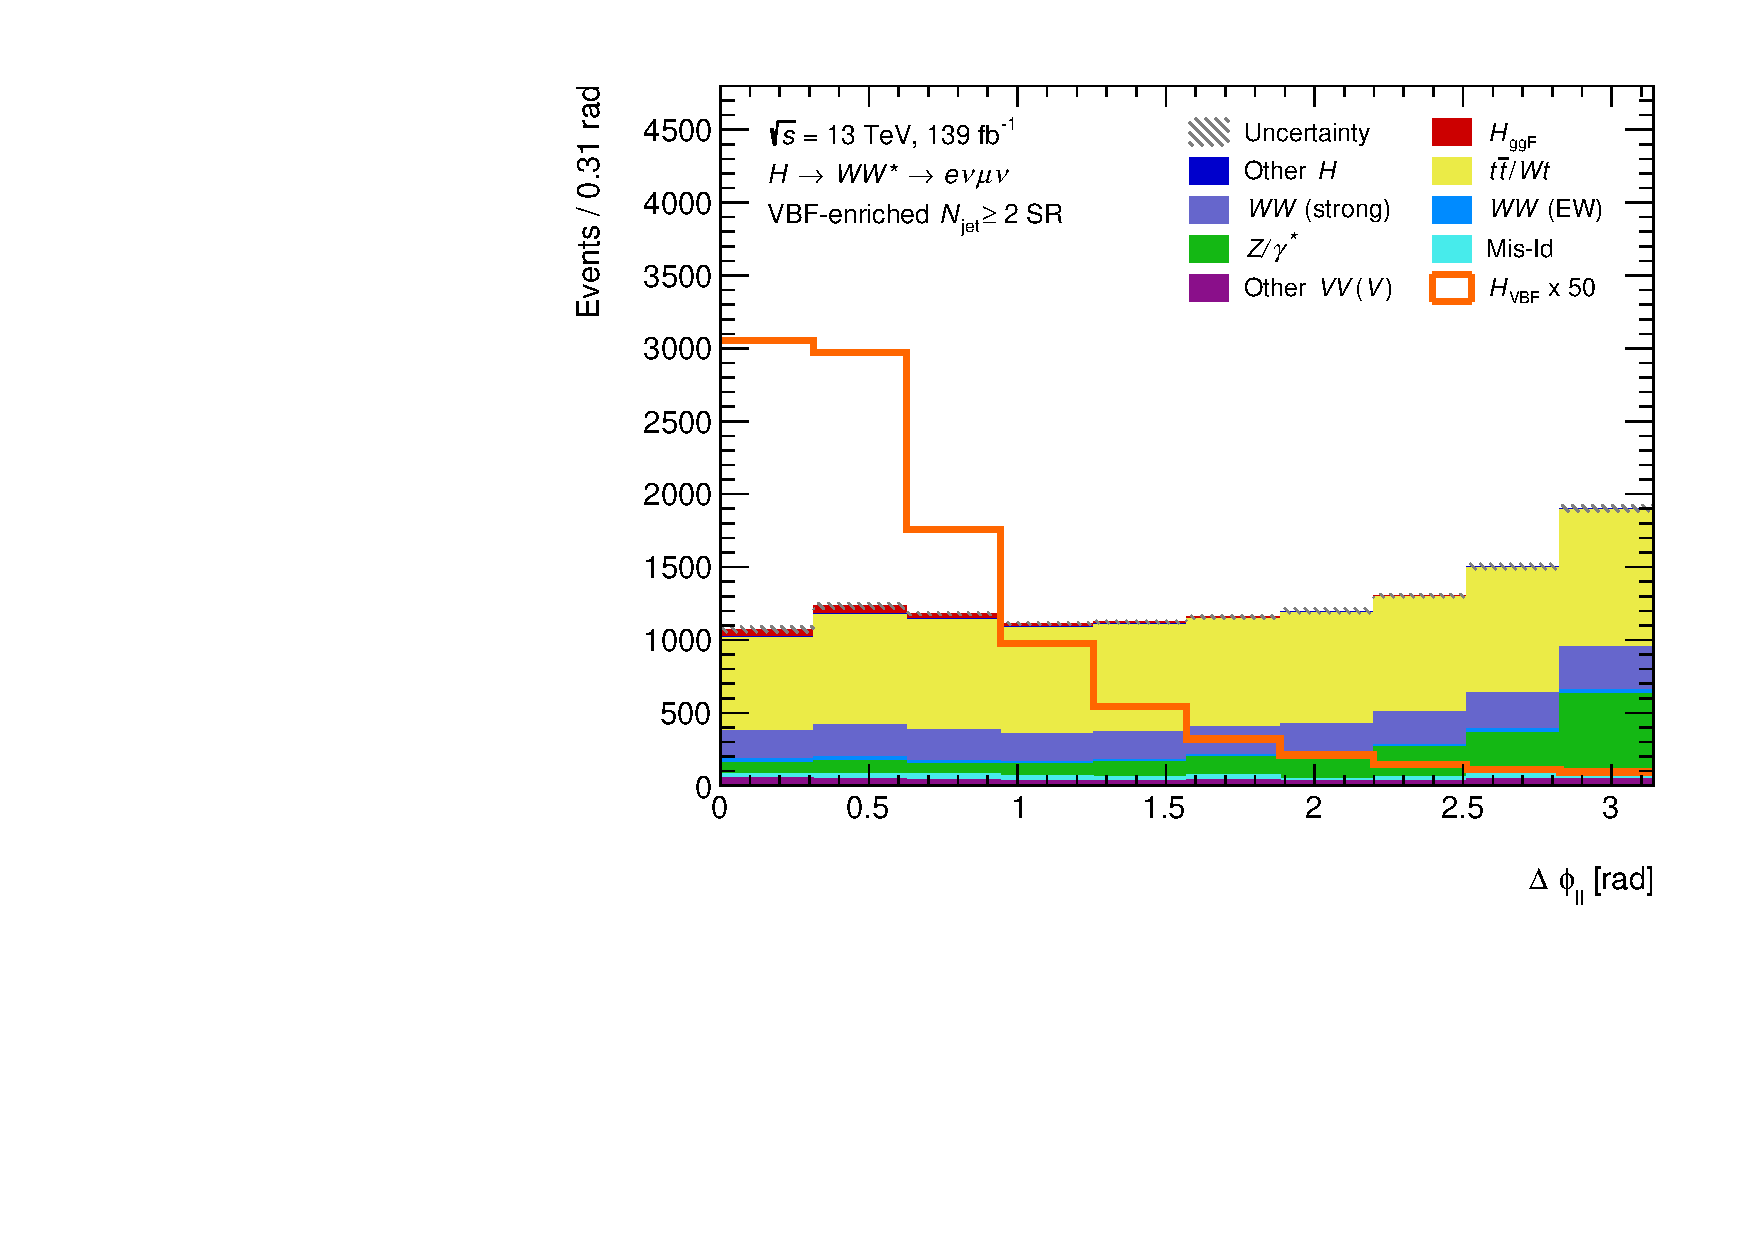
\includegraphics[width=0.32\textwidth]{figures/hww/dnn/blinded/run2-emme-CutVBF_SR-DPhill-lin.pdf} \hfill
        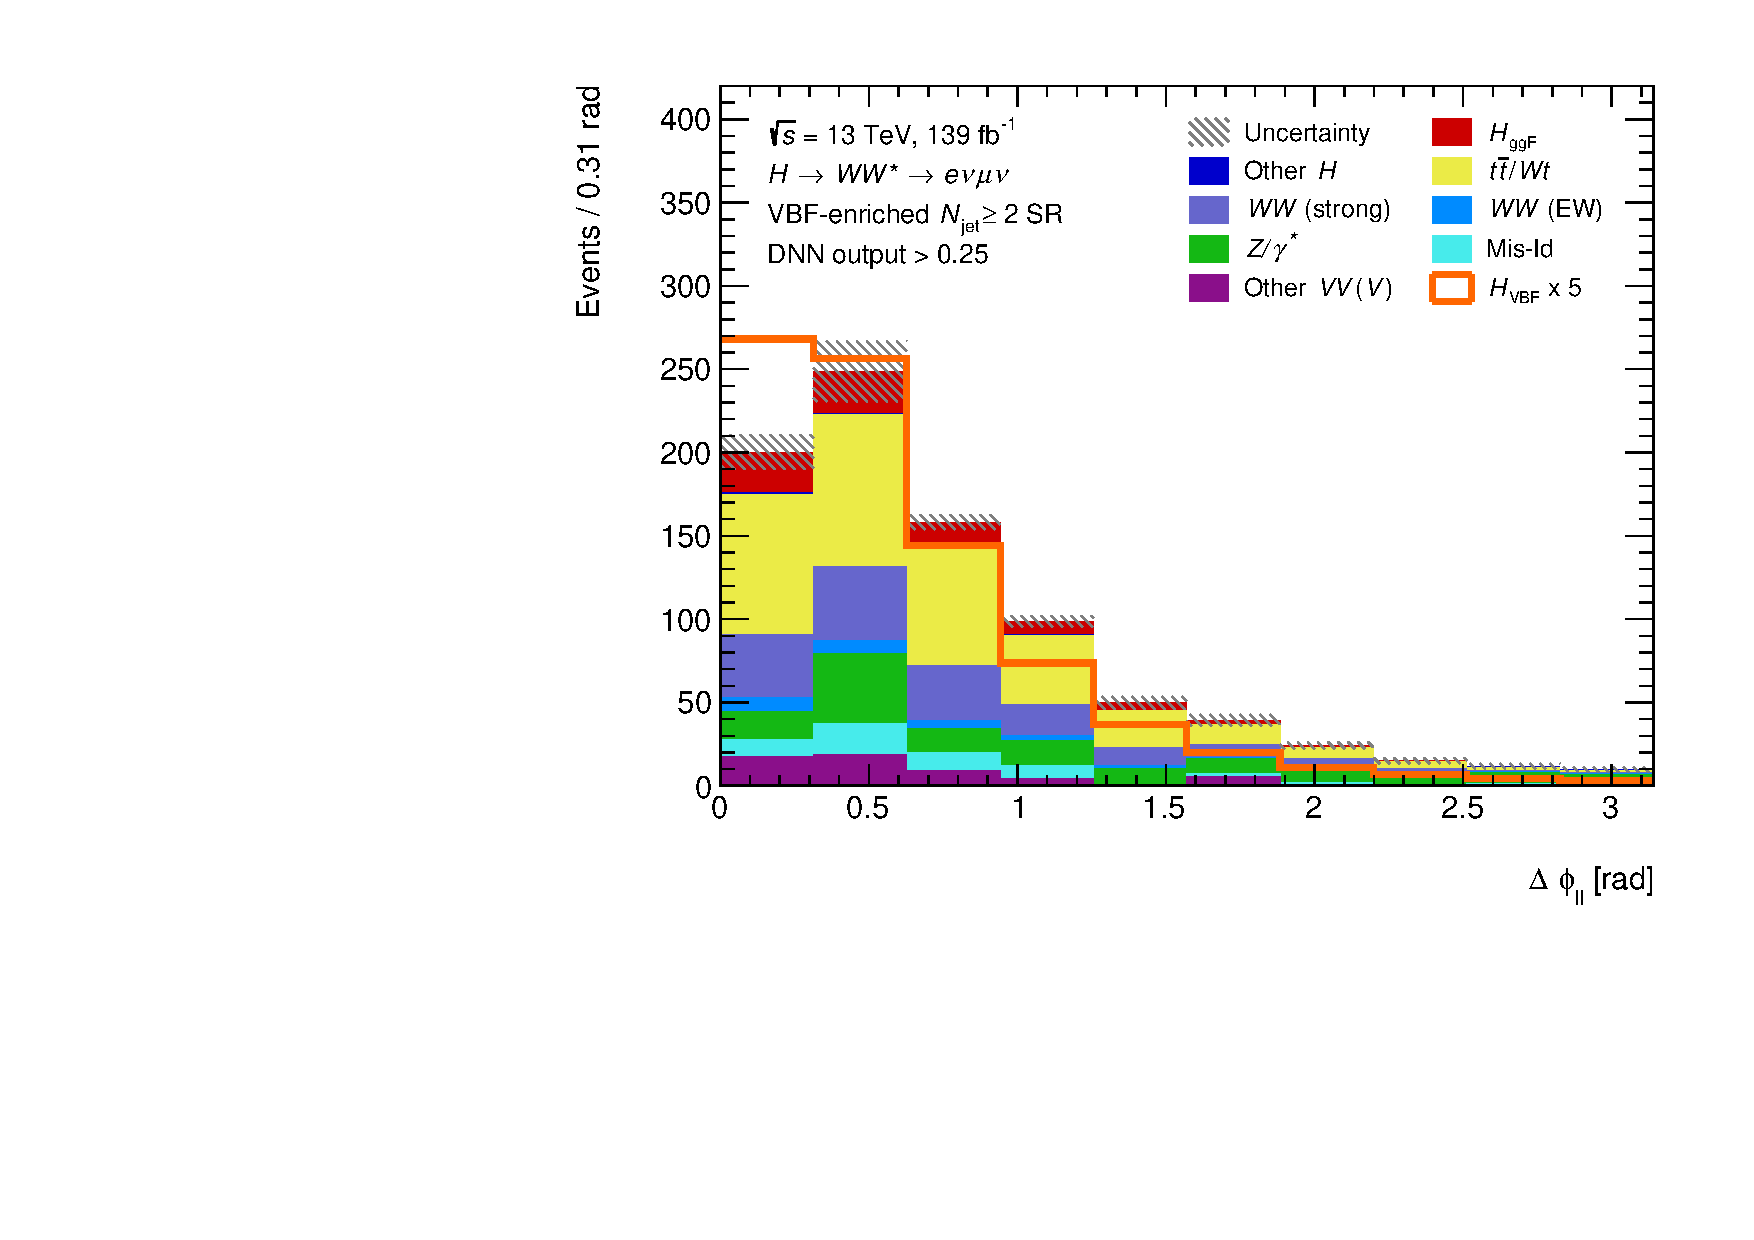
\includegraphics[width=0.32\textwidth]{figures/hww/dnn/blinded/run2-emme-CutVBFSR_DNN25-DPhill-lin.pdf} \hfill
        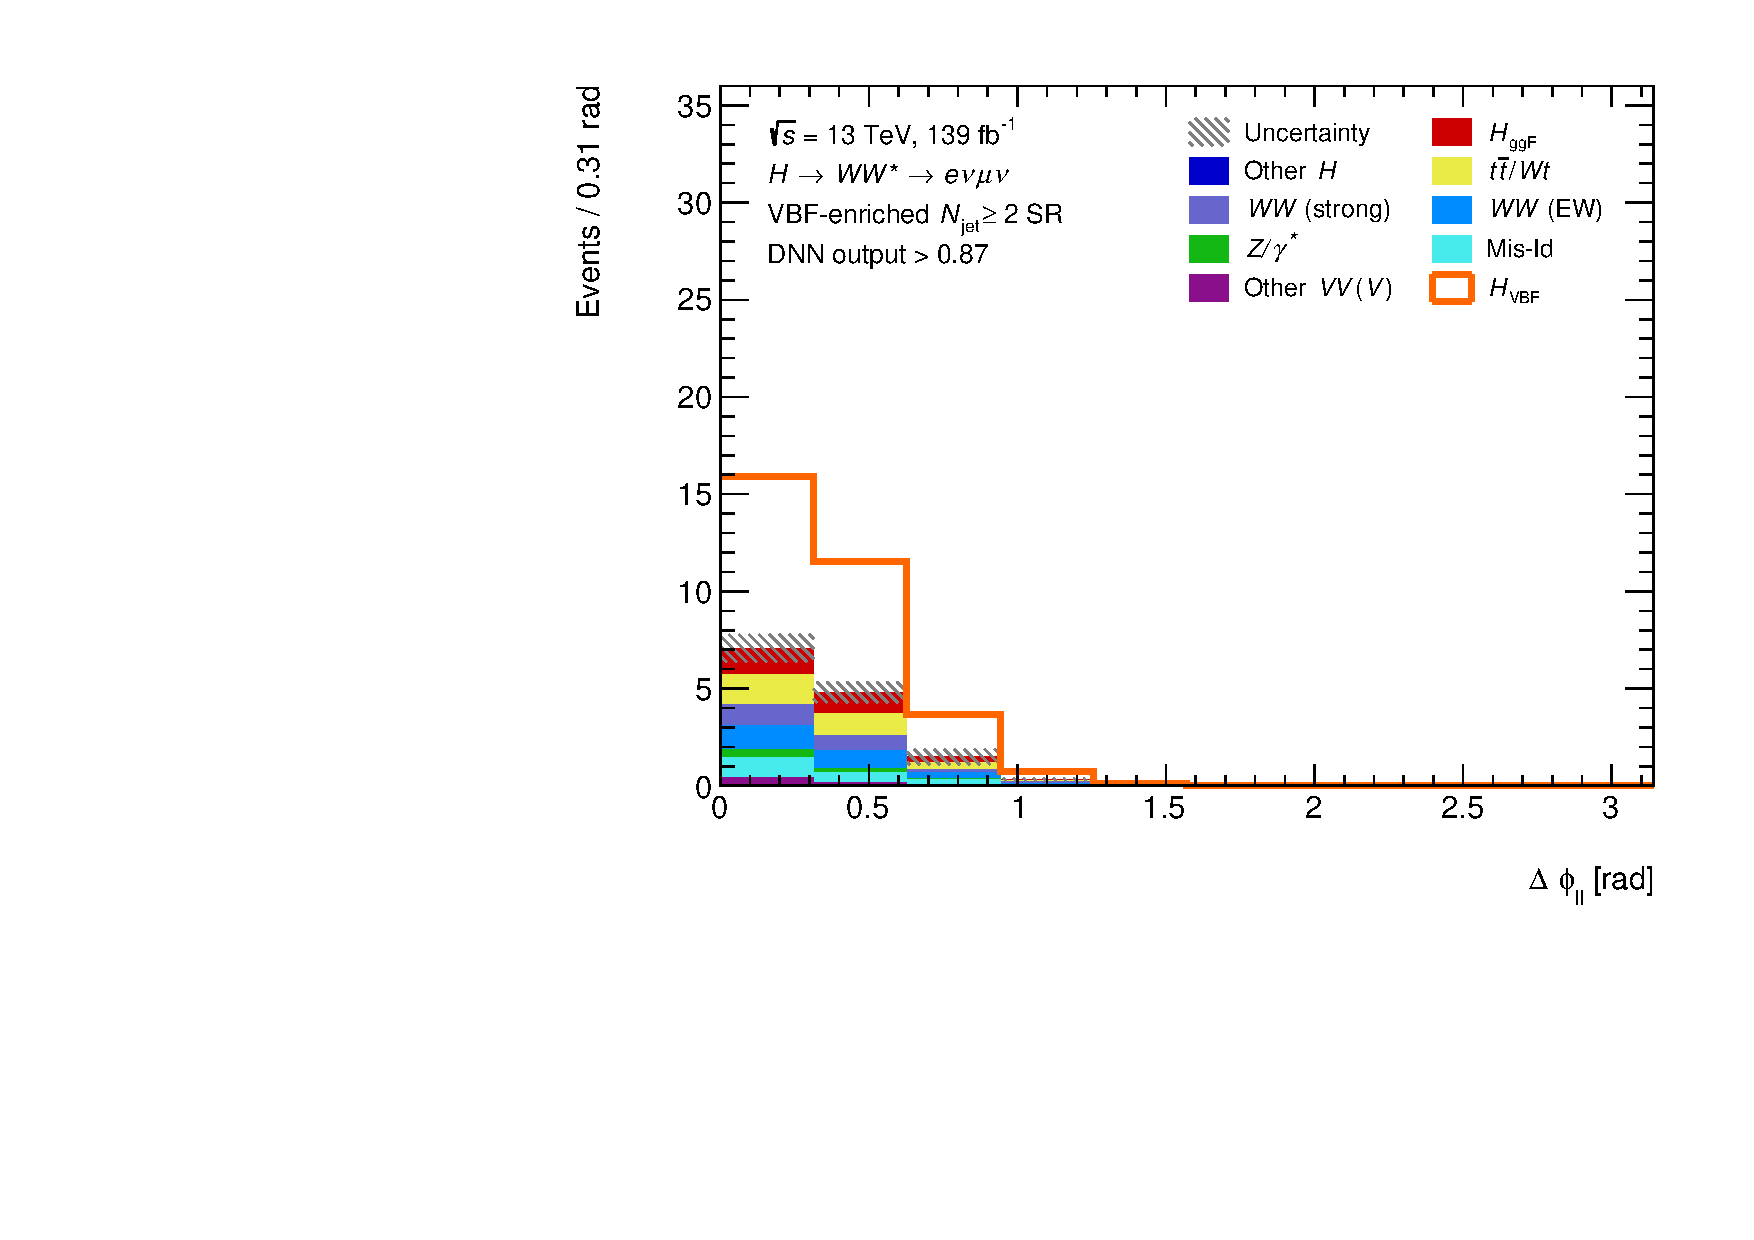
\includegraphics[width=0.32\textwidth]{figures/hww/dnn/blinded/run2-emme-CutVBFSR_DNN87-DPhill-lin.pdf}
    } \\
    \subfloat[$\mll$]{
        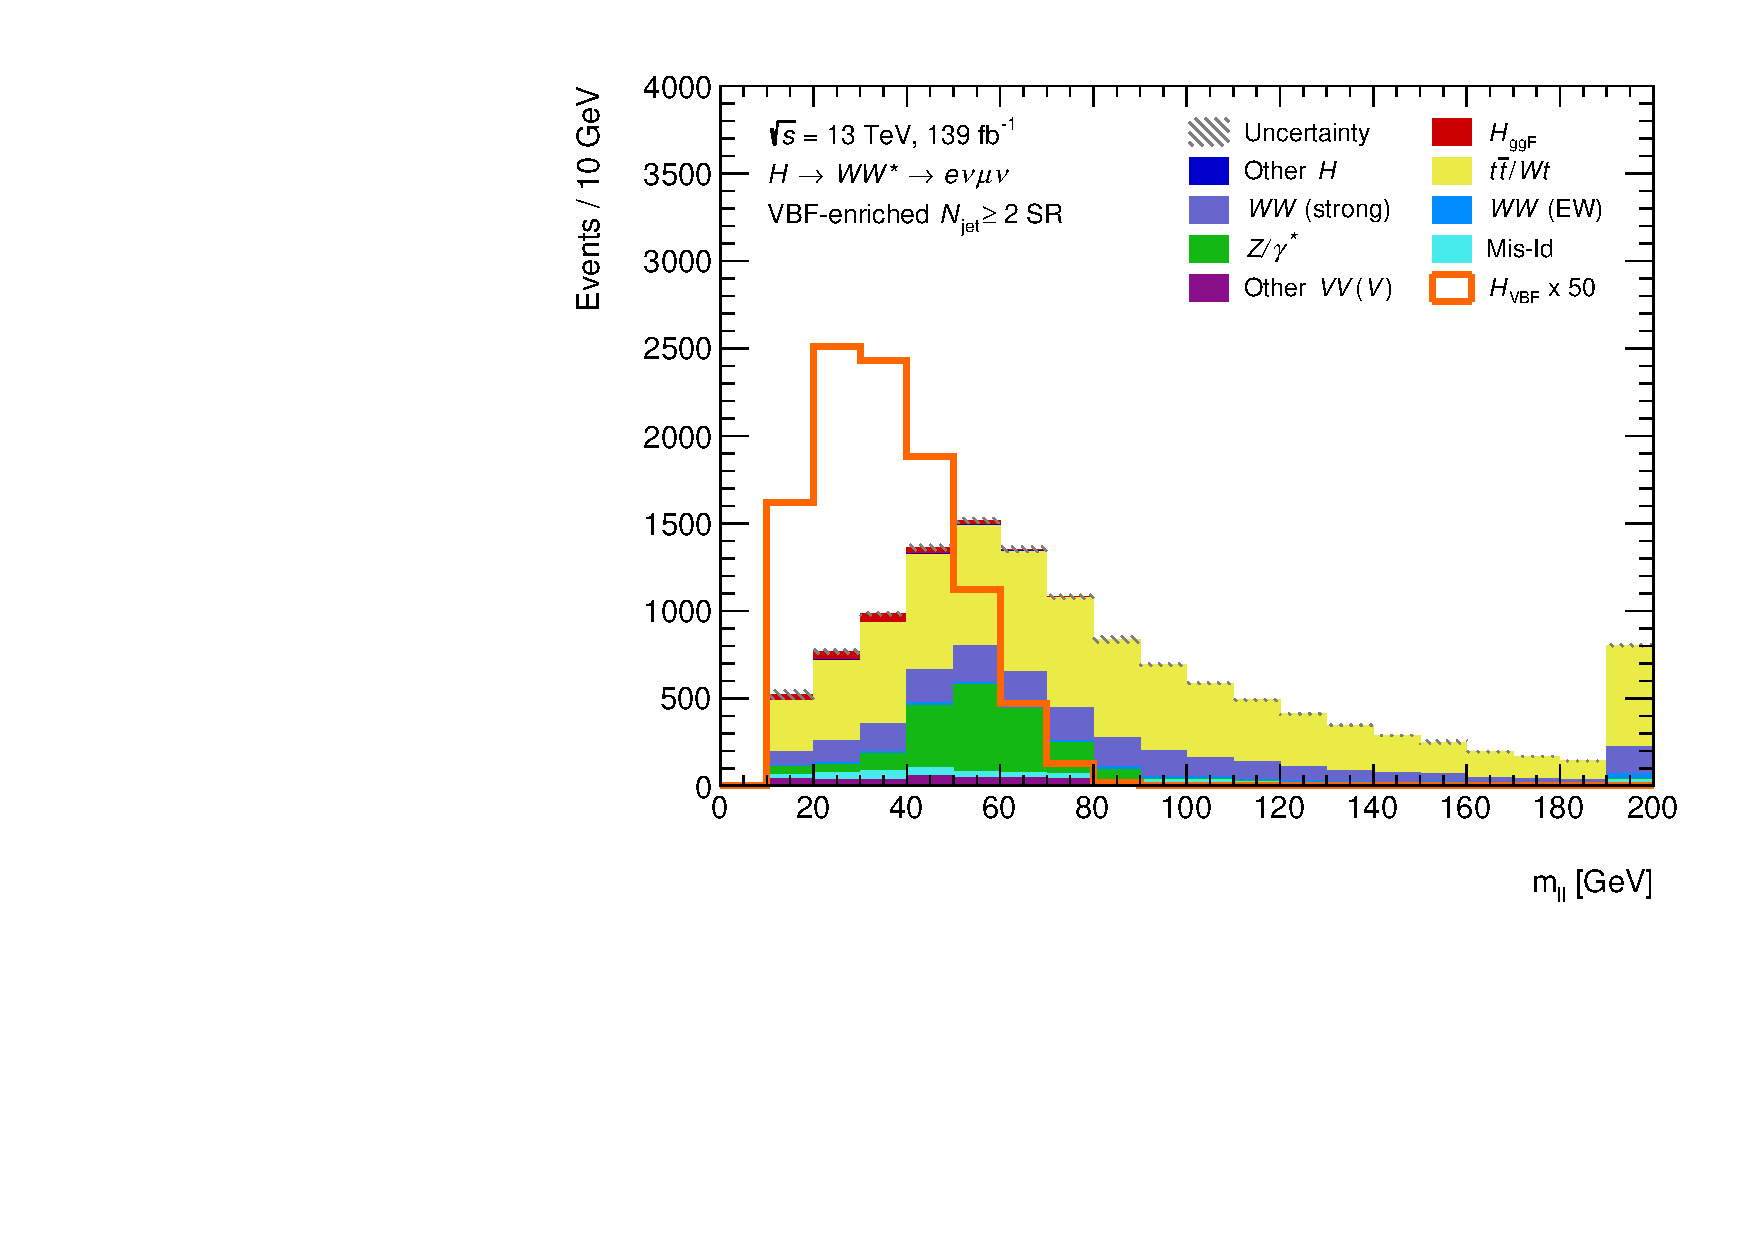
\includegraphics[width=0.32\textwidth]{figures/hww/dnn/blinded/run2-emme-CutVBF_SR-Mll-lin.pdf}
        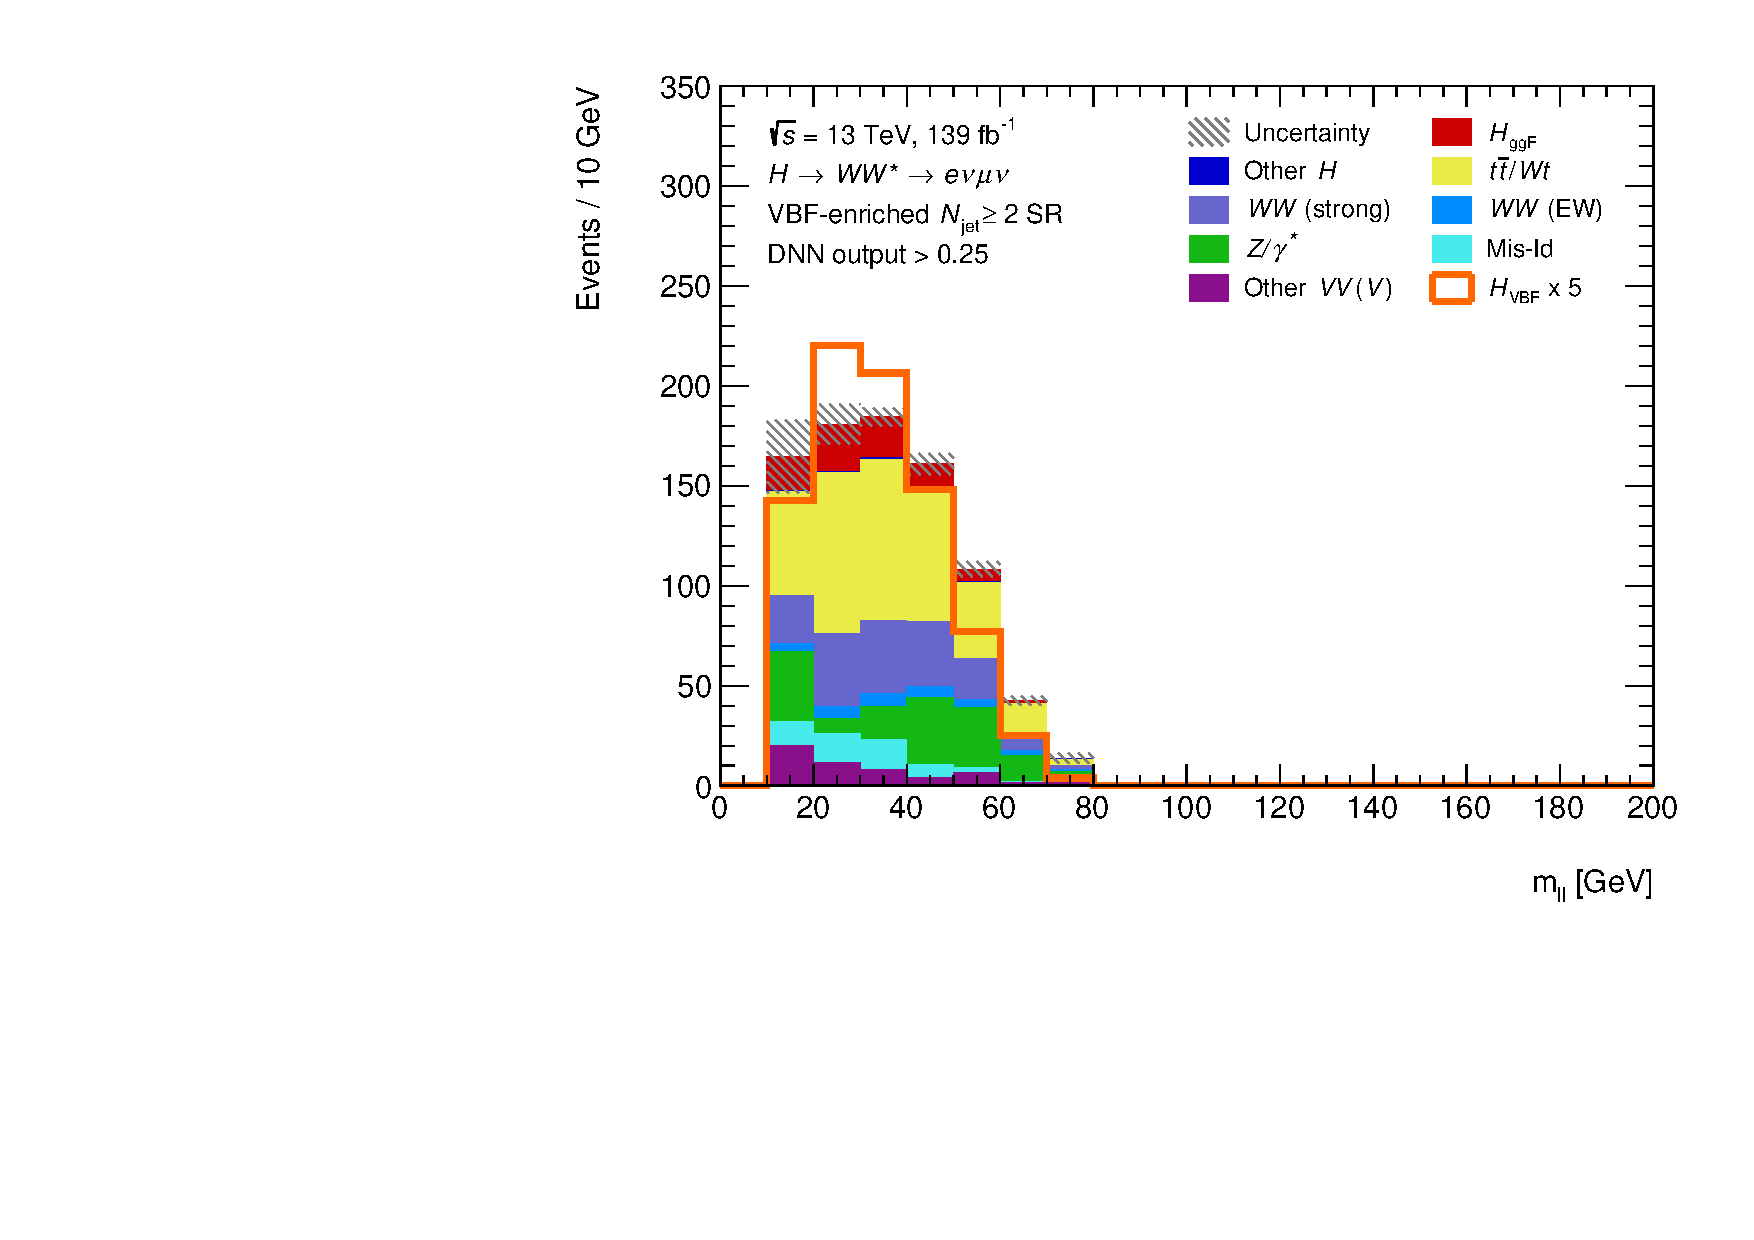
\includegraphics[width=0.32\textwidth]{figures/hww/dnn/blinded/run2-emme-CutVBFSR_DNN25-Mll-lin.pdf}
        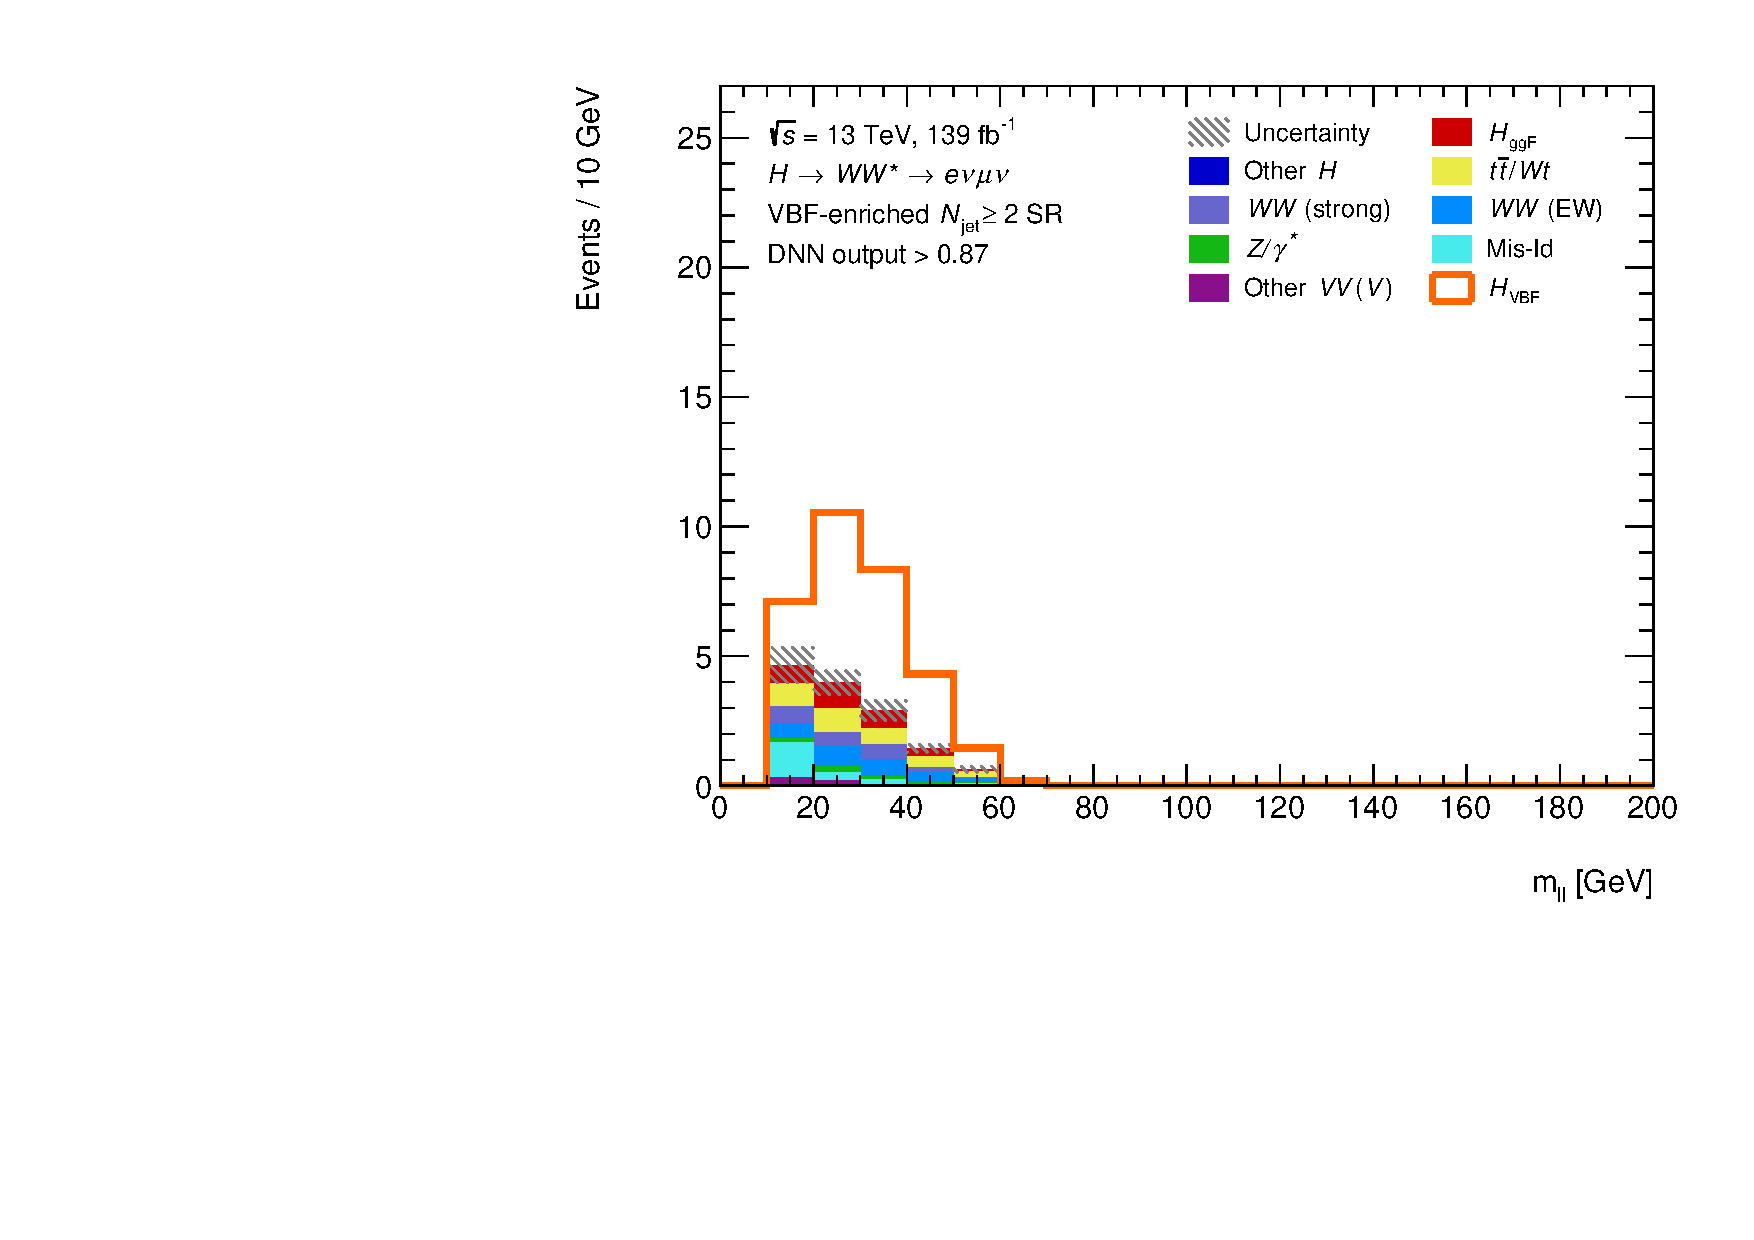
\includegraphics[width=0.32\textwidth]{figures/hww/dnn/blinded/run2-emme-CutVBFSR_DNN87-Mll-lin.pdf}
    } \\
    \subfloat[$\dyjj$]{
        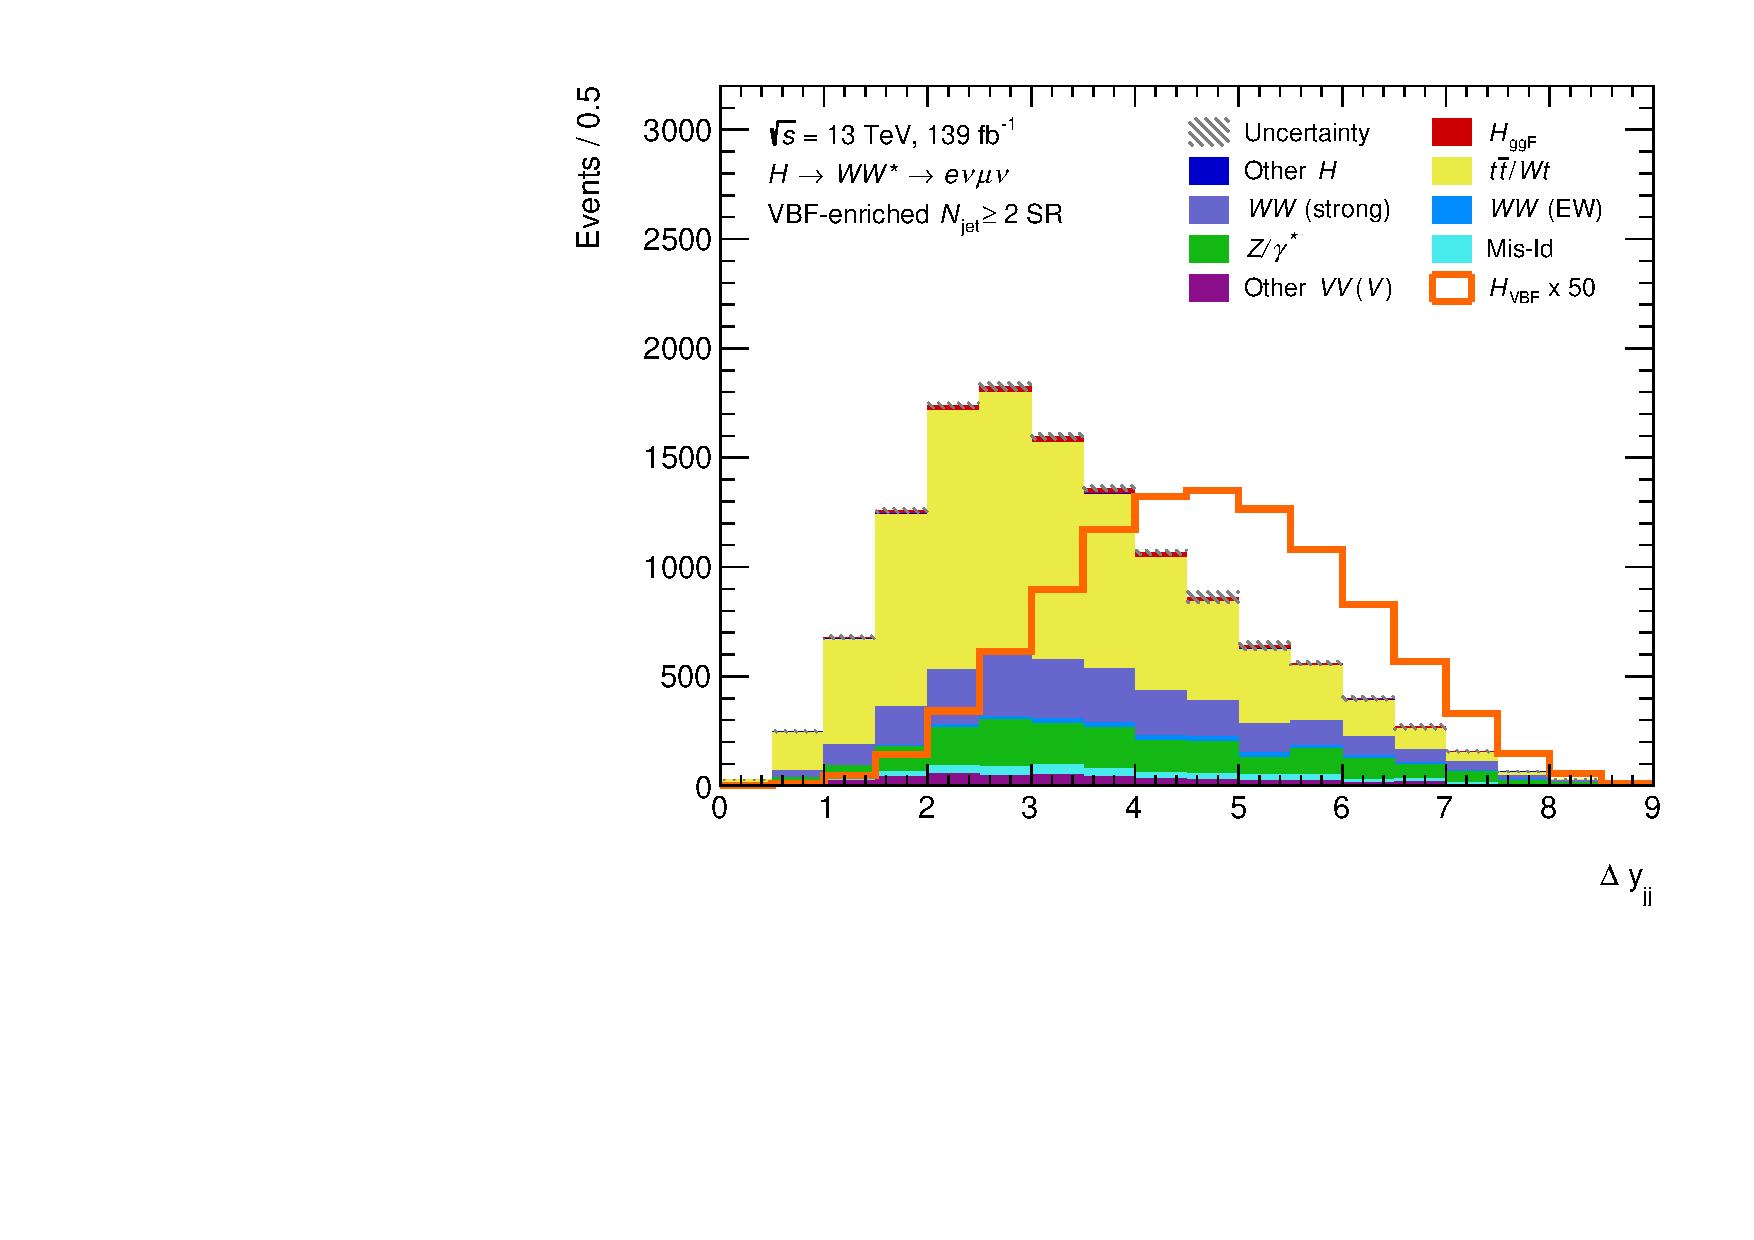
\includegraphics[width=0.32\textwidth]{figures/hww/dnn/blinded/run2-emme-CutVBF_SR-DYjj-lin.pdf} \hfill
        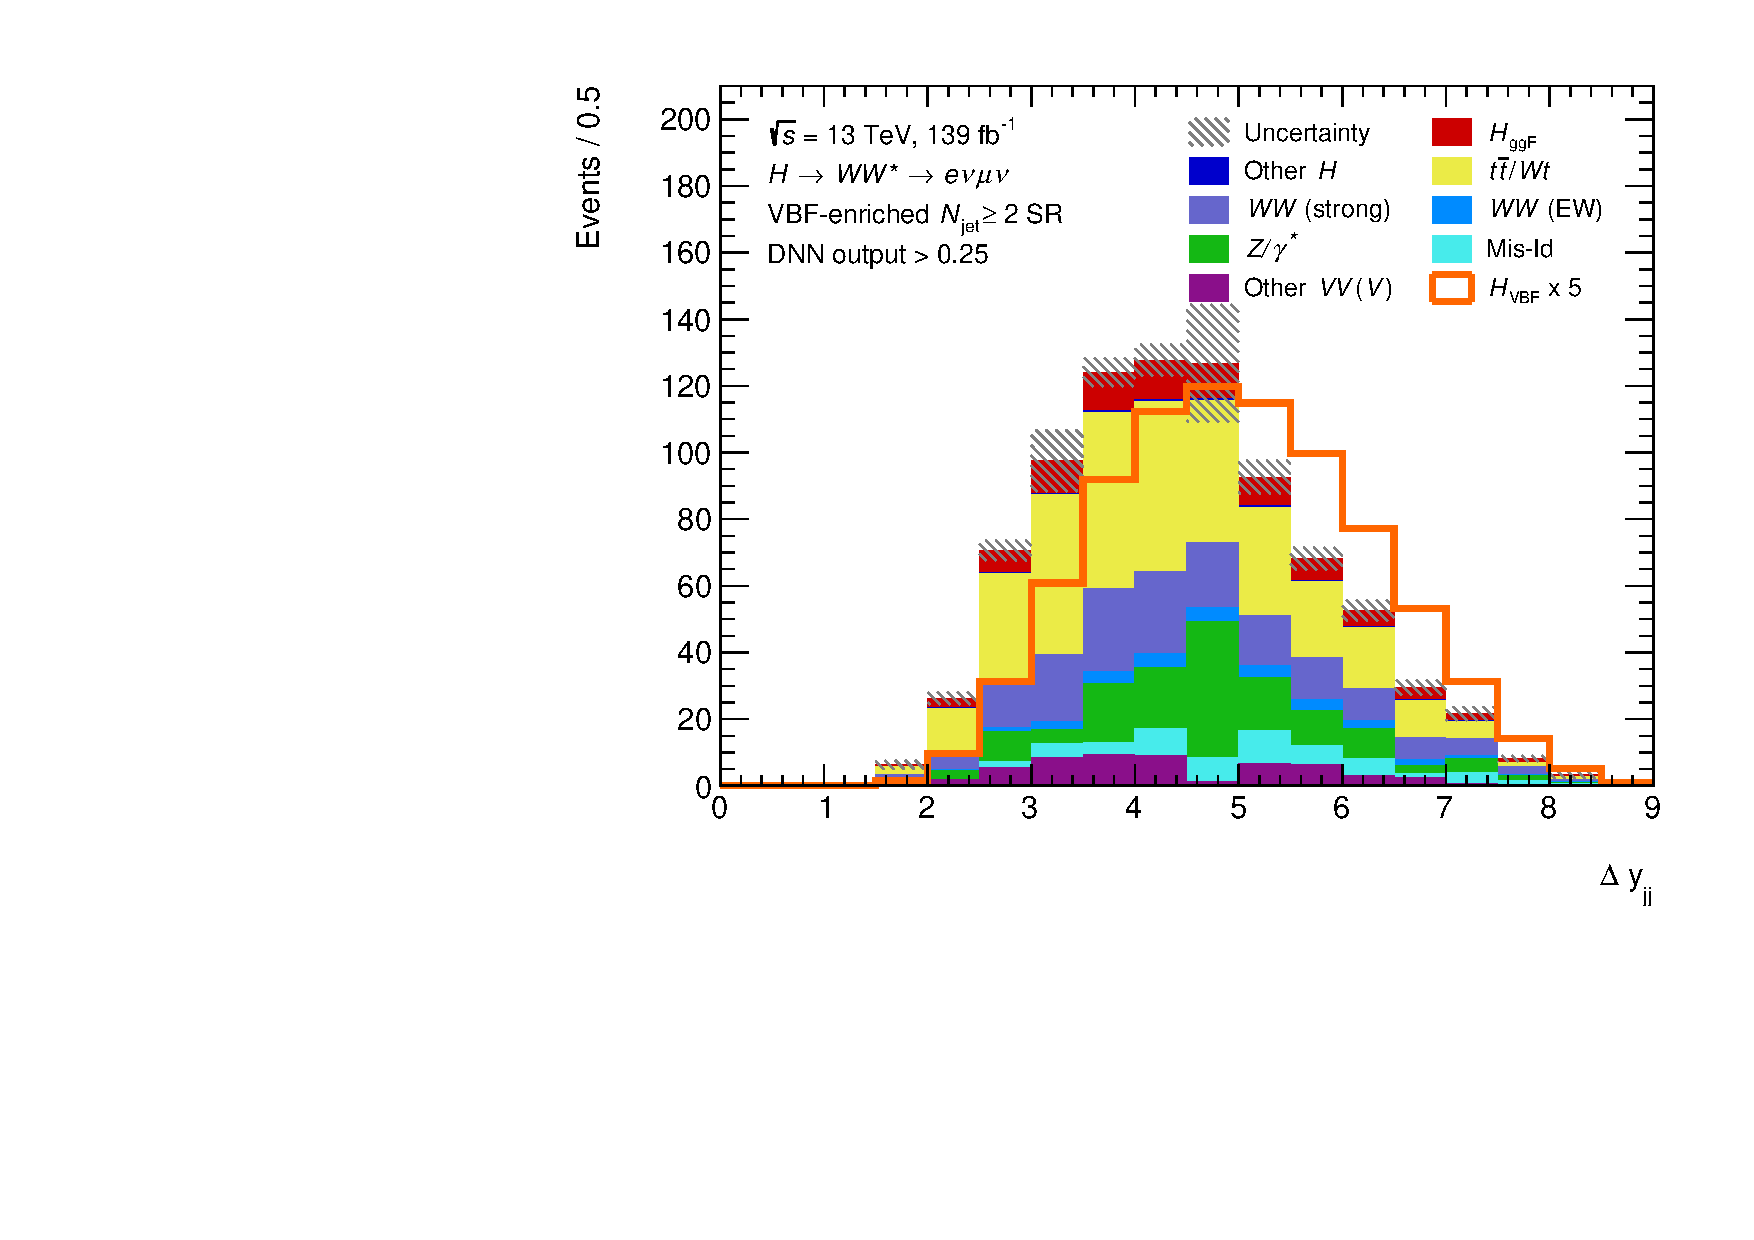
\includegraphics[width=0.32\textwidth]{figures/hww/dnn/blinded/run2-emme-CutVBFSR_DNN25-DYjj-lin.pdf} \hfill
        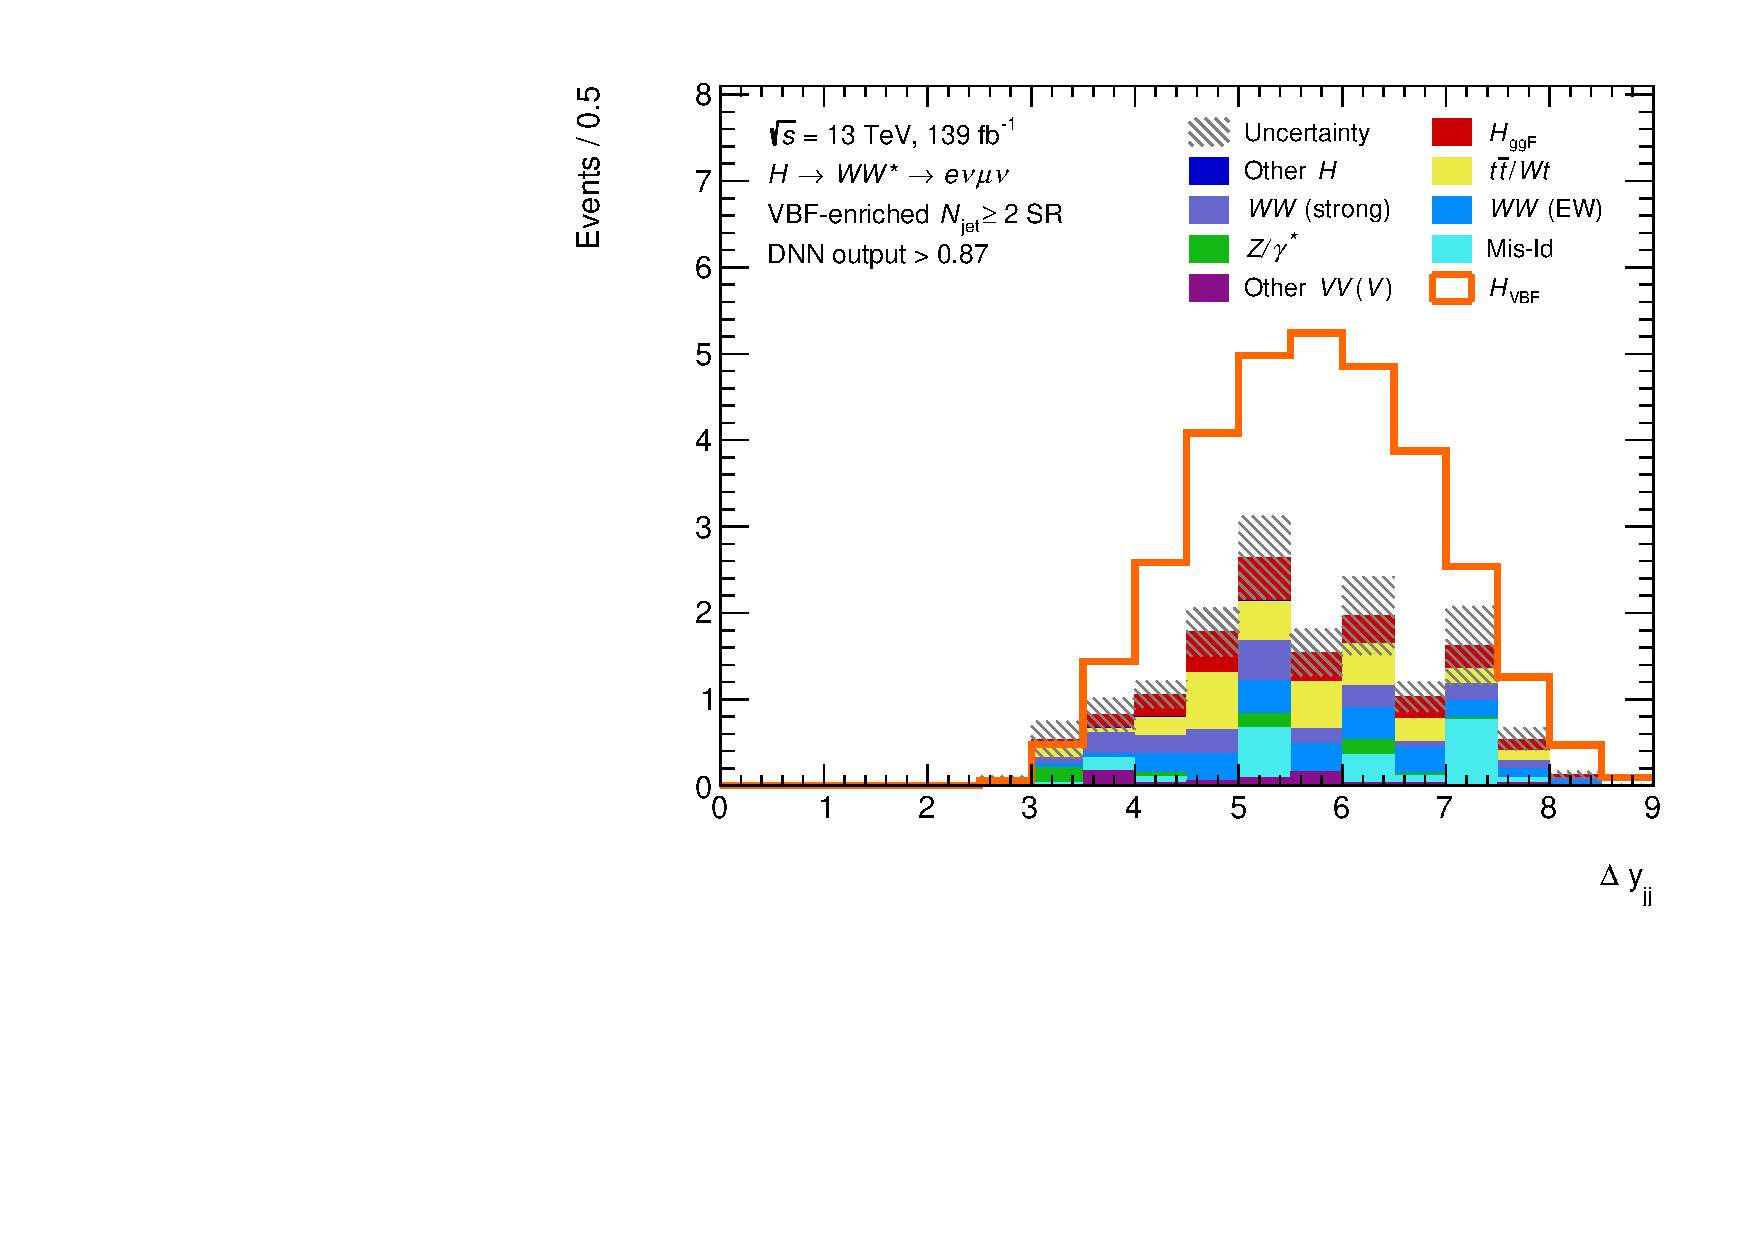
\includegraphics[width=0.32\textwidth]{figures/hww/dnn/blinded/run2-emme-CutVBFSR_DNN87-DYjj-lin.pdf}
    } \\
    \subfloat[$\mjj$]{
        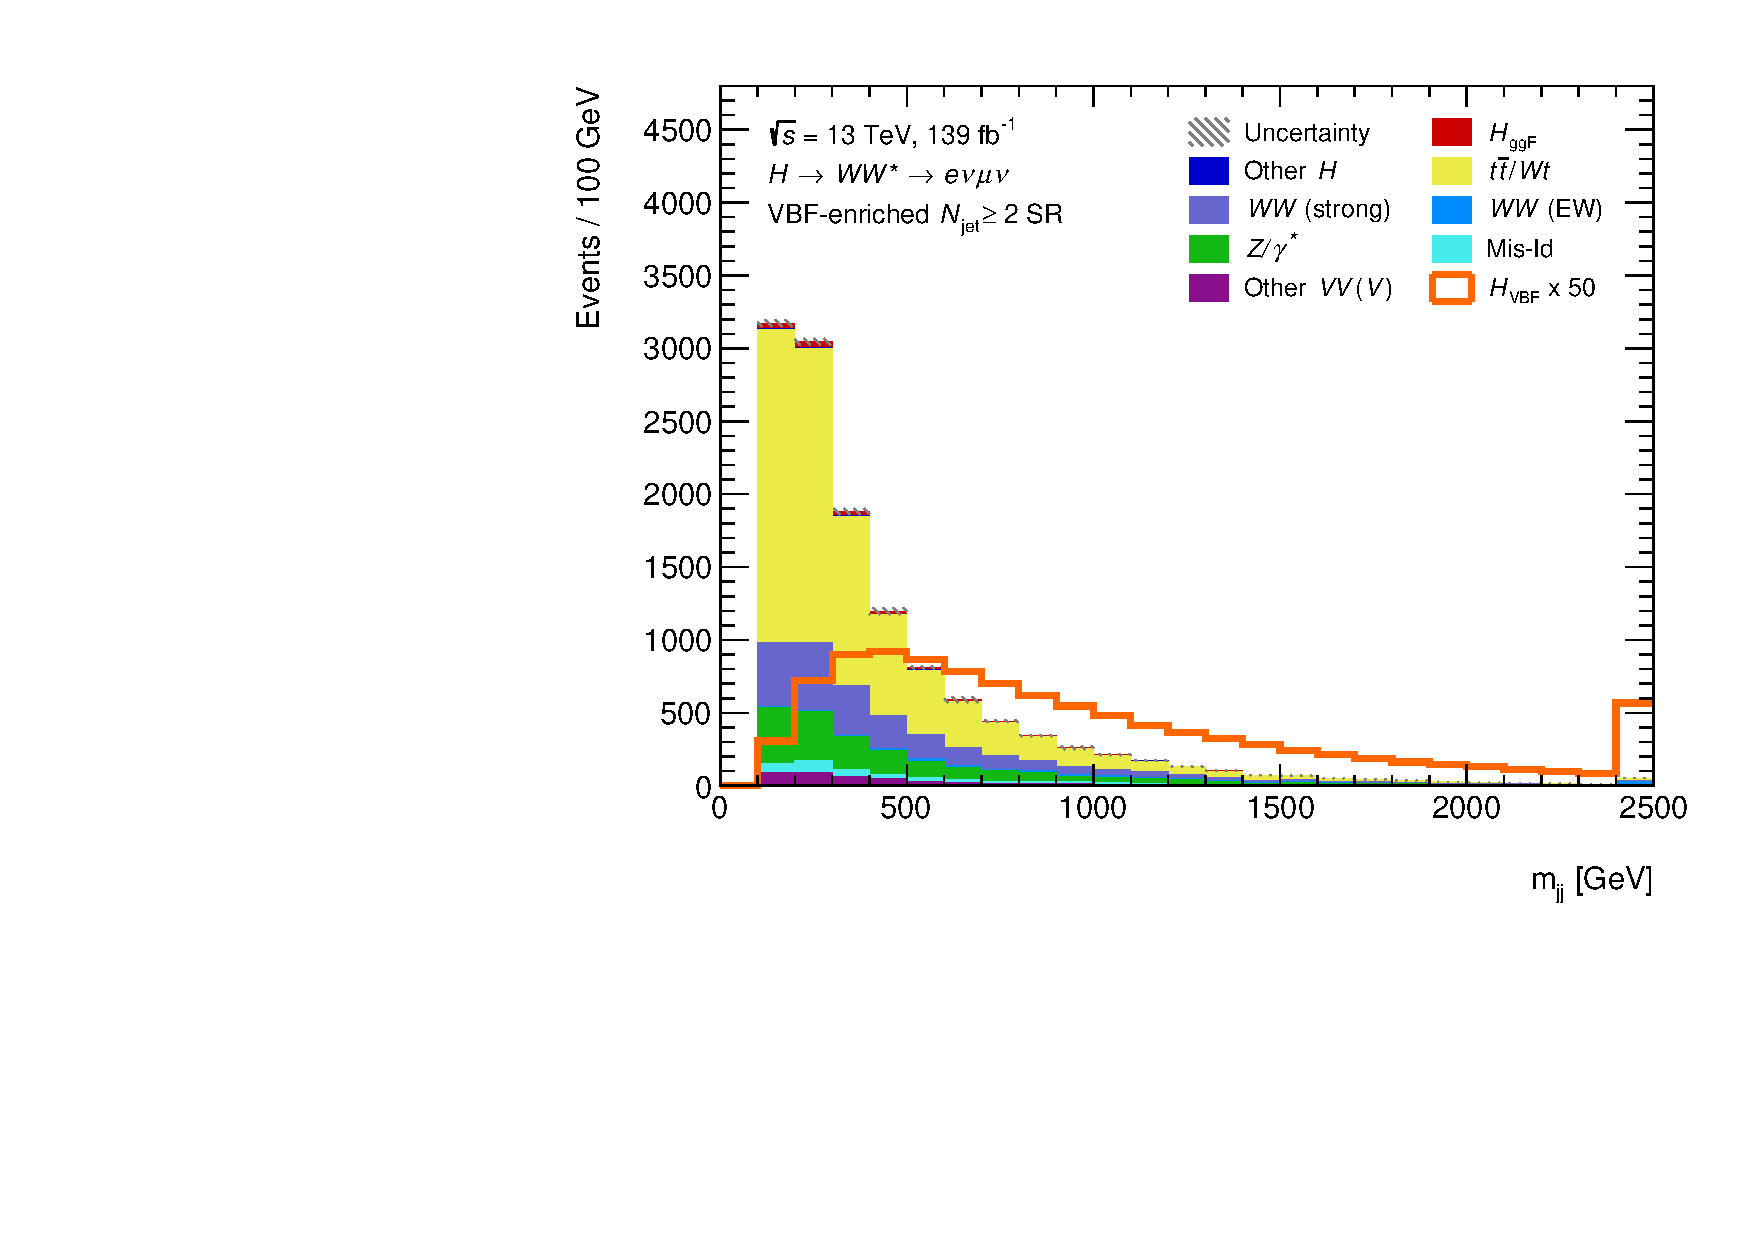
\includegraphics[width=0.32\textwidth]{figures/hww/dnn/blinded/run2-emme-CutVBF_SR-Mjj-lin.pdf} \hfill
        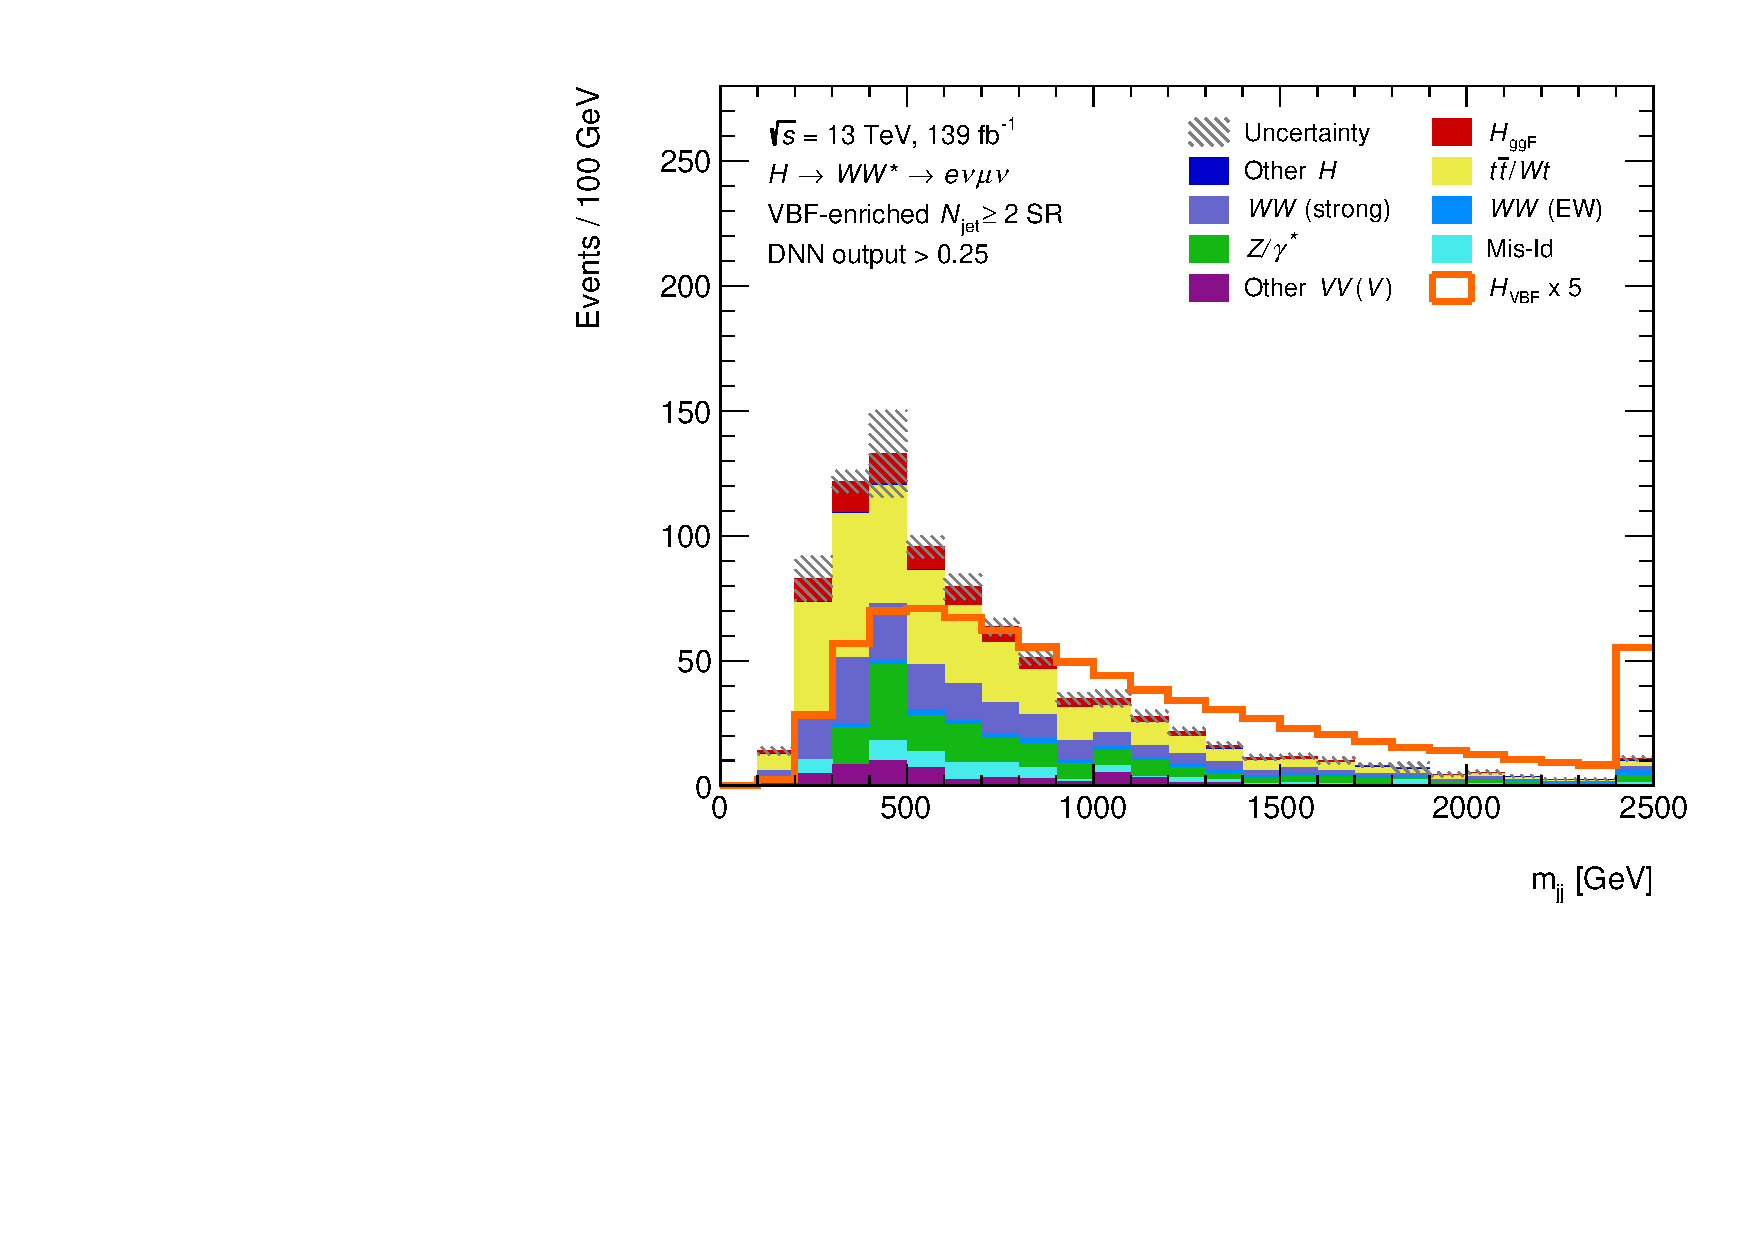
\includegraphics[width=0.32\textwidth]{figures/hww/dnn/blinded/run2-emme-CutVBFSR_DNN25-Mjj-lin.pdf} \hfill
        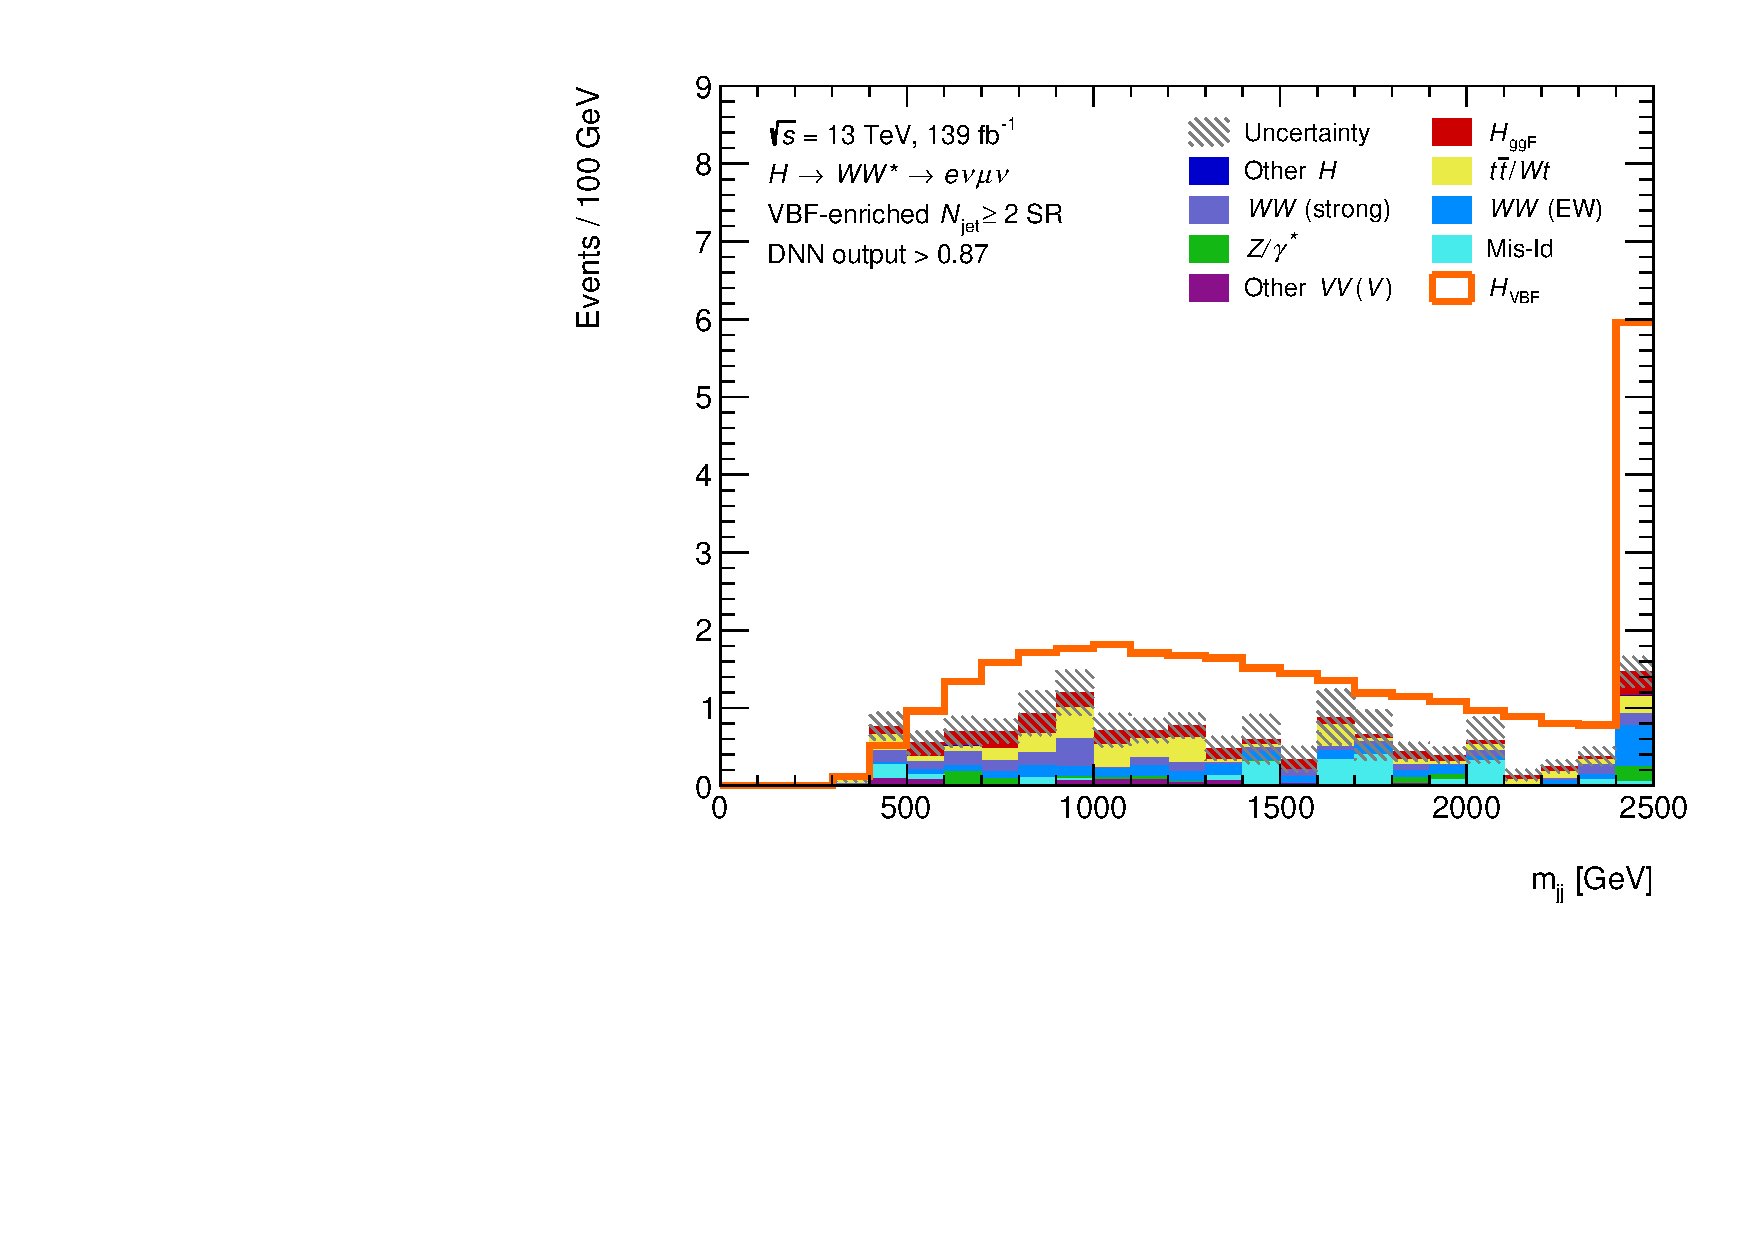
\includegraphics[width=0.32\textwidth]{figures/hww/dnn/blinded/run2-emme-CutVBFSR_DNN87-Mjj-lin.pdf}
    } \\
    {\caption{Distributions of $\dphill$, $\mll$, $\dyjj$, $\mjj$ in the VBF signal region.
        Each row corresponds to one variable with different selections made on the DNN output.
        \label{fig:vbf:blindedSR0} }}
\end{figure}



\begin{figure}[h]
    \centering
    \subfloat[$\mT$]{
        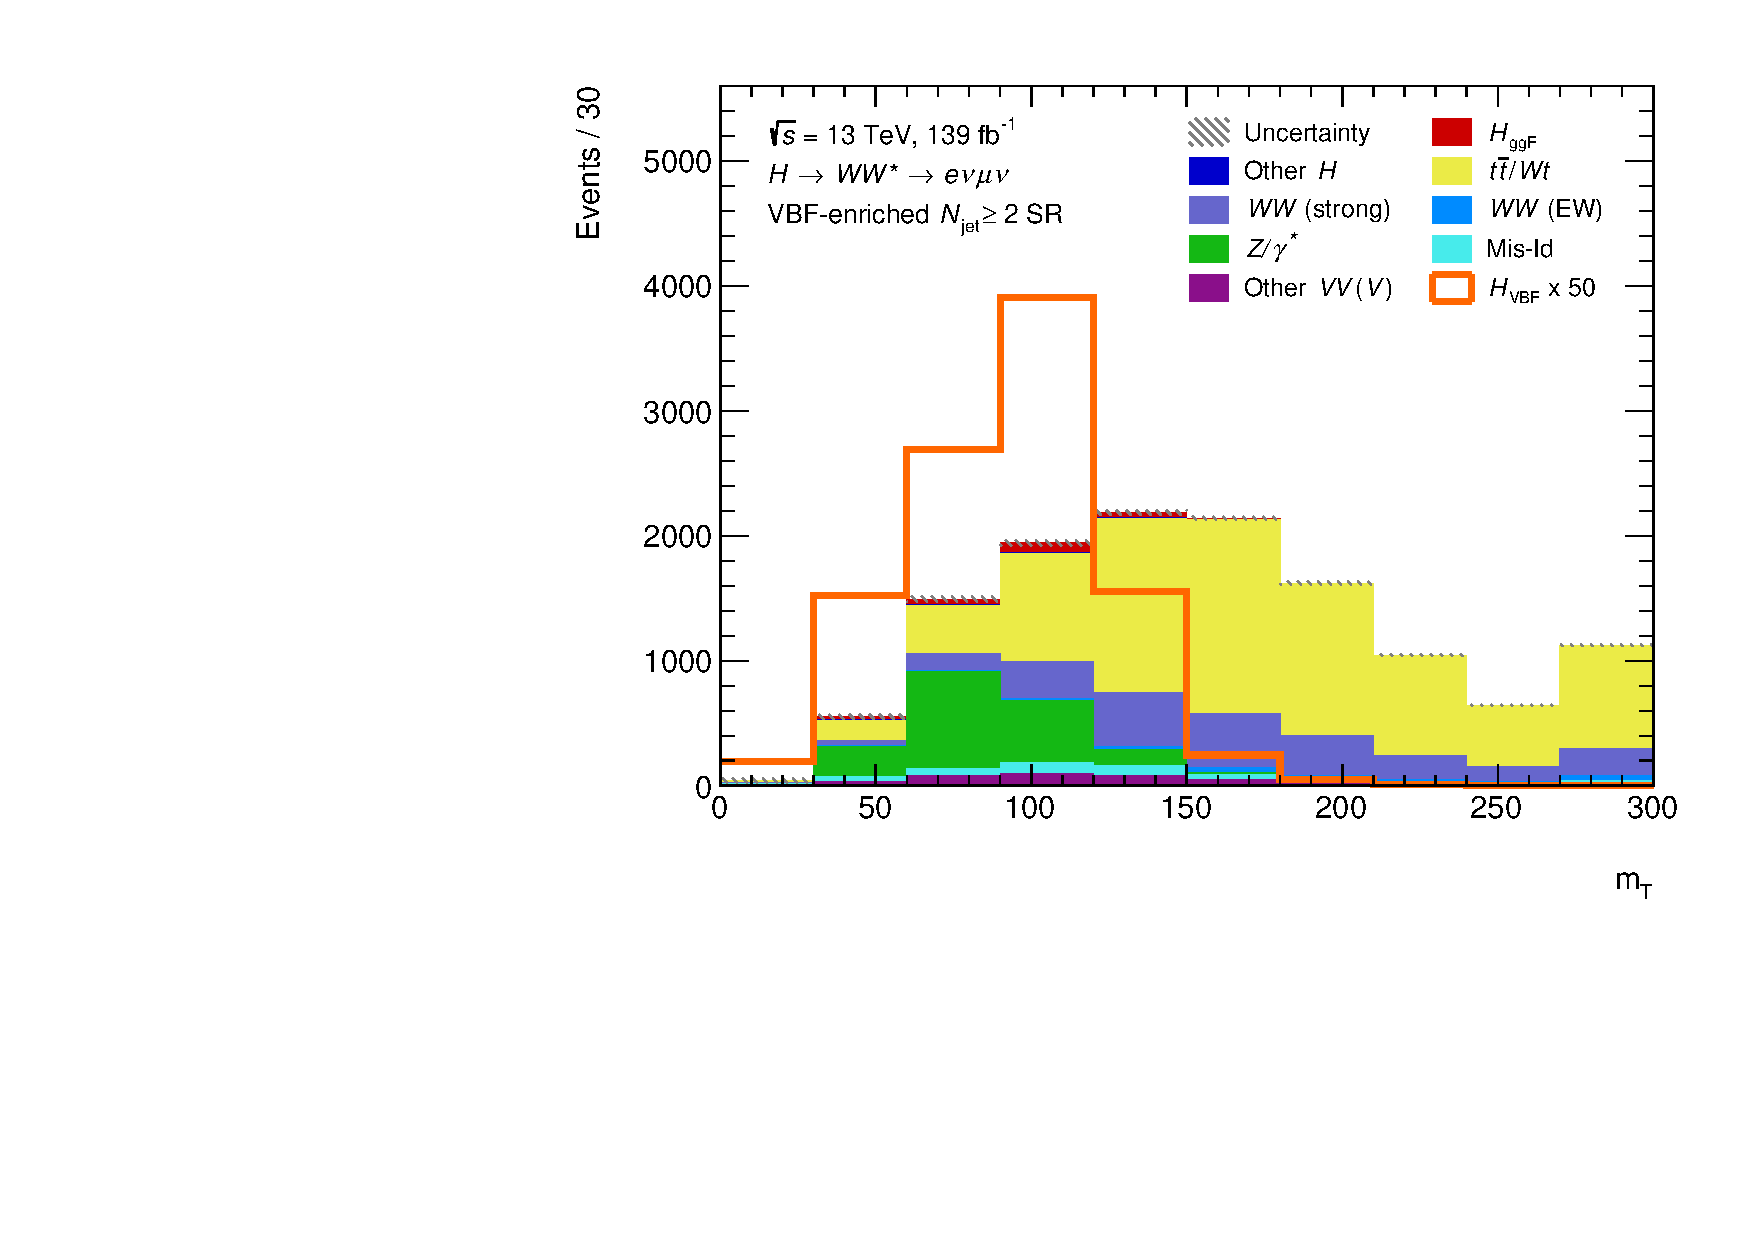
\includegraphics[width=0.32\textwidth]{figures/hww/dnn/blinded/run2-emme-CutVBF_SR-MT-lin.pdf} \hfill
        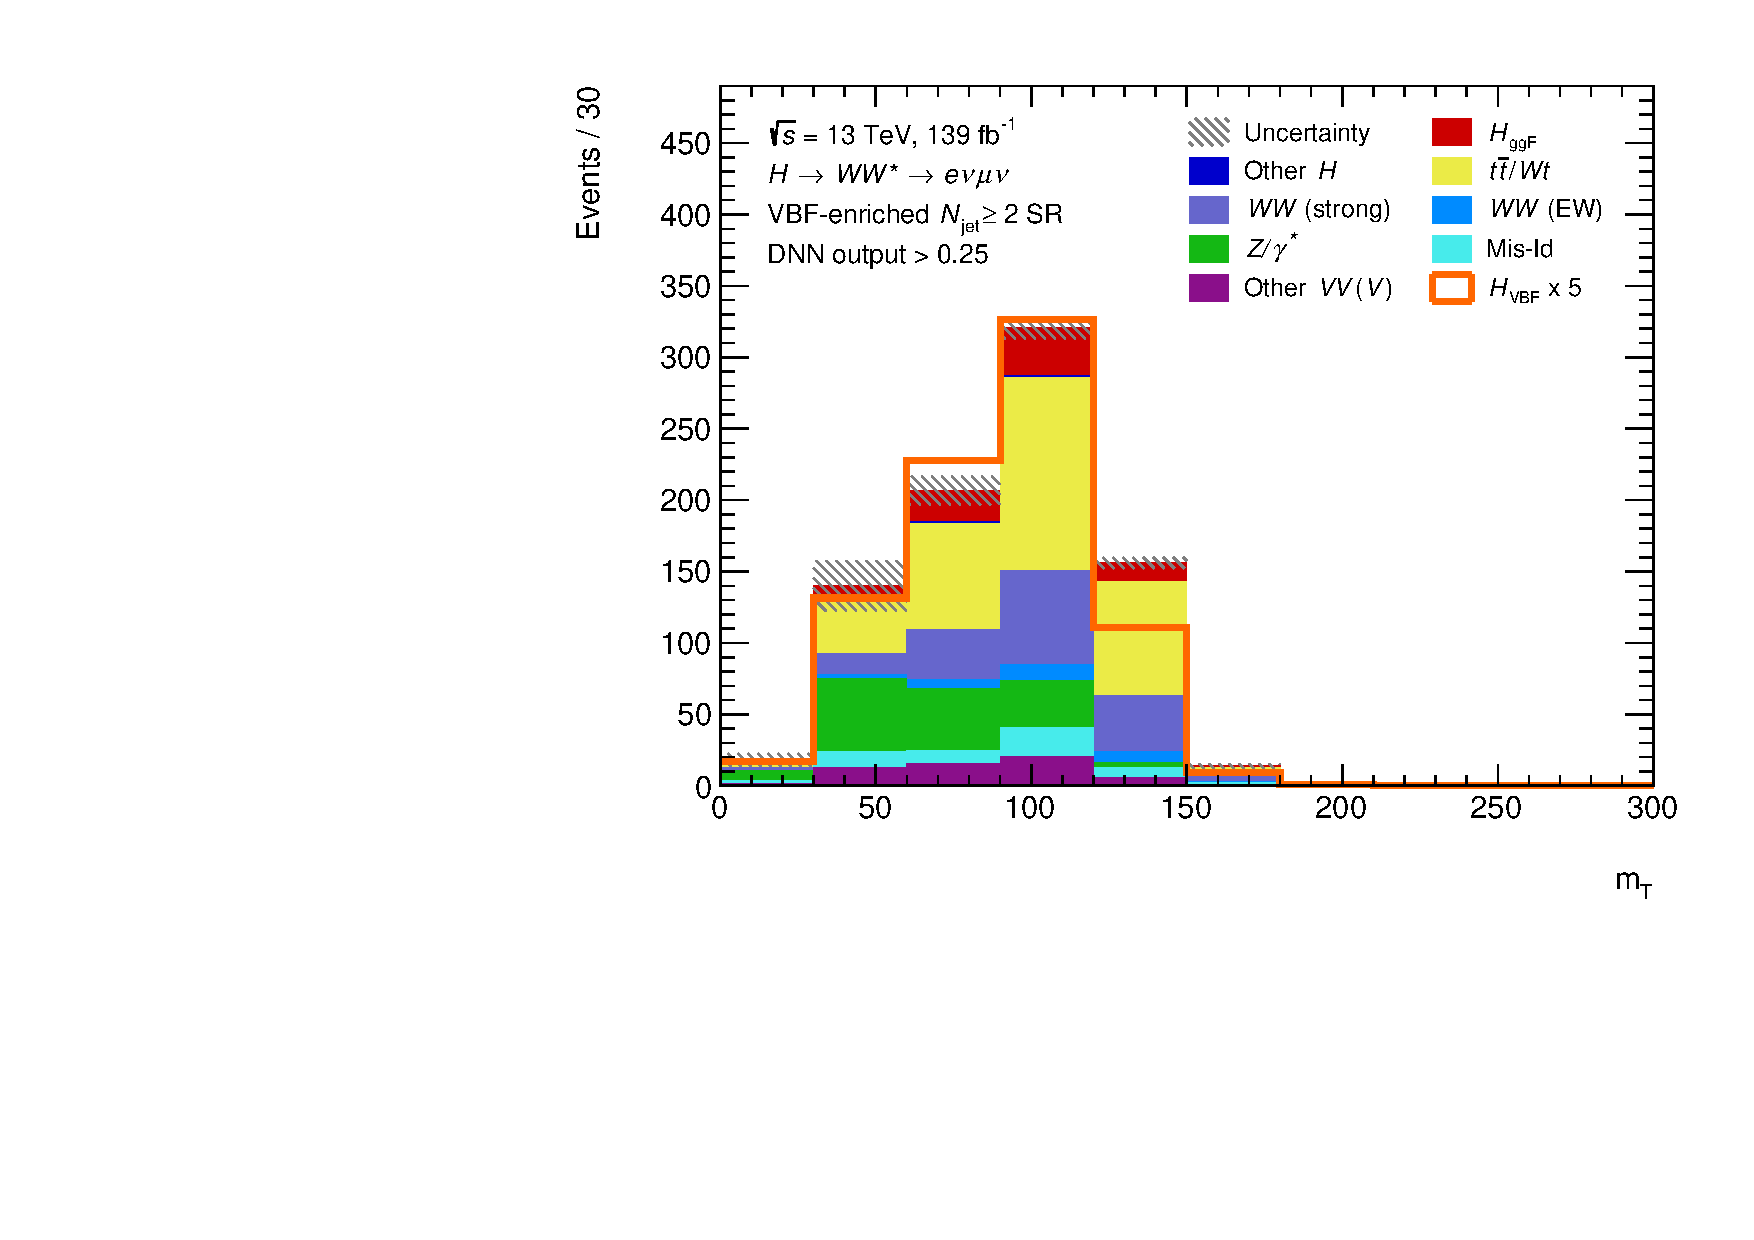
\includegraphics[width=0.32\textwidth]{figures/hww/dnn/blinded/run2-emme-CutVBFSR_DNN25-MT-lin.pdf} \hfill
        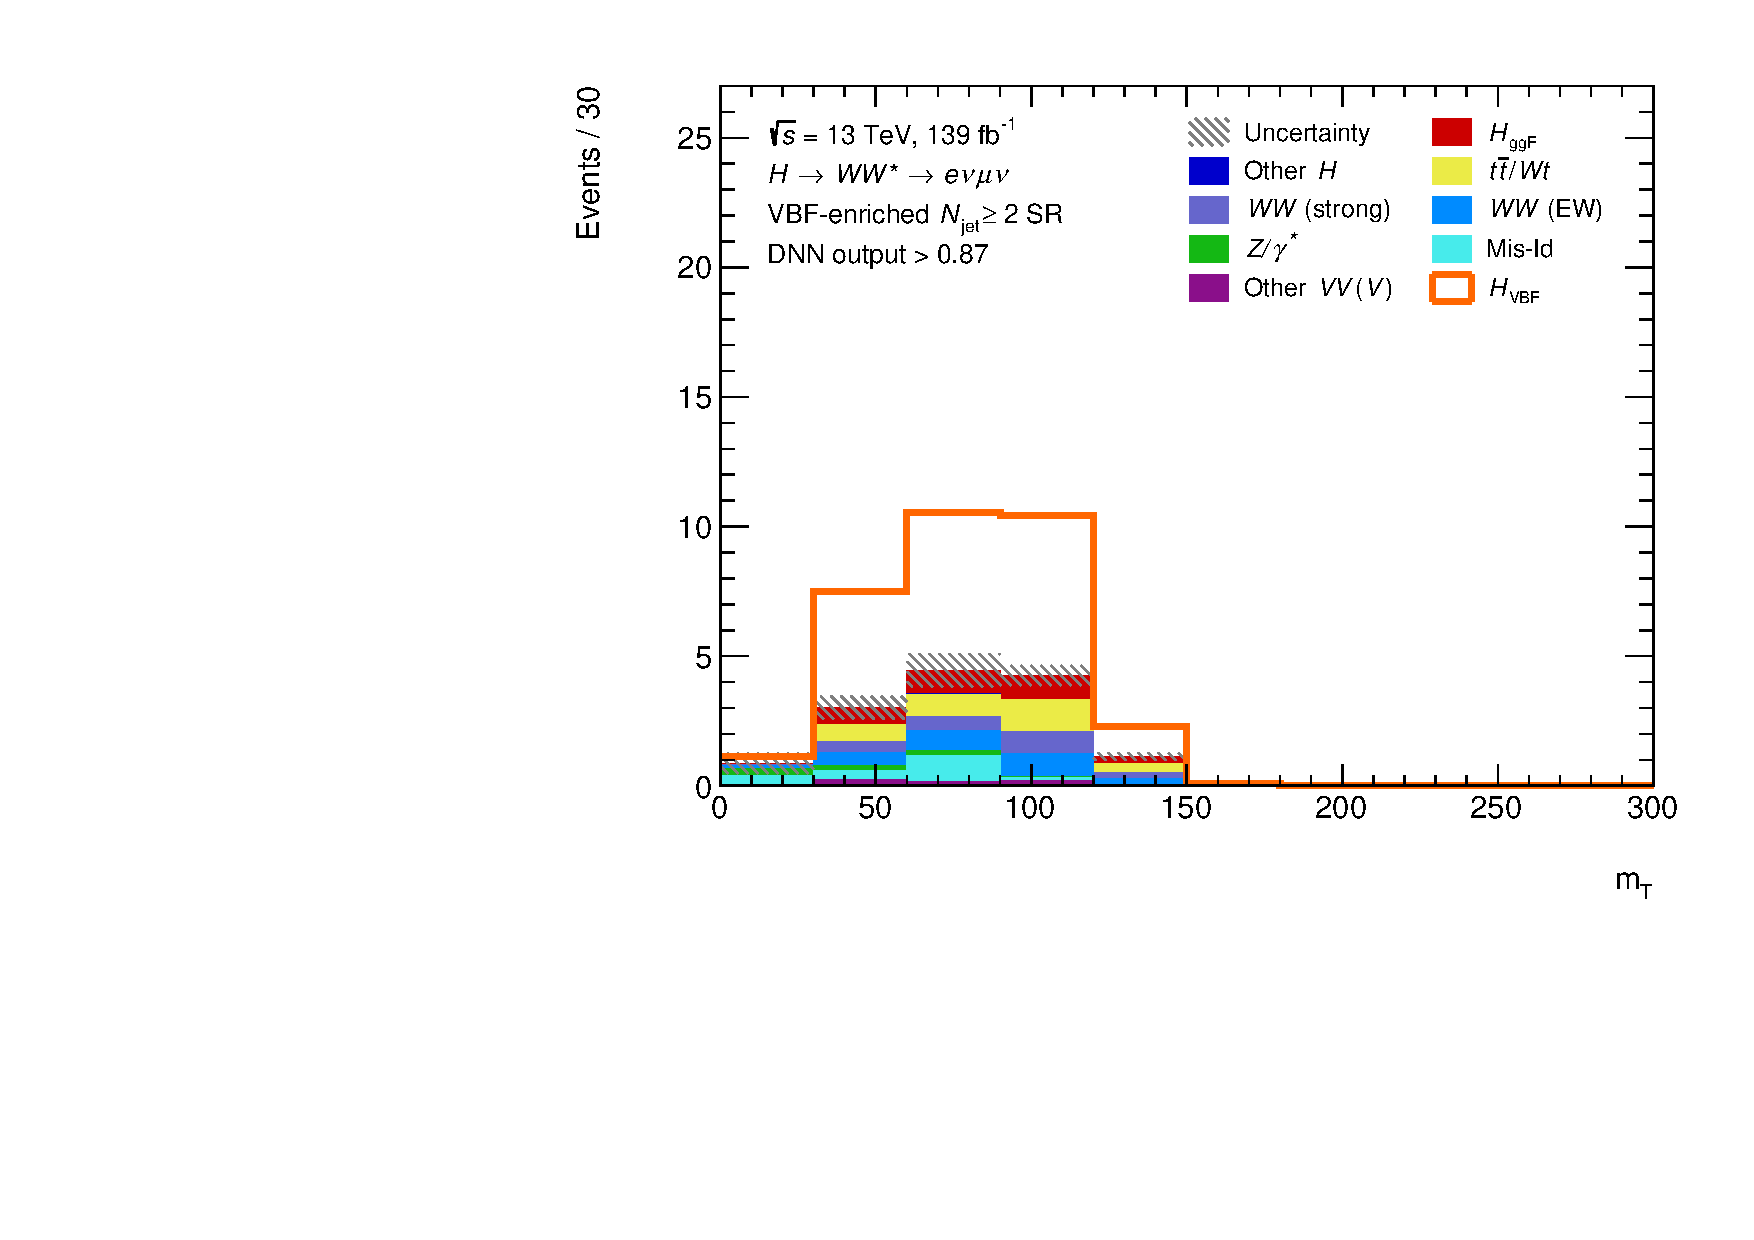
\includegraphics[width=0.32\textwidth]{figures/hww/dnn/blinded/run2-emme-CutVBFSR_DNN87-MT-lin.pdf}
    } \\
    \subfloat[$\pttot$]{
        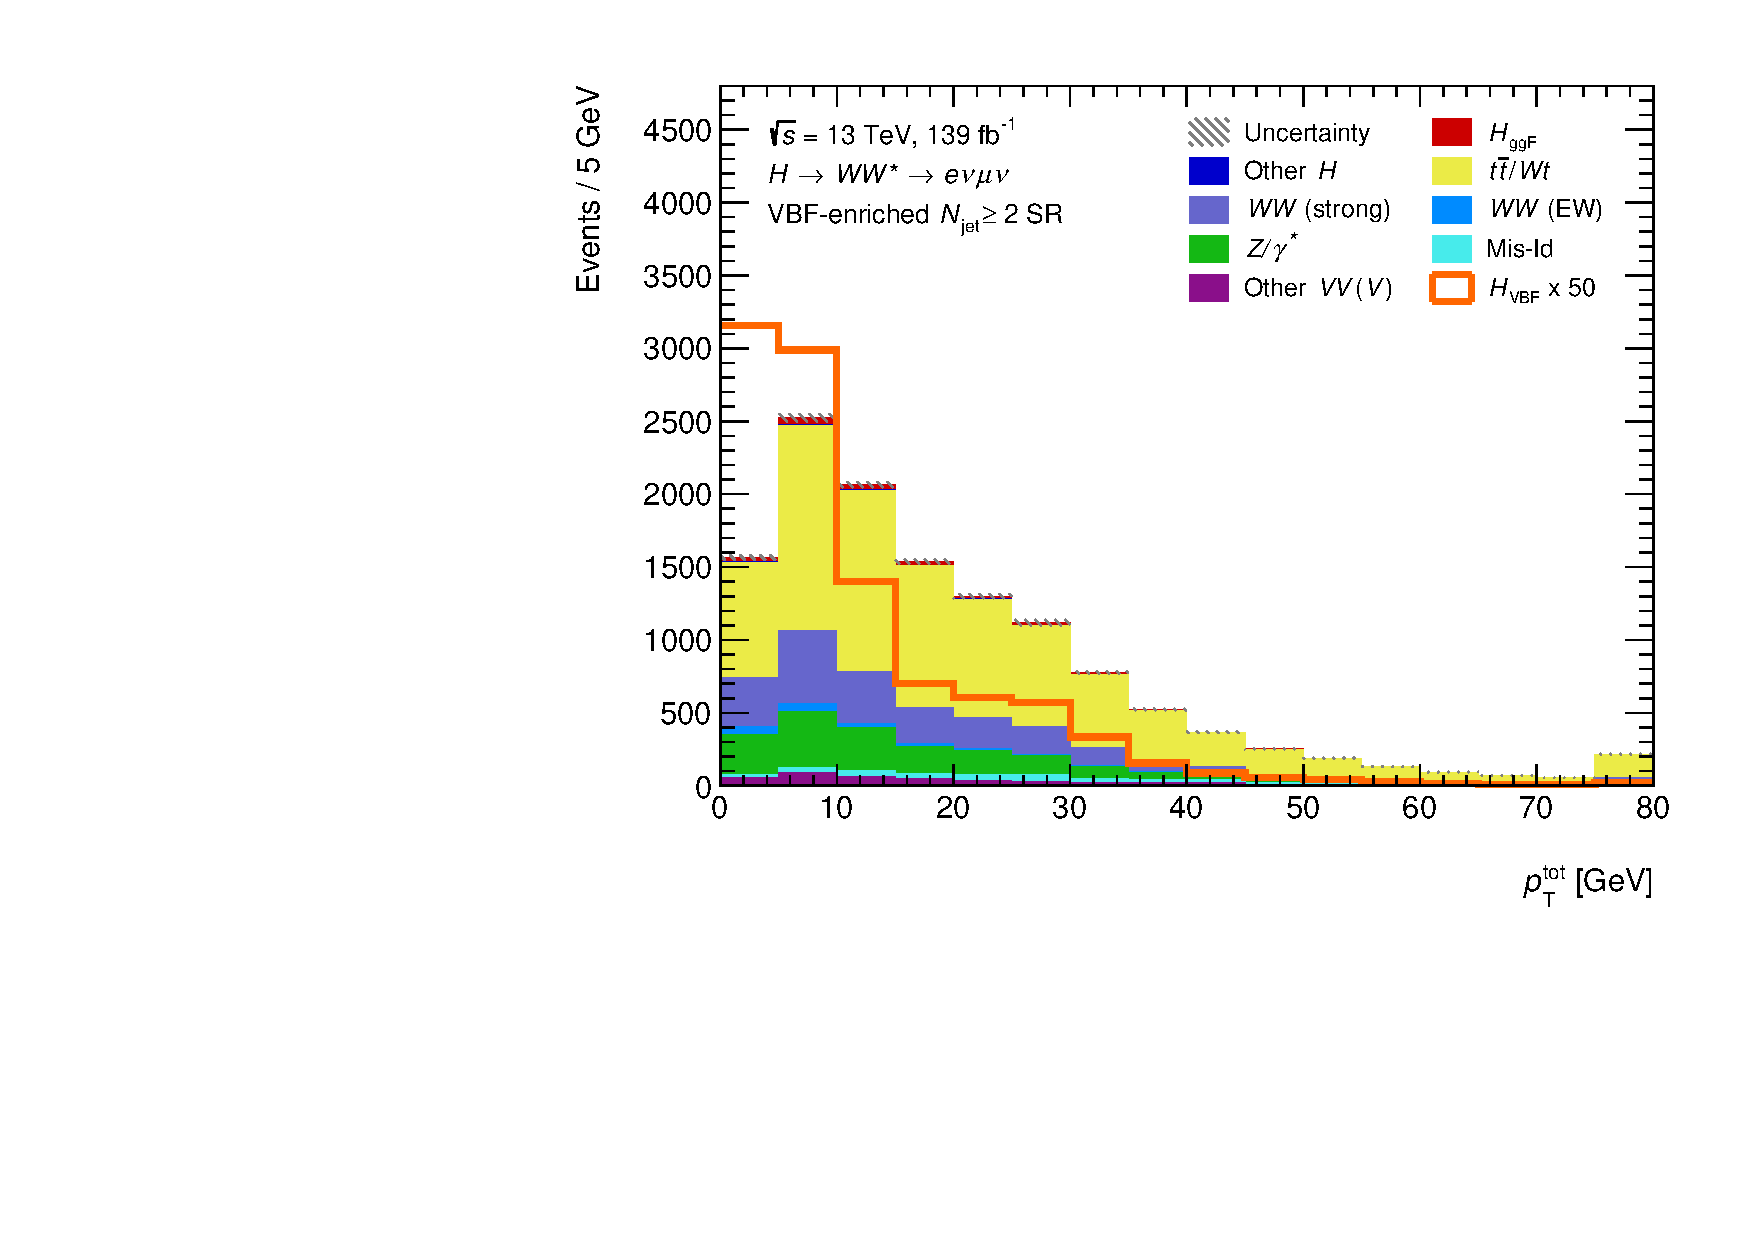
\includegraphics[width=0.32\textwidth]{figures/hww/dnn/blinded/run2-emme-CutVBF_SR-PtTot-lin.pdf} \hfill
        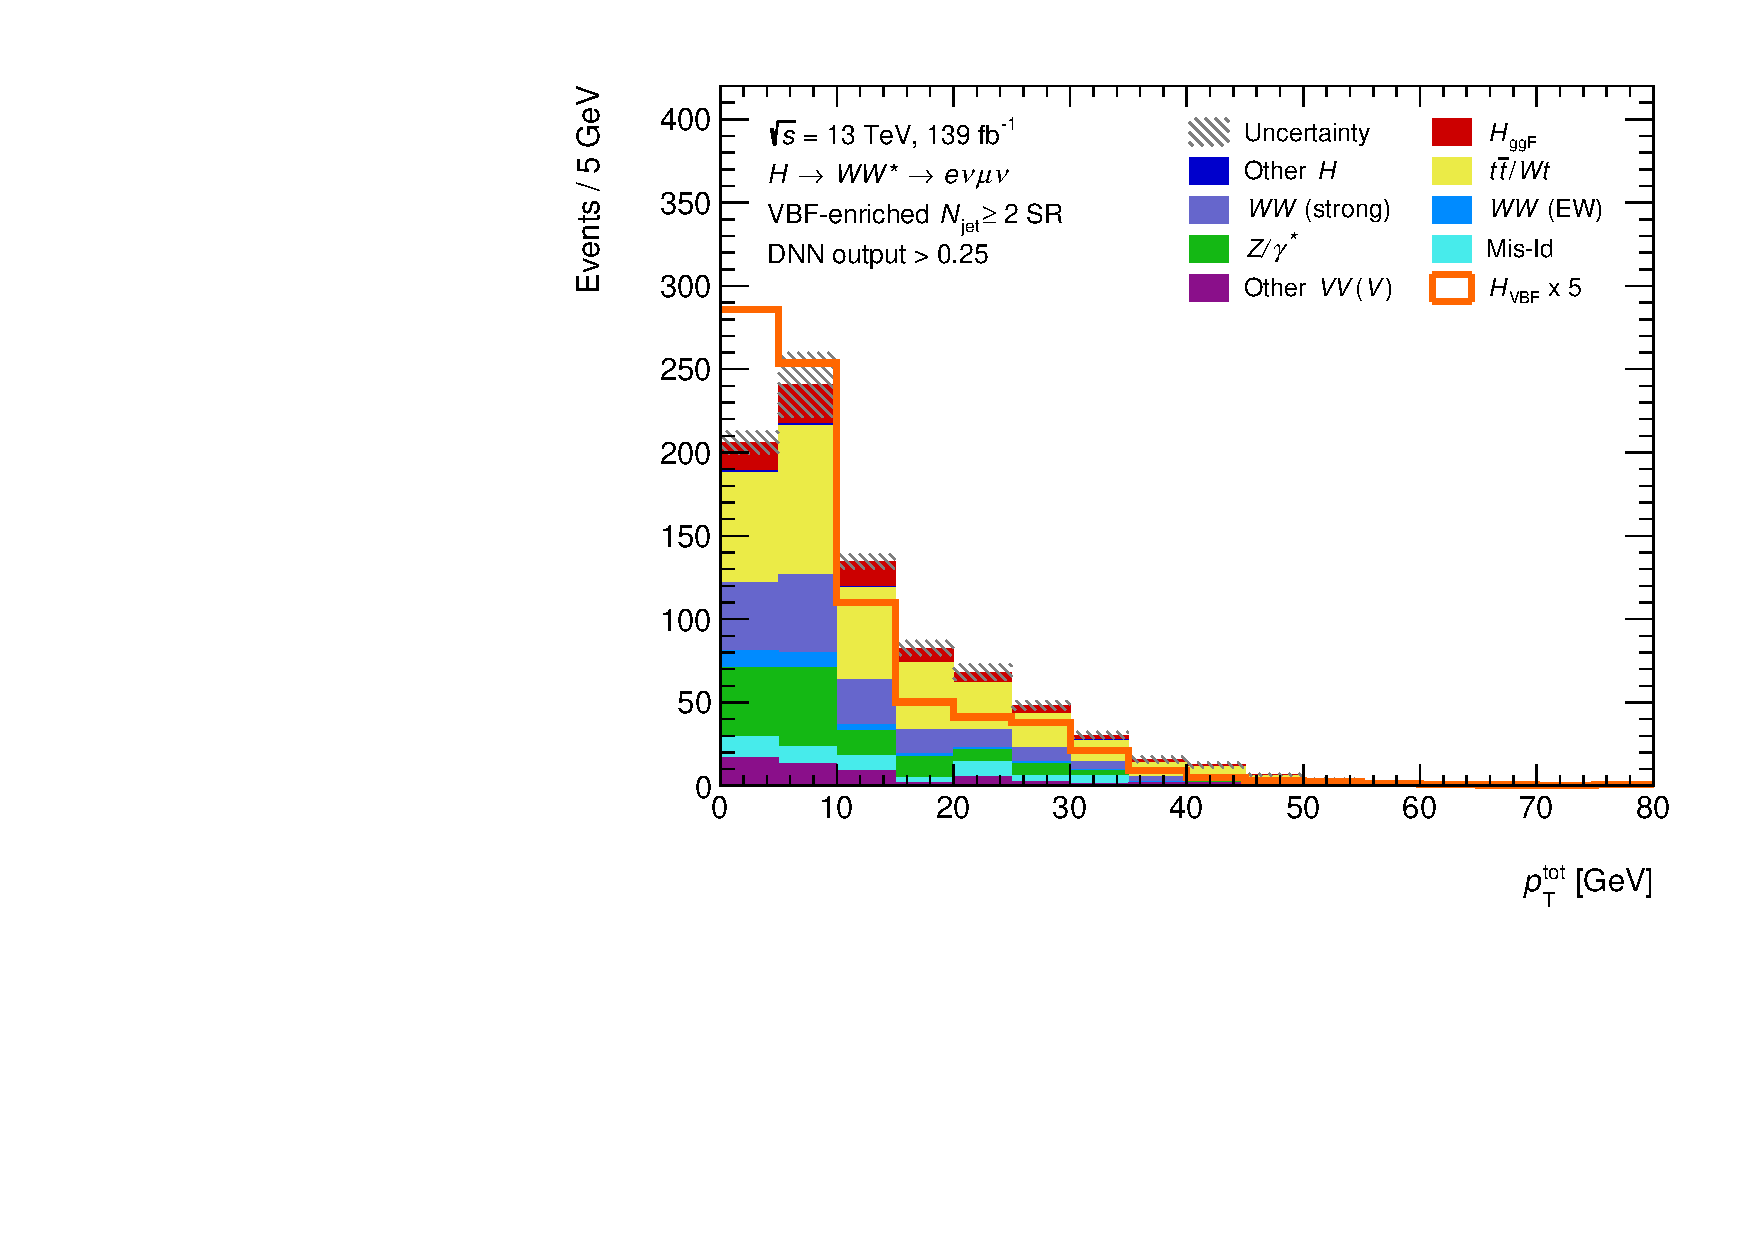
\includegraphics[width=0.32\textwidth]{figures/hww/dnn/blinded/run2-emme-CutVBFSR_DNN25-PtTot-lin.pdf} \hfill
        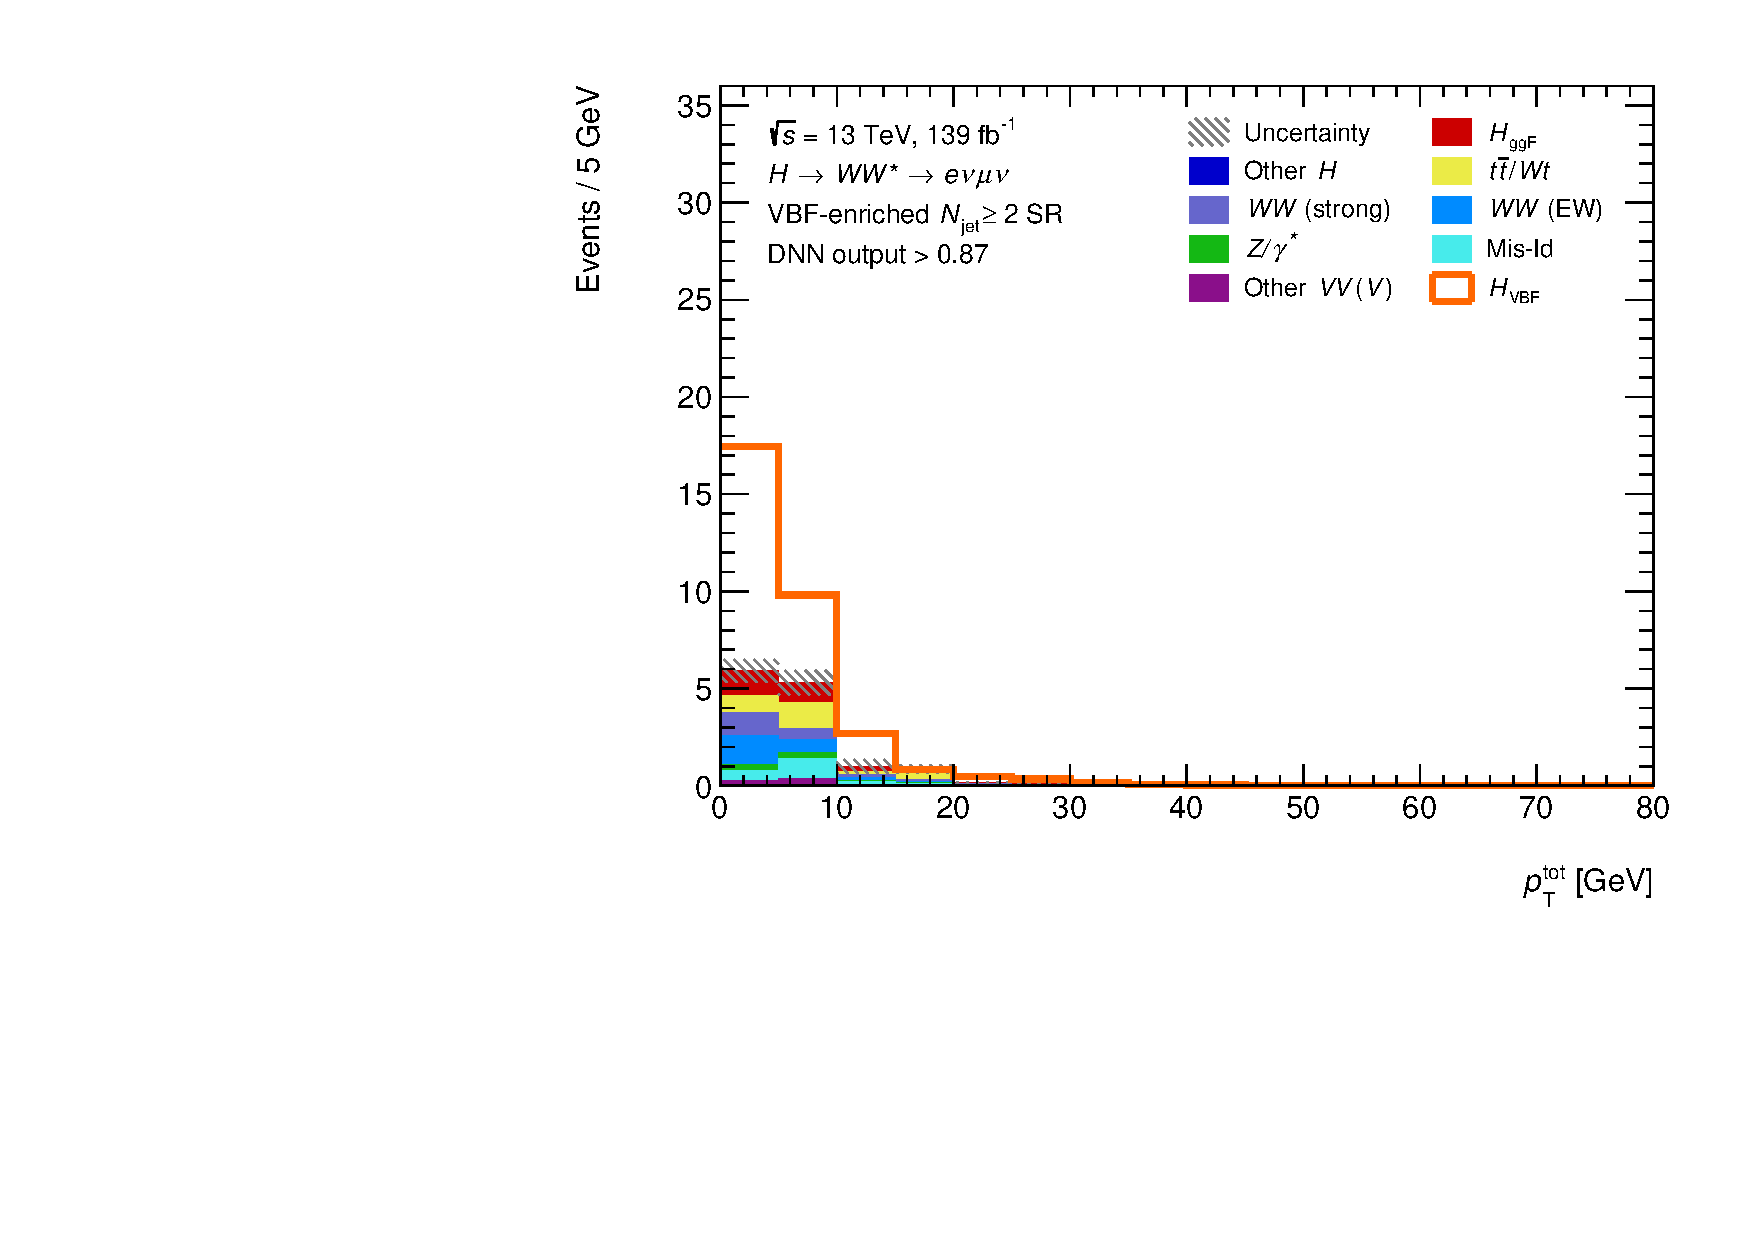
\includegraphics[width=0.32\textwidth]{figures/hww/dnn/blinded/run2-emme-CutVBFSR_DNN87-PtTot-lin.pdf}
    } \\
    \subfloat[$\lepetacent$]{
        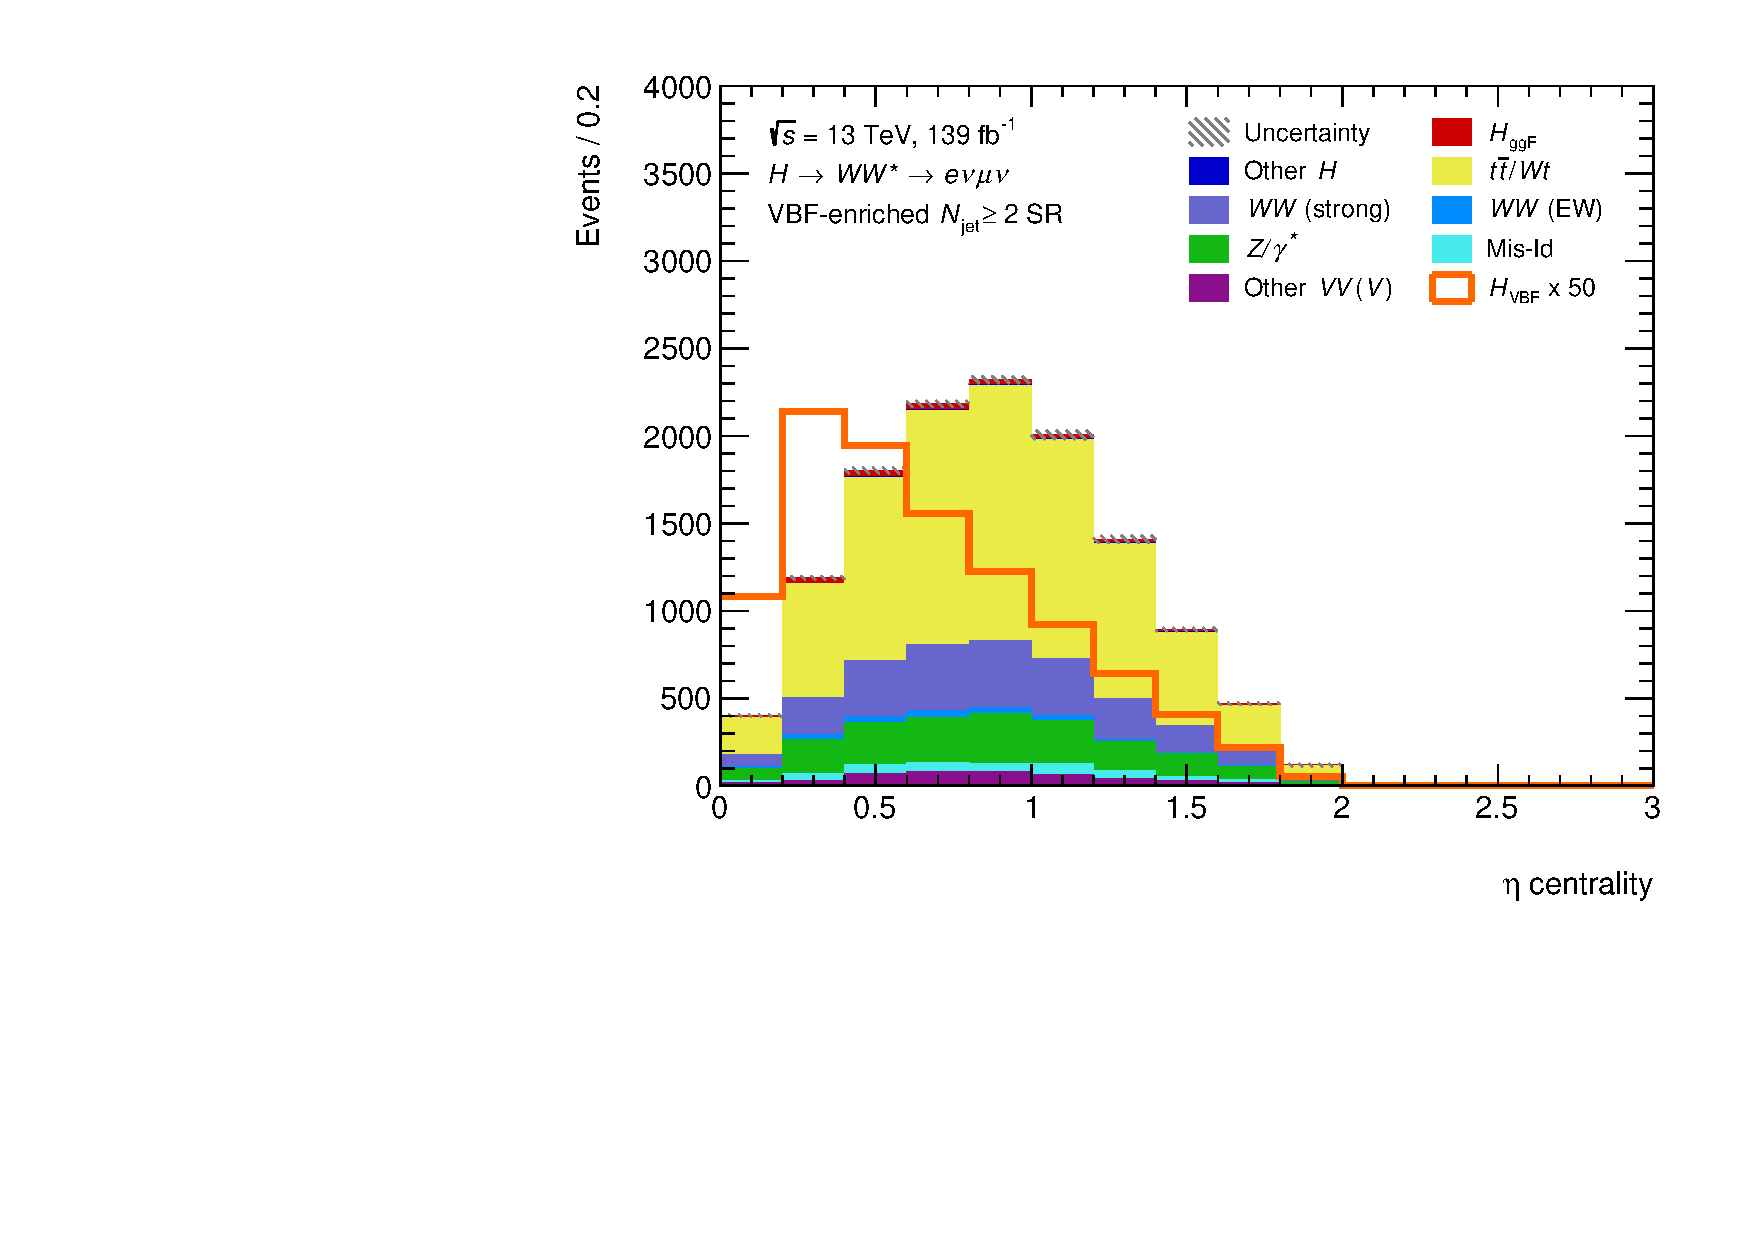
\includegraphics[width=0.32\textwidth]{figures/hww/dnn/blinded/run2-emme-CutVBF_SR-contOLV-lin.pdf} \hfill
        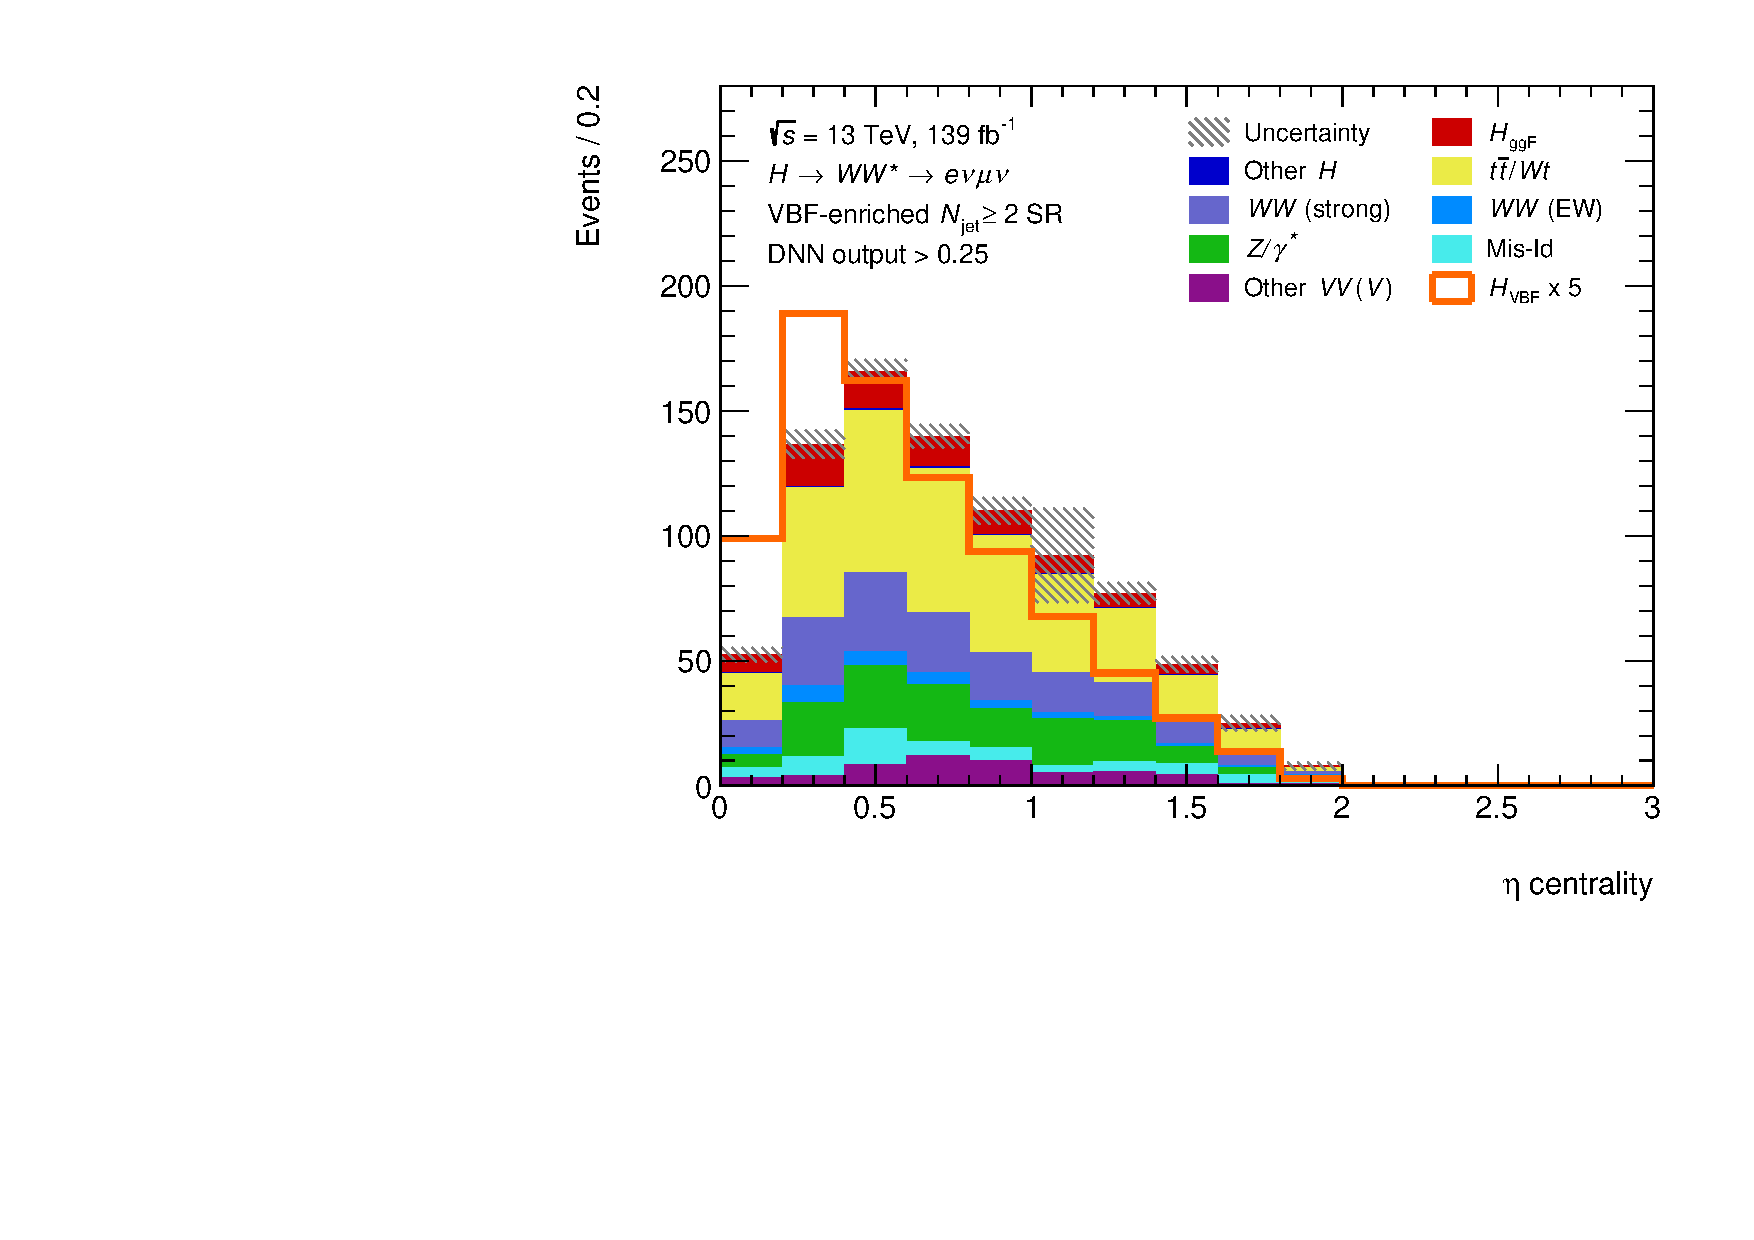
\includegraphics[width=0.32\textwidth]{figures/hww/dnn/blinded/run2-emme-CutVBFSR_DNN25-contOLV-lin.pdf} \hfill
        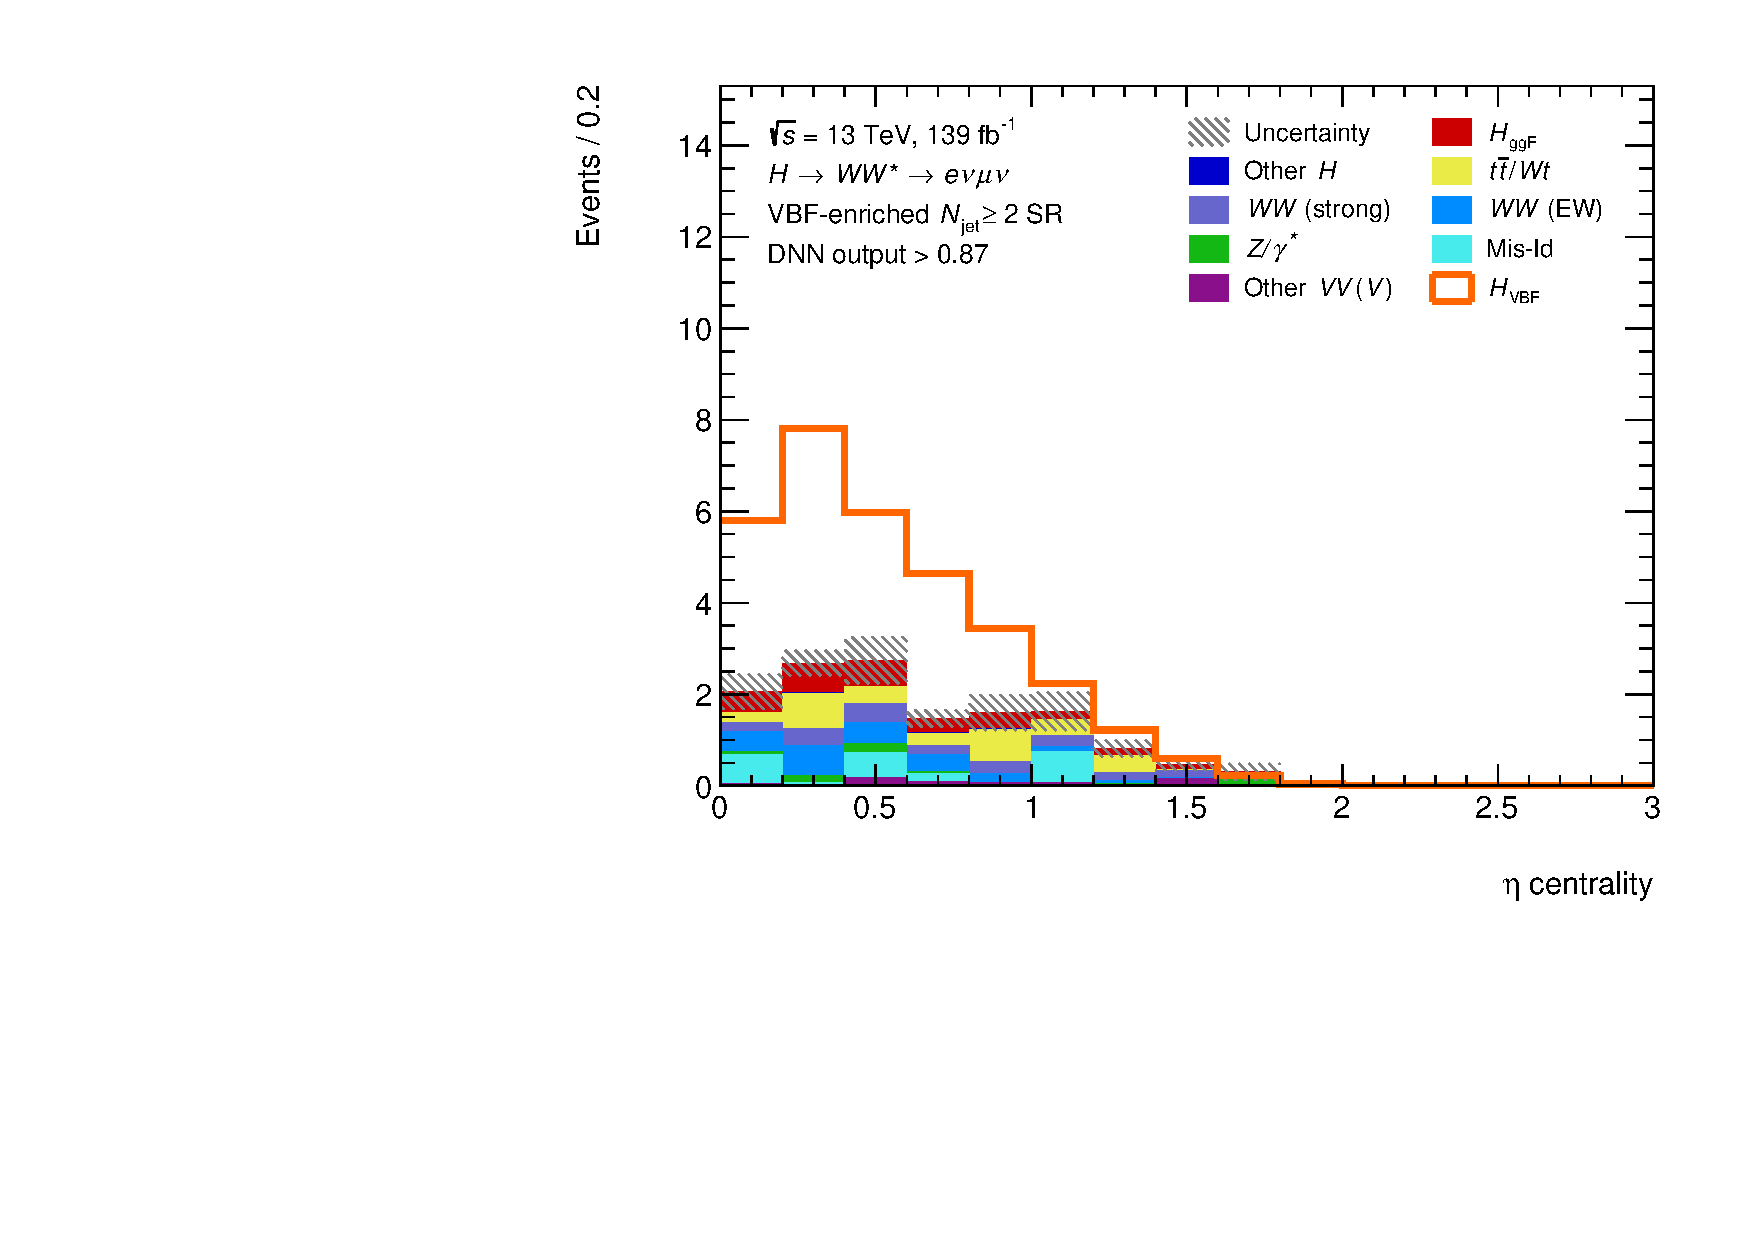
\includegraphics[width=0.32\textwidth]{figures/hww/dnn/blinded/run2-emme-CutVBFSR_DNN87-contOLV-lin.pdf}
    } \\
    \subfloat[$\METSig$]{
        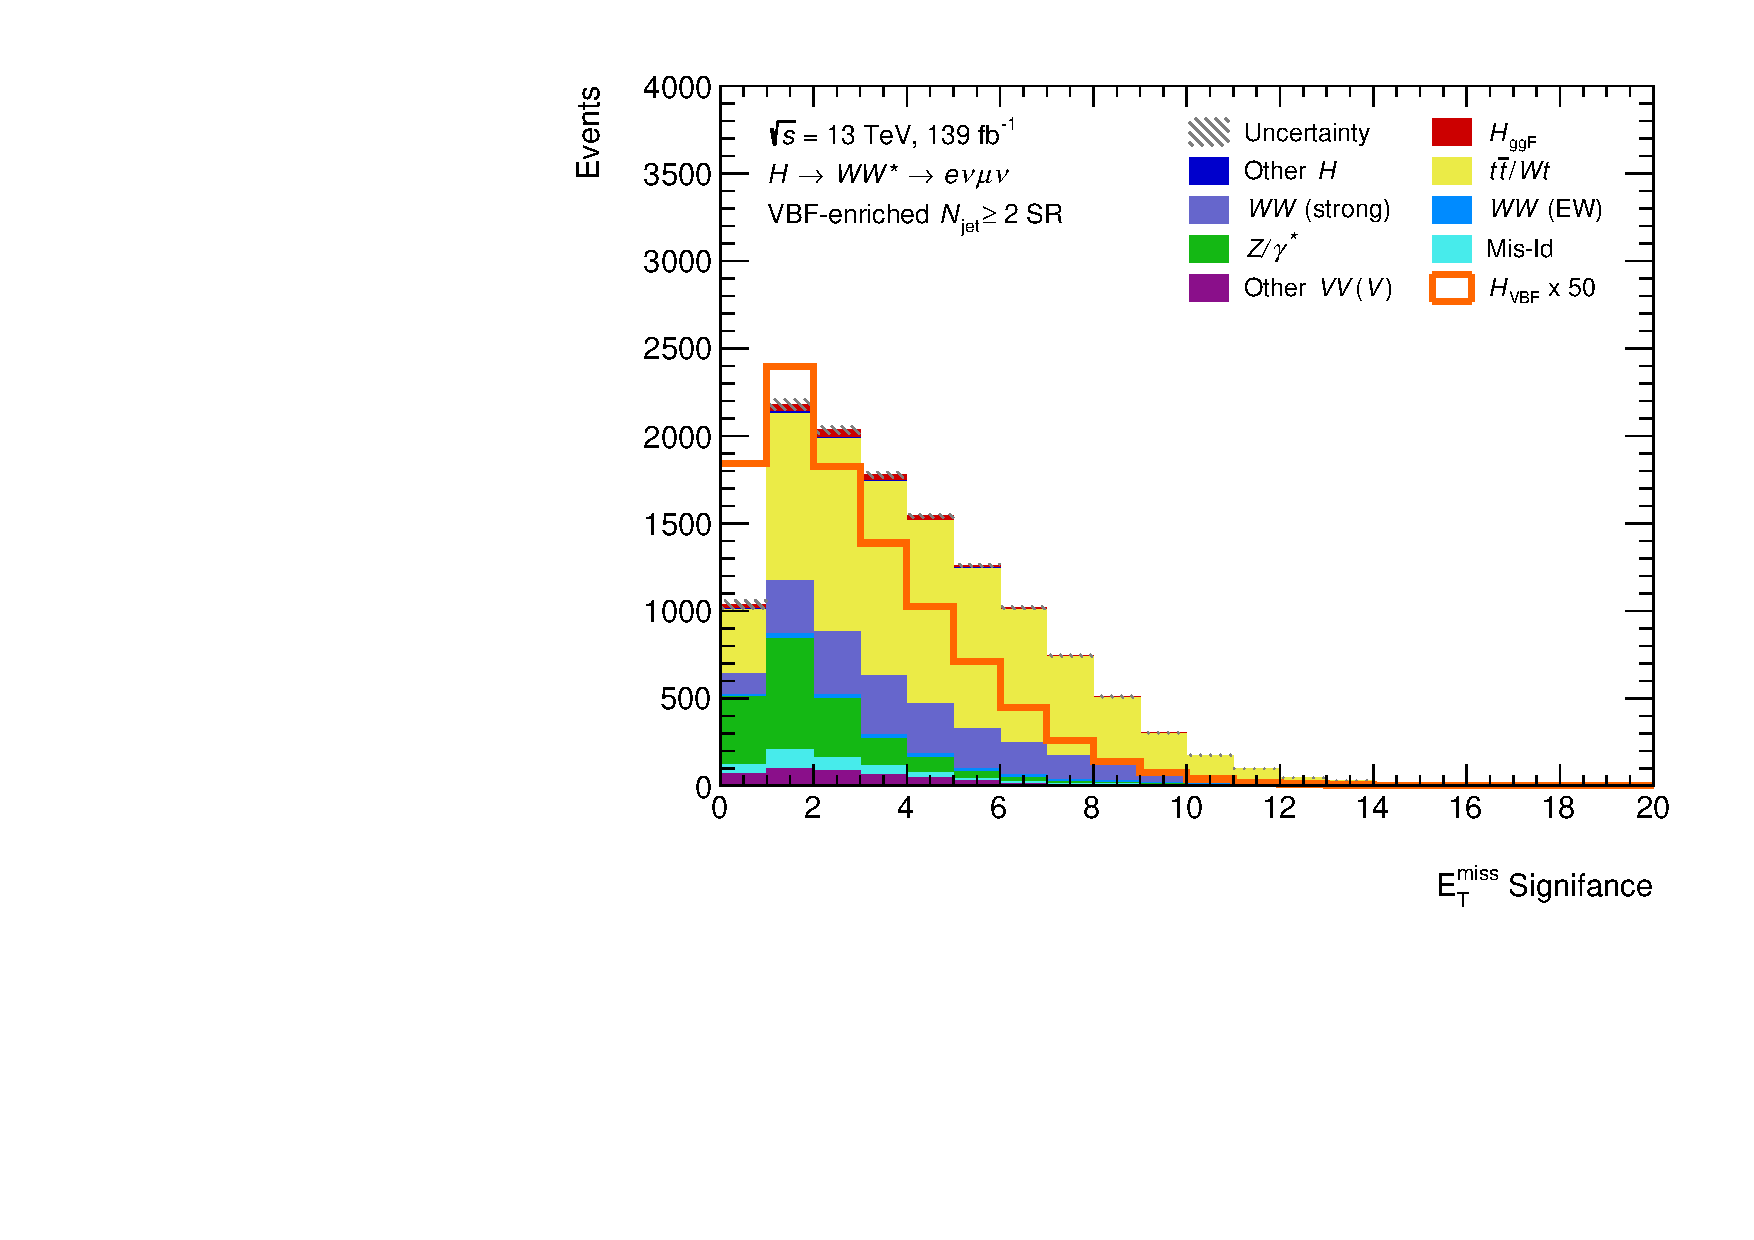
\includegraphics[width=0.32\textwidth]{figures/hww/dnn/blinded/run2-emme-CutVBF_SR-METSig_broad-lin.pdf} \hfill
        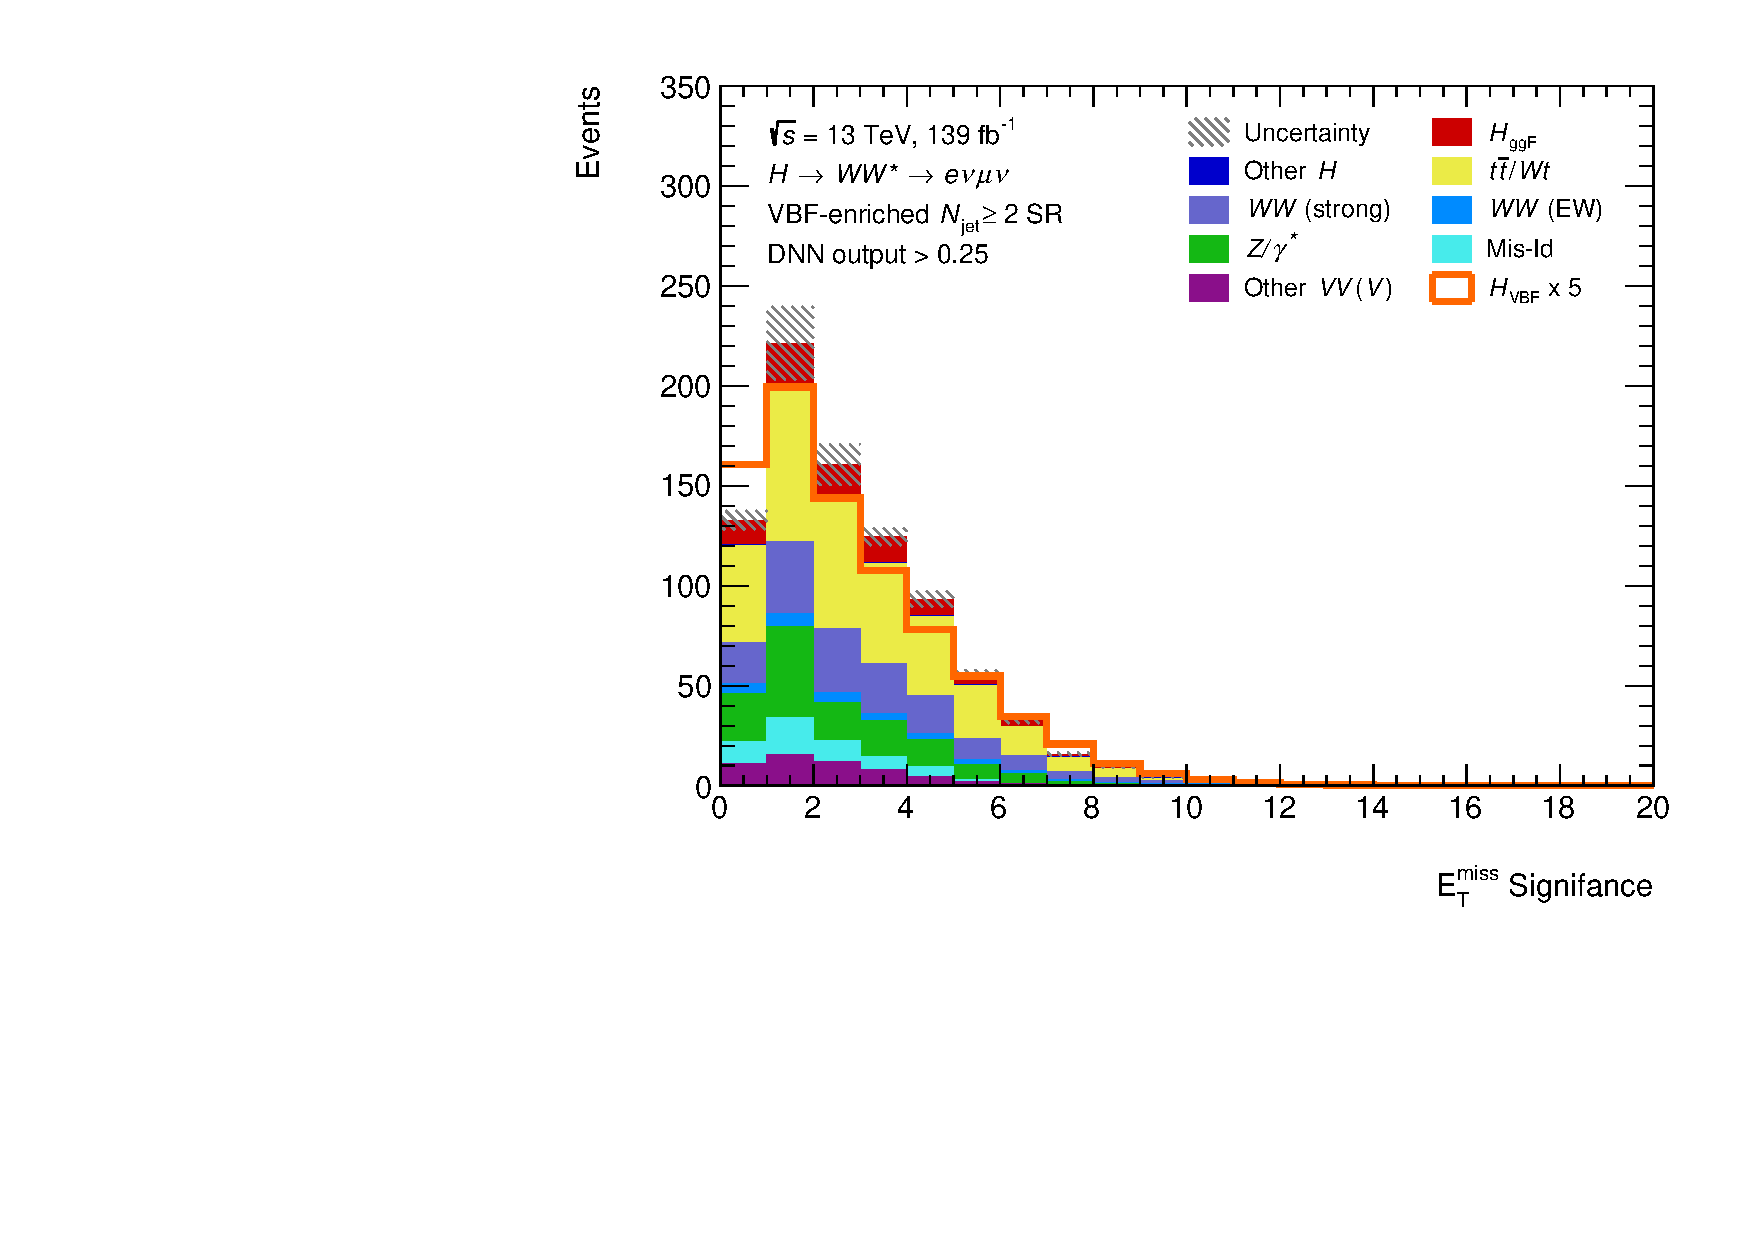
\includegraphics[width=0.32\textwidth]{figures/hww/dnn/blinded/run2-emme-CutVBFSR_DNN25-METSig_broad-lin.pdf} \hfill
        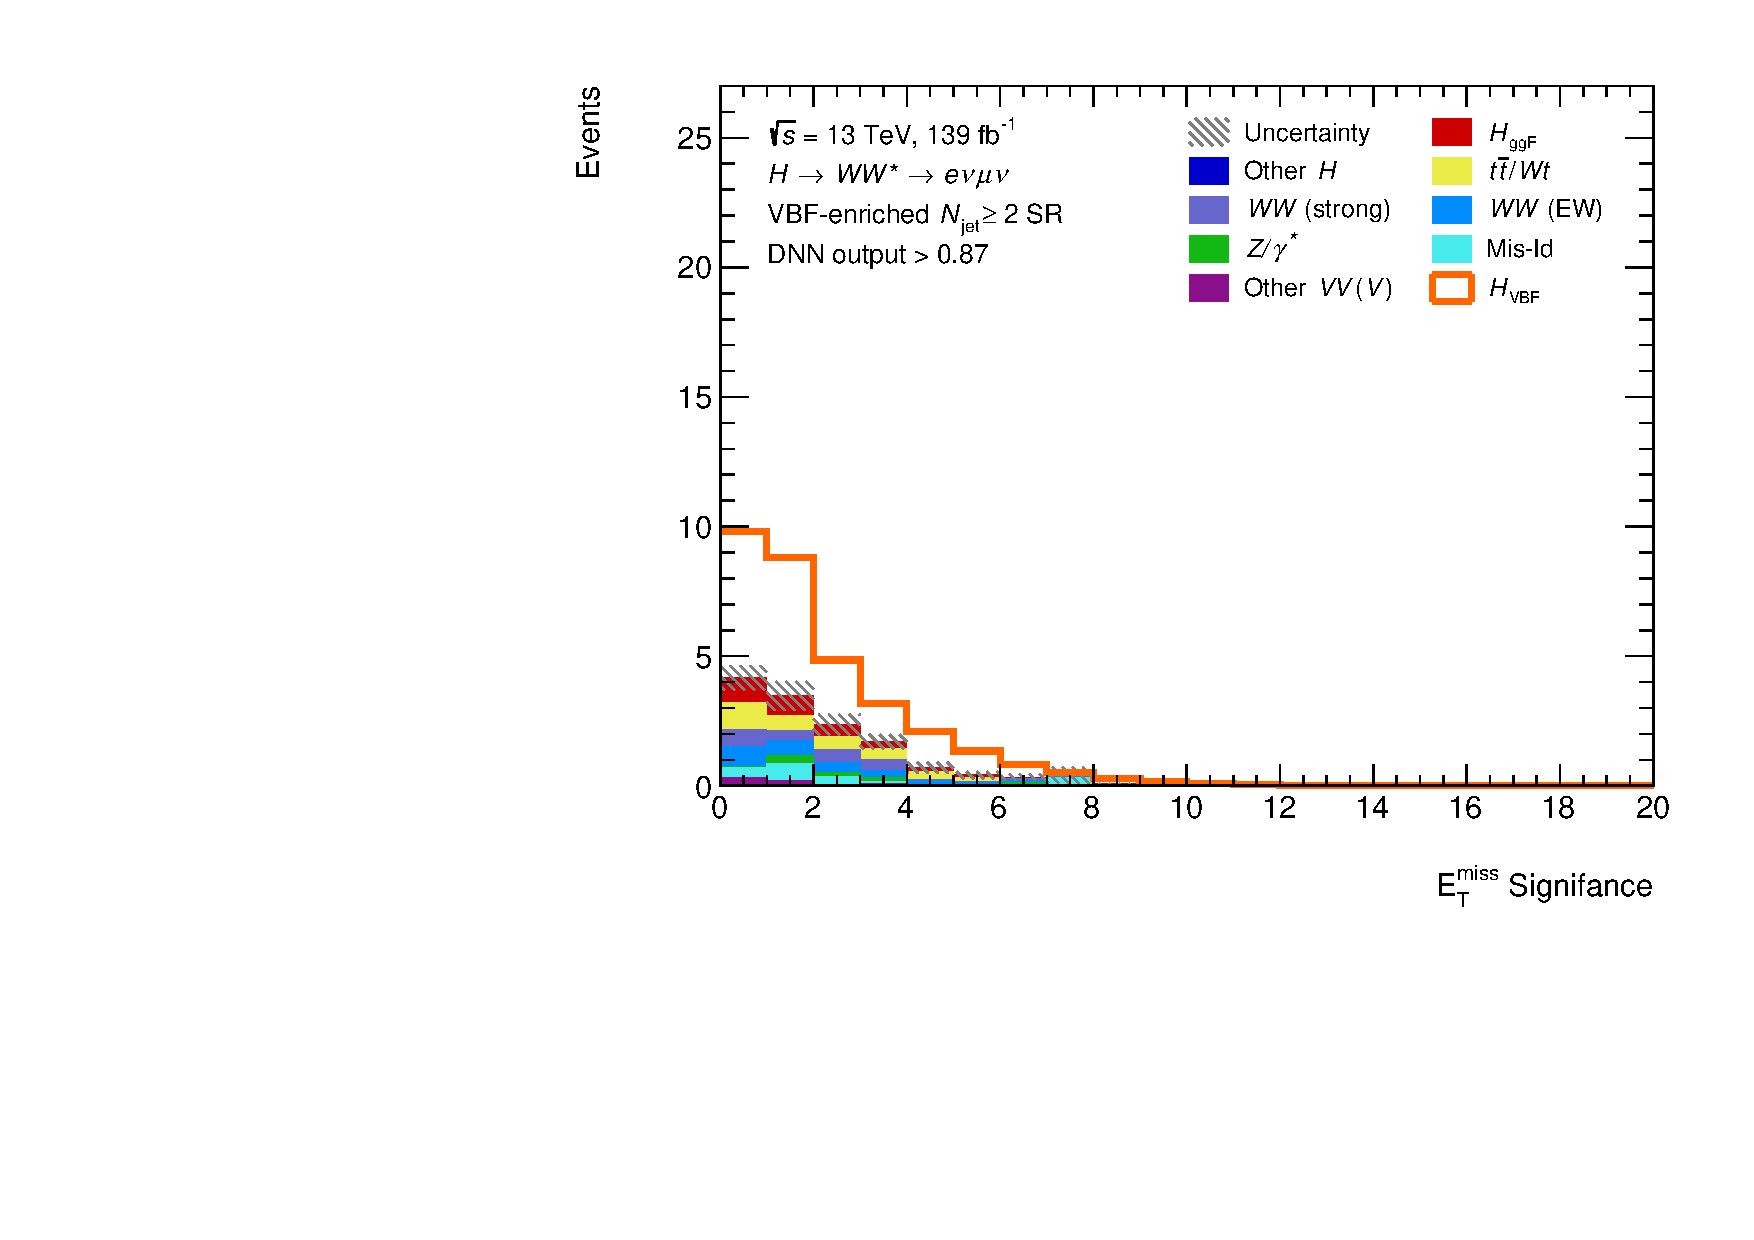
\includegraphics[width=0.32\textwidth]{figures/hww/dnn/blinded/run2-emme-CutVBFSR_DNN87-METSig_broad-lin.pdf}
    } \\
    {\caption{Distributions of $\mT$, $\pttot$, $\lepetacent$, $\METSig$ in the VBF signal region.
            Each row shows one variable with different cuts on the DNN output distribution being applied in different columns.
            \label{fig:vbf:blindedSR1} }}
\end{figure}



\begin{figure}[h]
    \centering
    \subfloat[$\pTjone$]{
        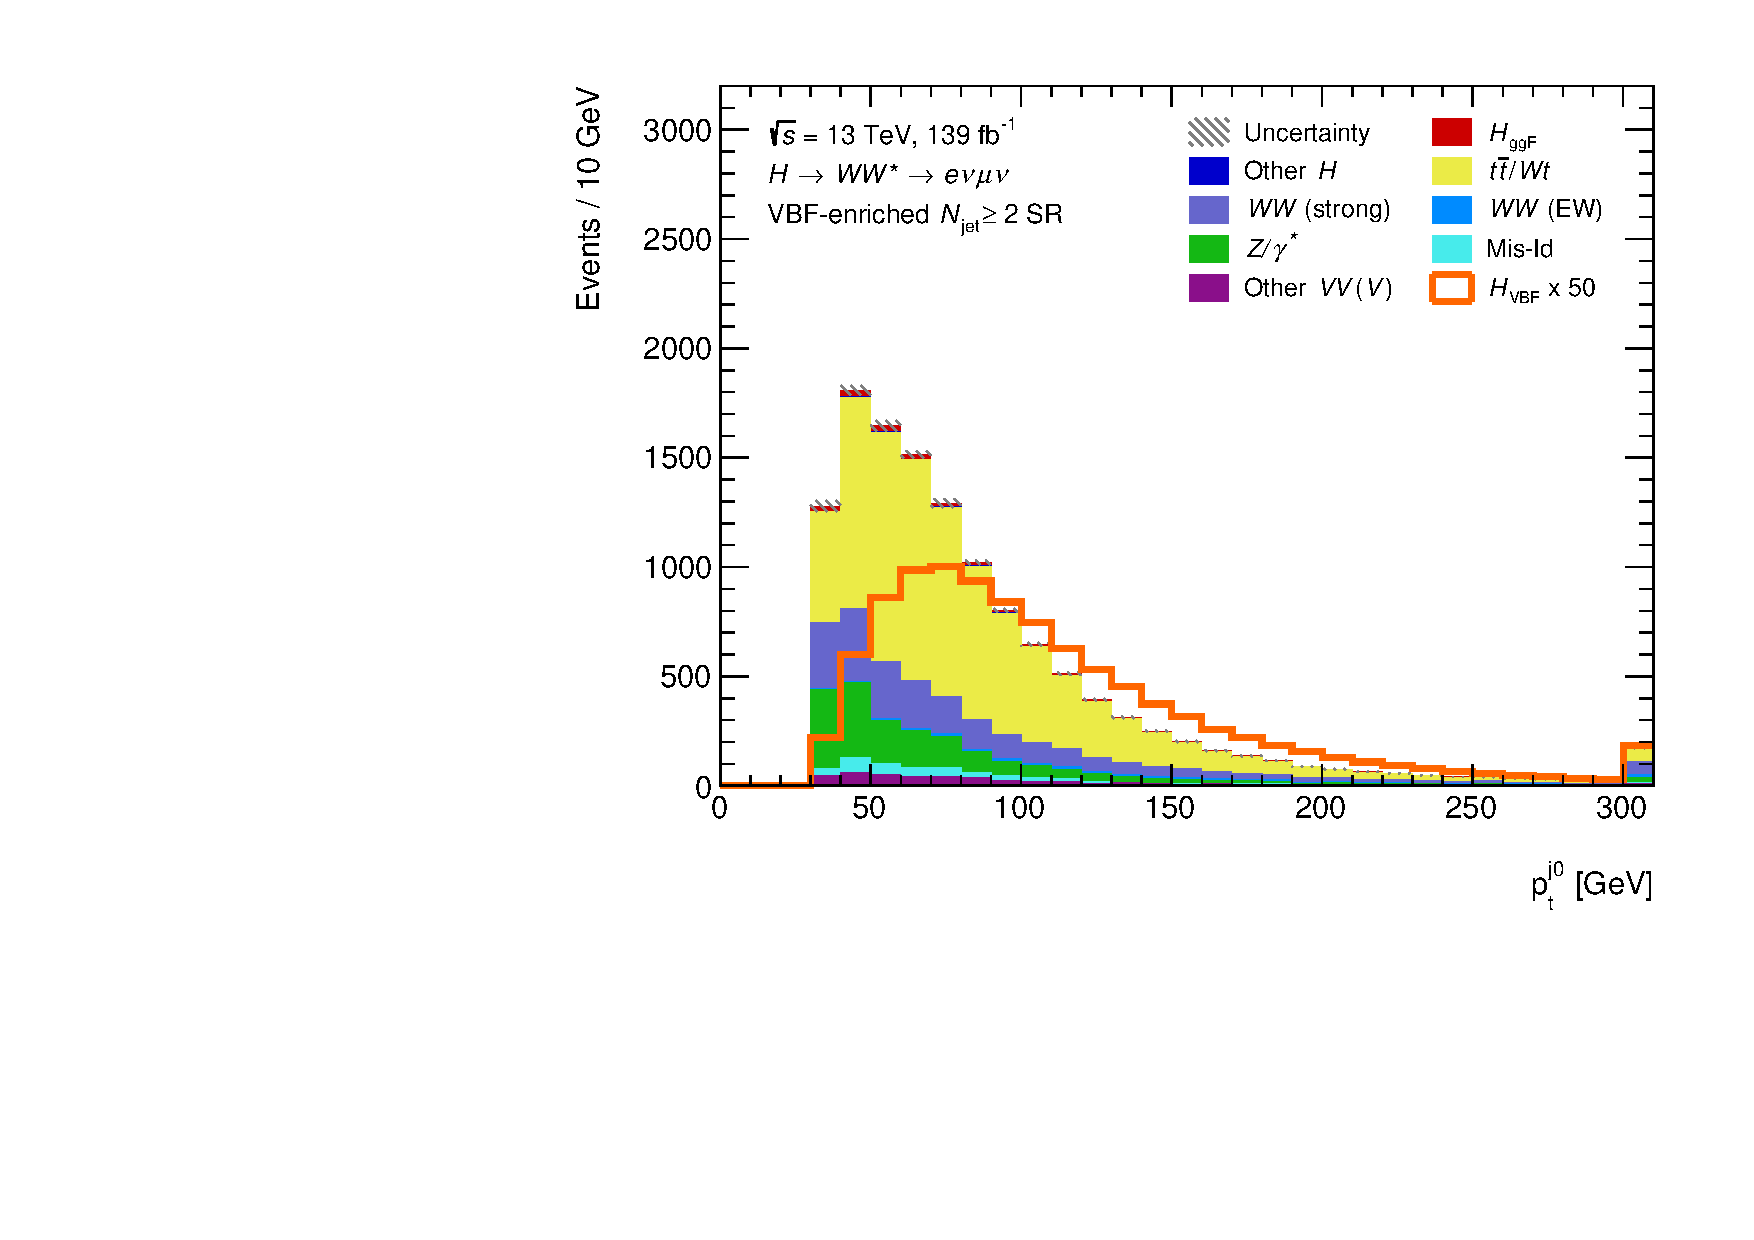
\includegraphics[width=0.32\textwidth]{figures/hww/dnn/blinded/run2-emme-CutVBF_SR-leadJetPt-lin.pdf} \hfill
        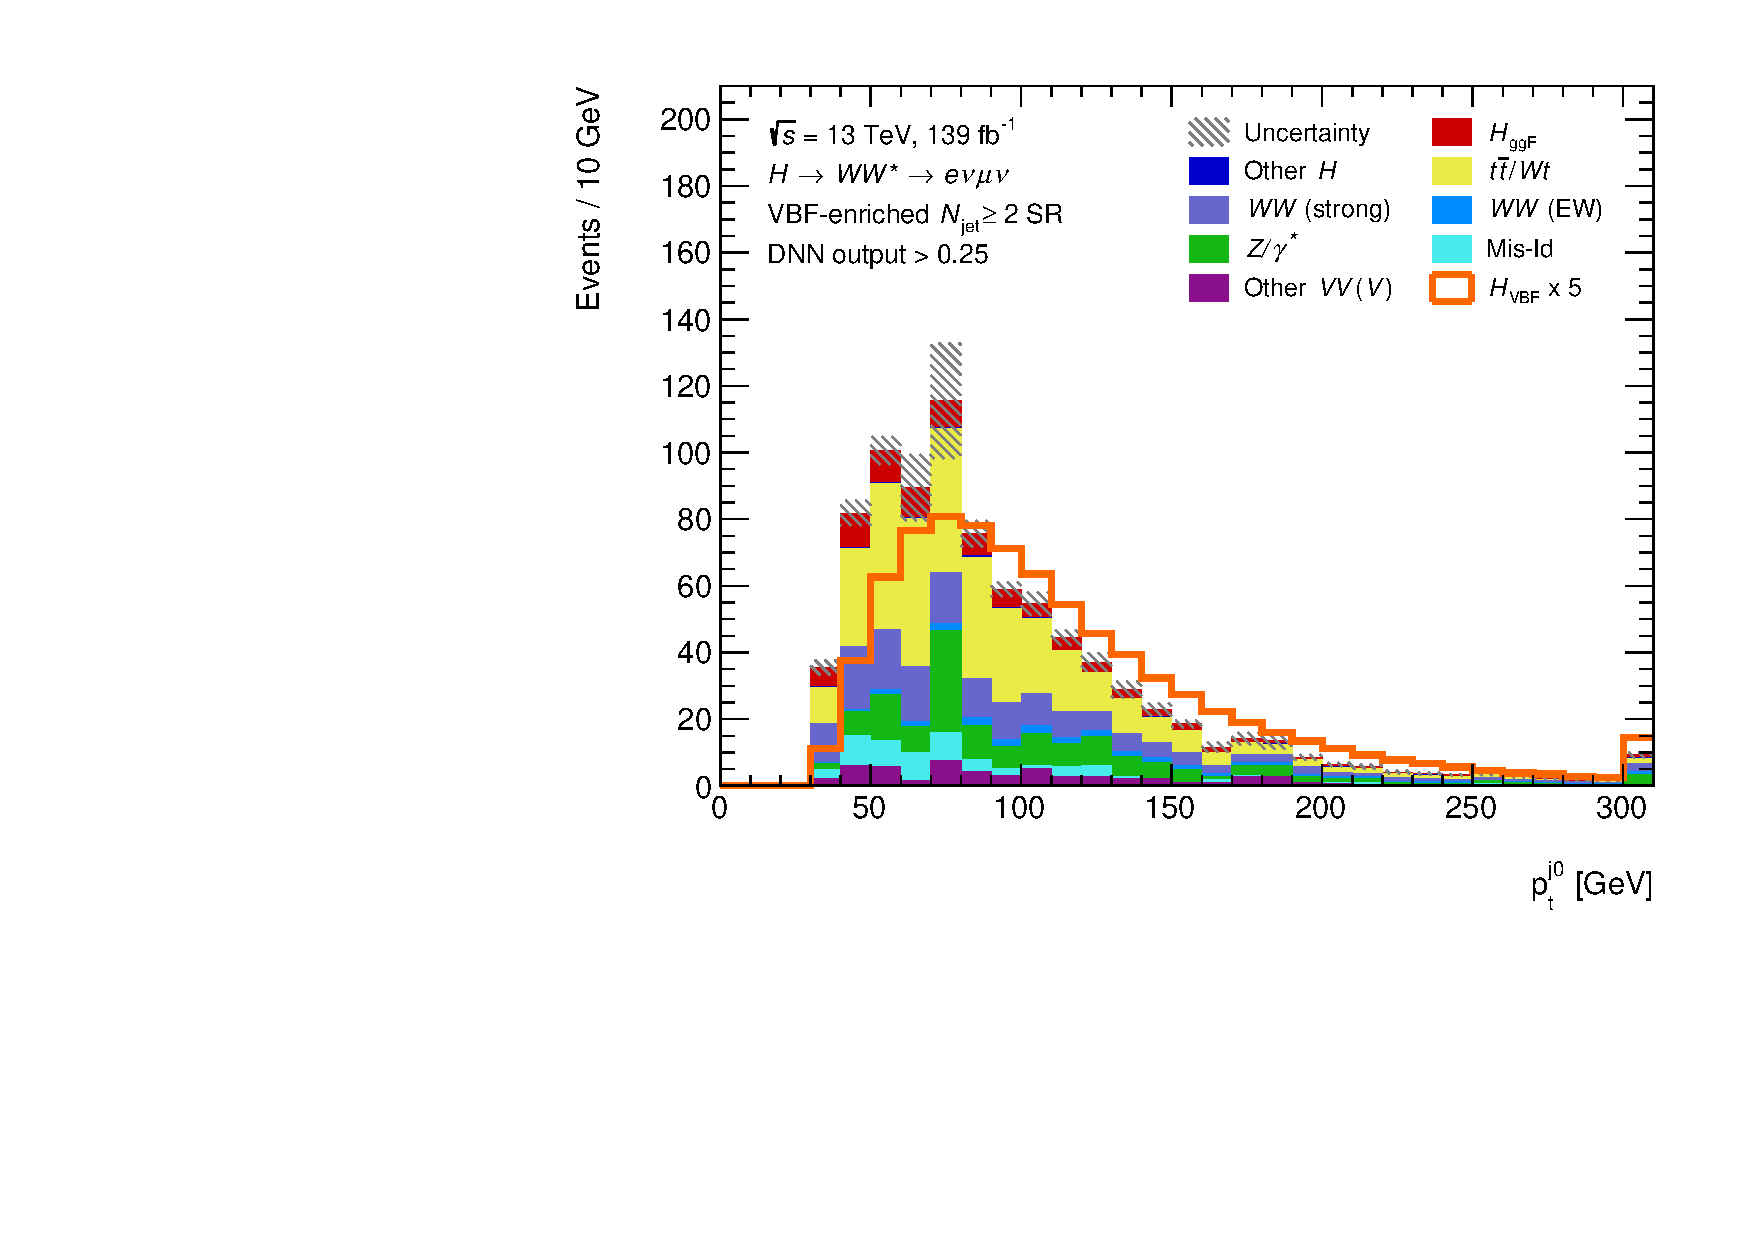
\includegraphics[width=0.32\textwidth]{figures/hww/dnn/blinded/run2-emme-CutVBFSR_DNN25-leadJetPt-lin.pdf} \hfill
        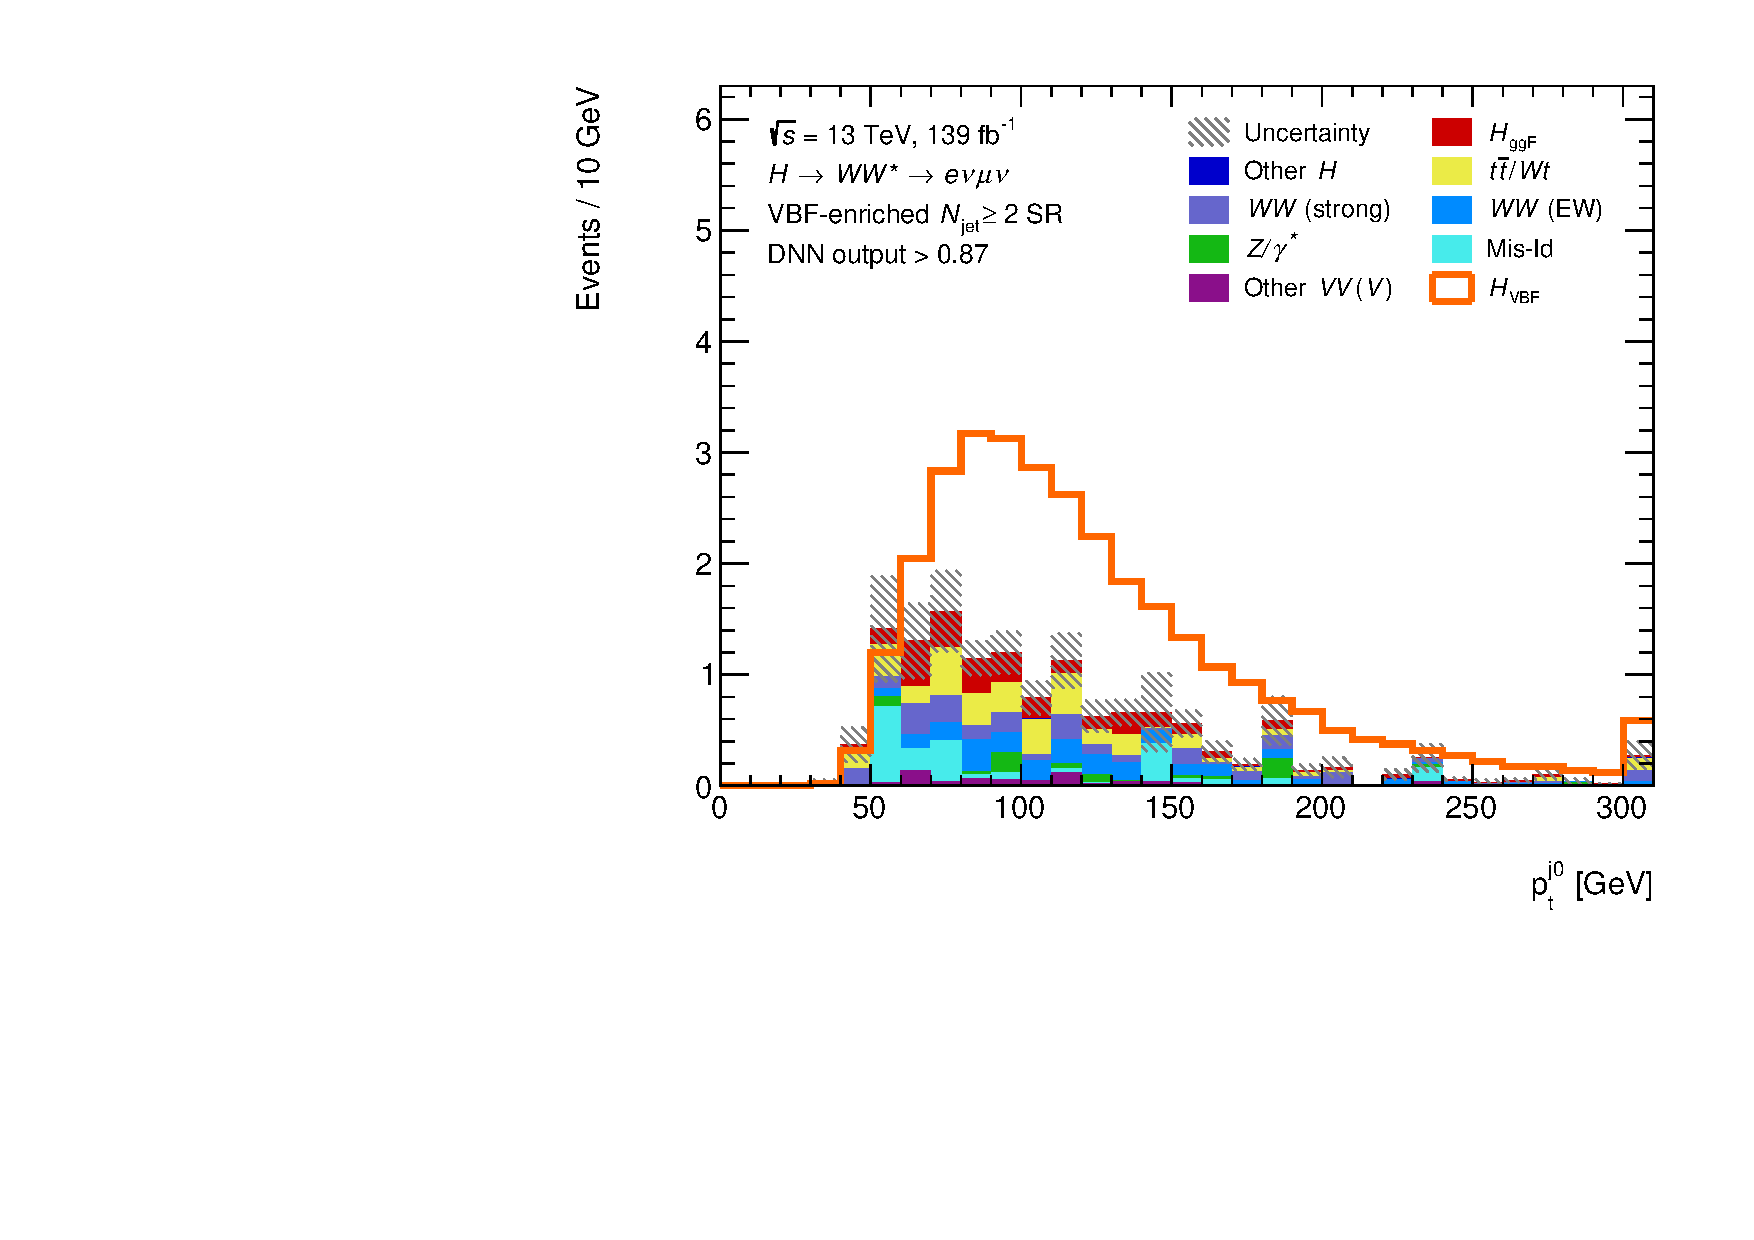
\includegraphics[width=0.32\textwidth]{figures/hww/dnn/blinded/run2-emme-CutVBFSR_DNN87-leadJetPt-lin.pdf}
    } \\
    \subfloat[$\pTjtwo$]{
        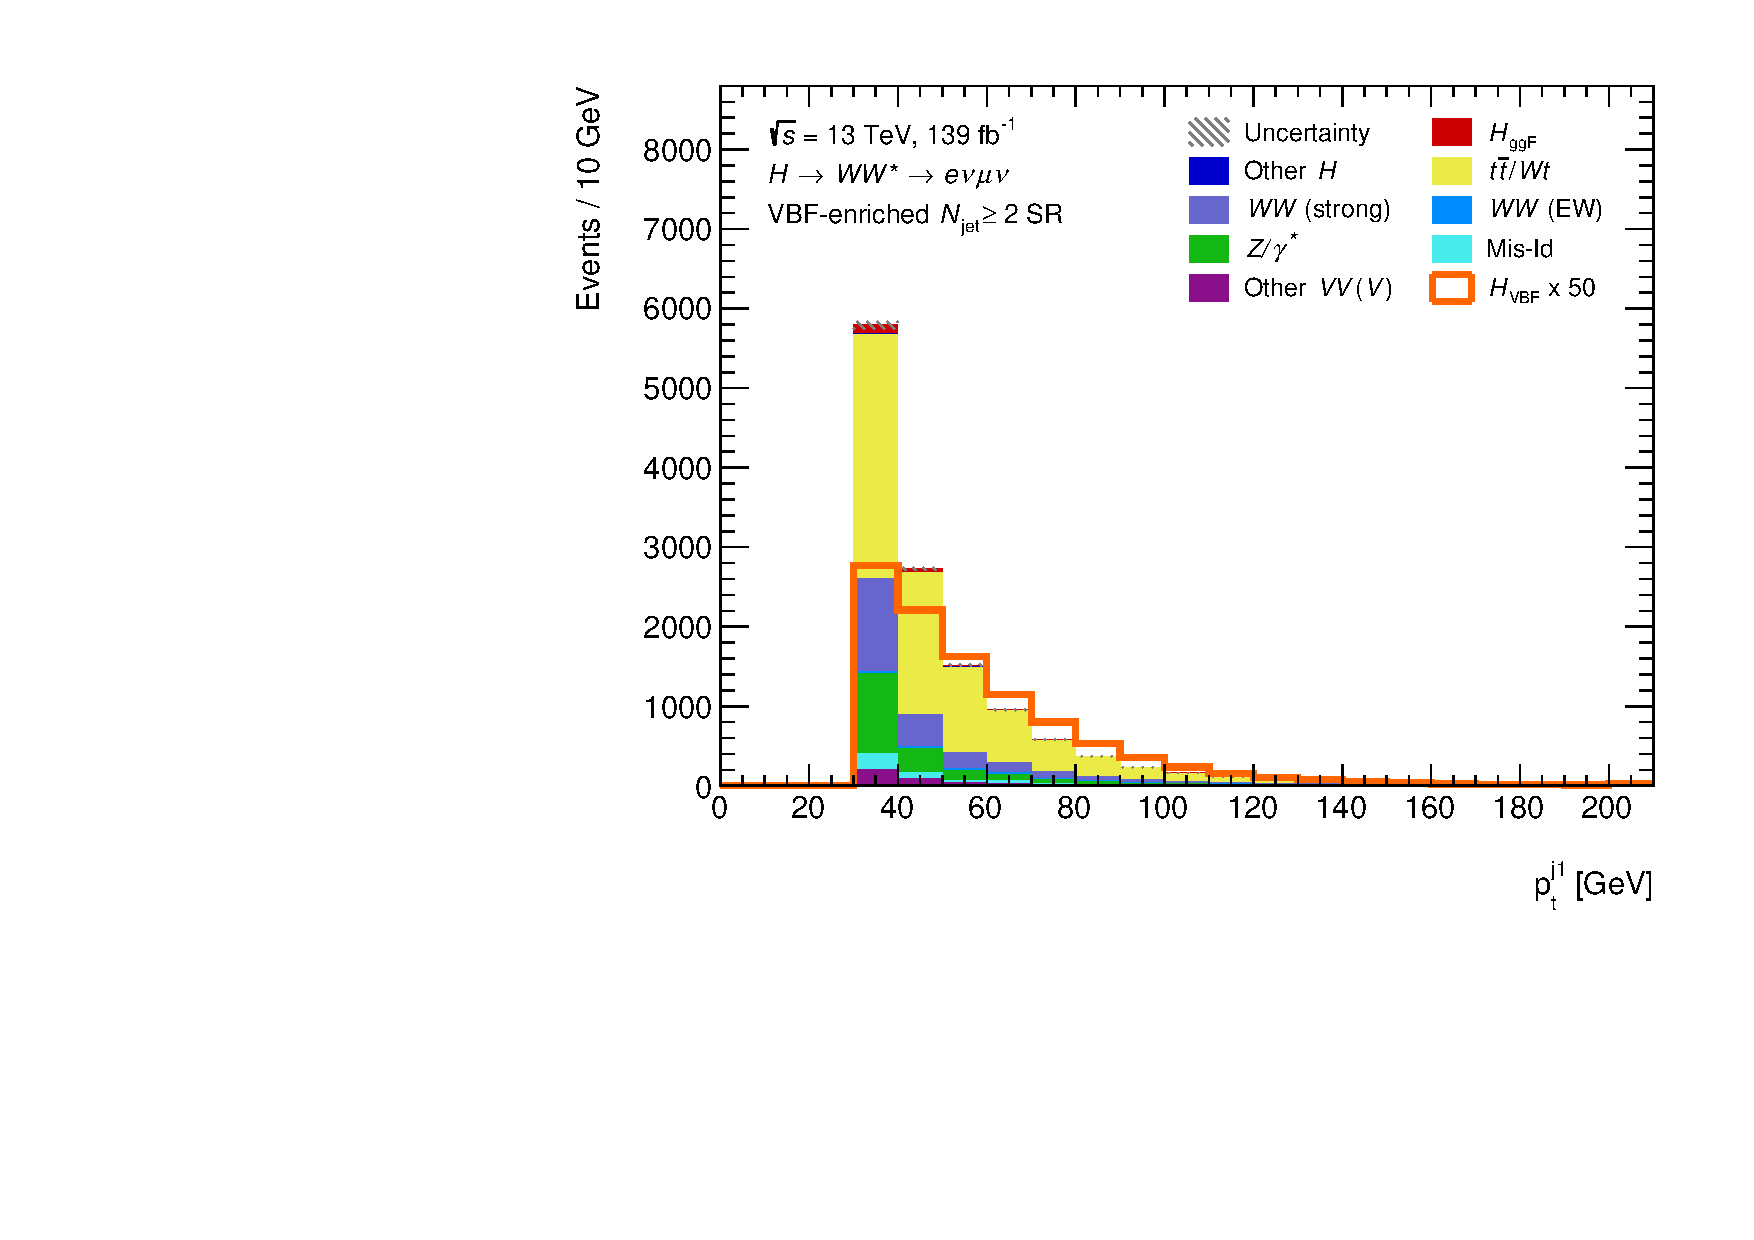
\includegraphics[width=0.32\textwidth]{figures/hww/dnn/blinded/run2-emme-CutVBF_SR-subleadJetPt-lin.pdf} \hfill
        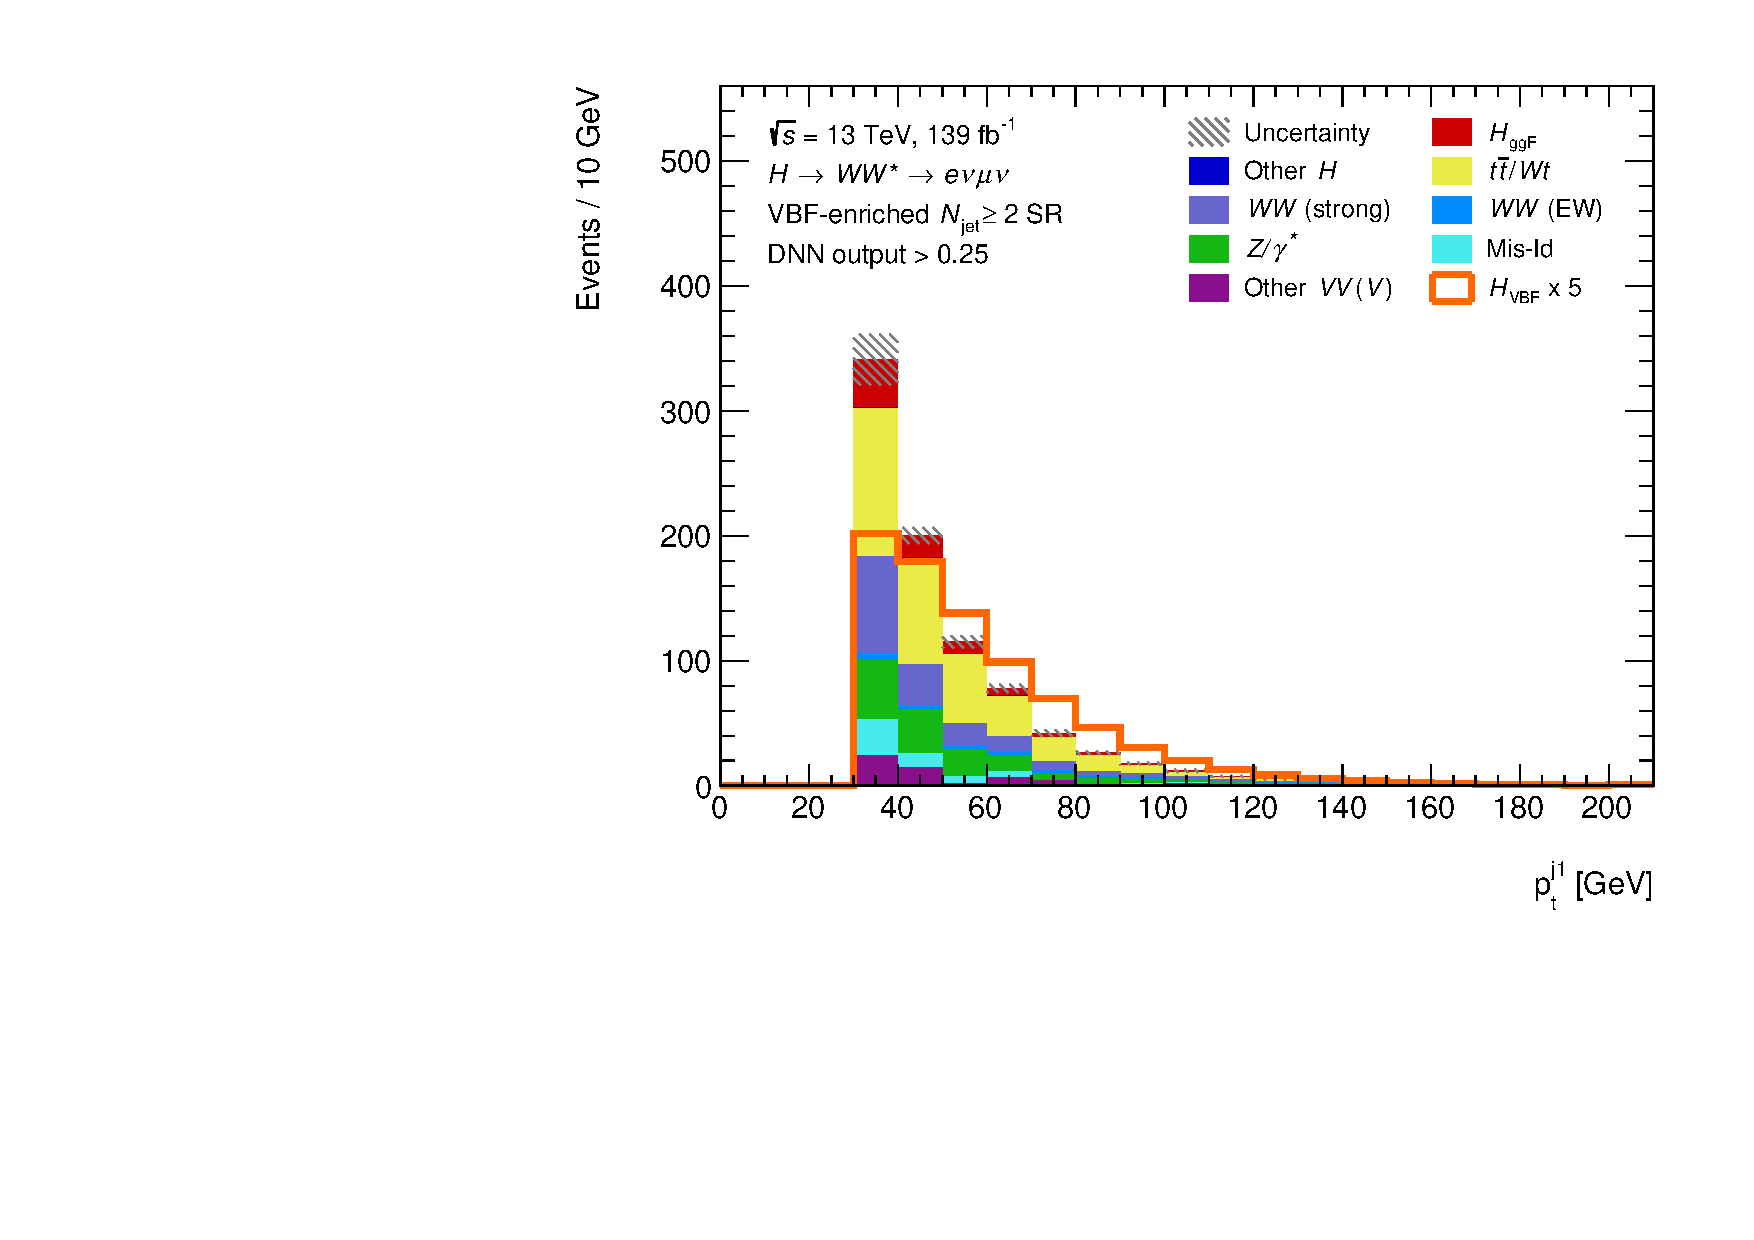
\includegraphics[width=0.32\textwidth]{figures/hww/dnn/blinded/run2-emme-CutVBFSR_DNN25-subleadJetPt-lin.pdf} \hfill
        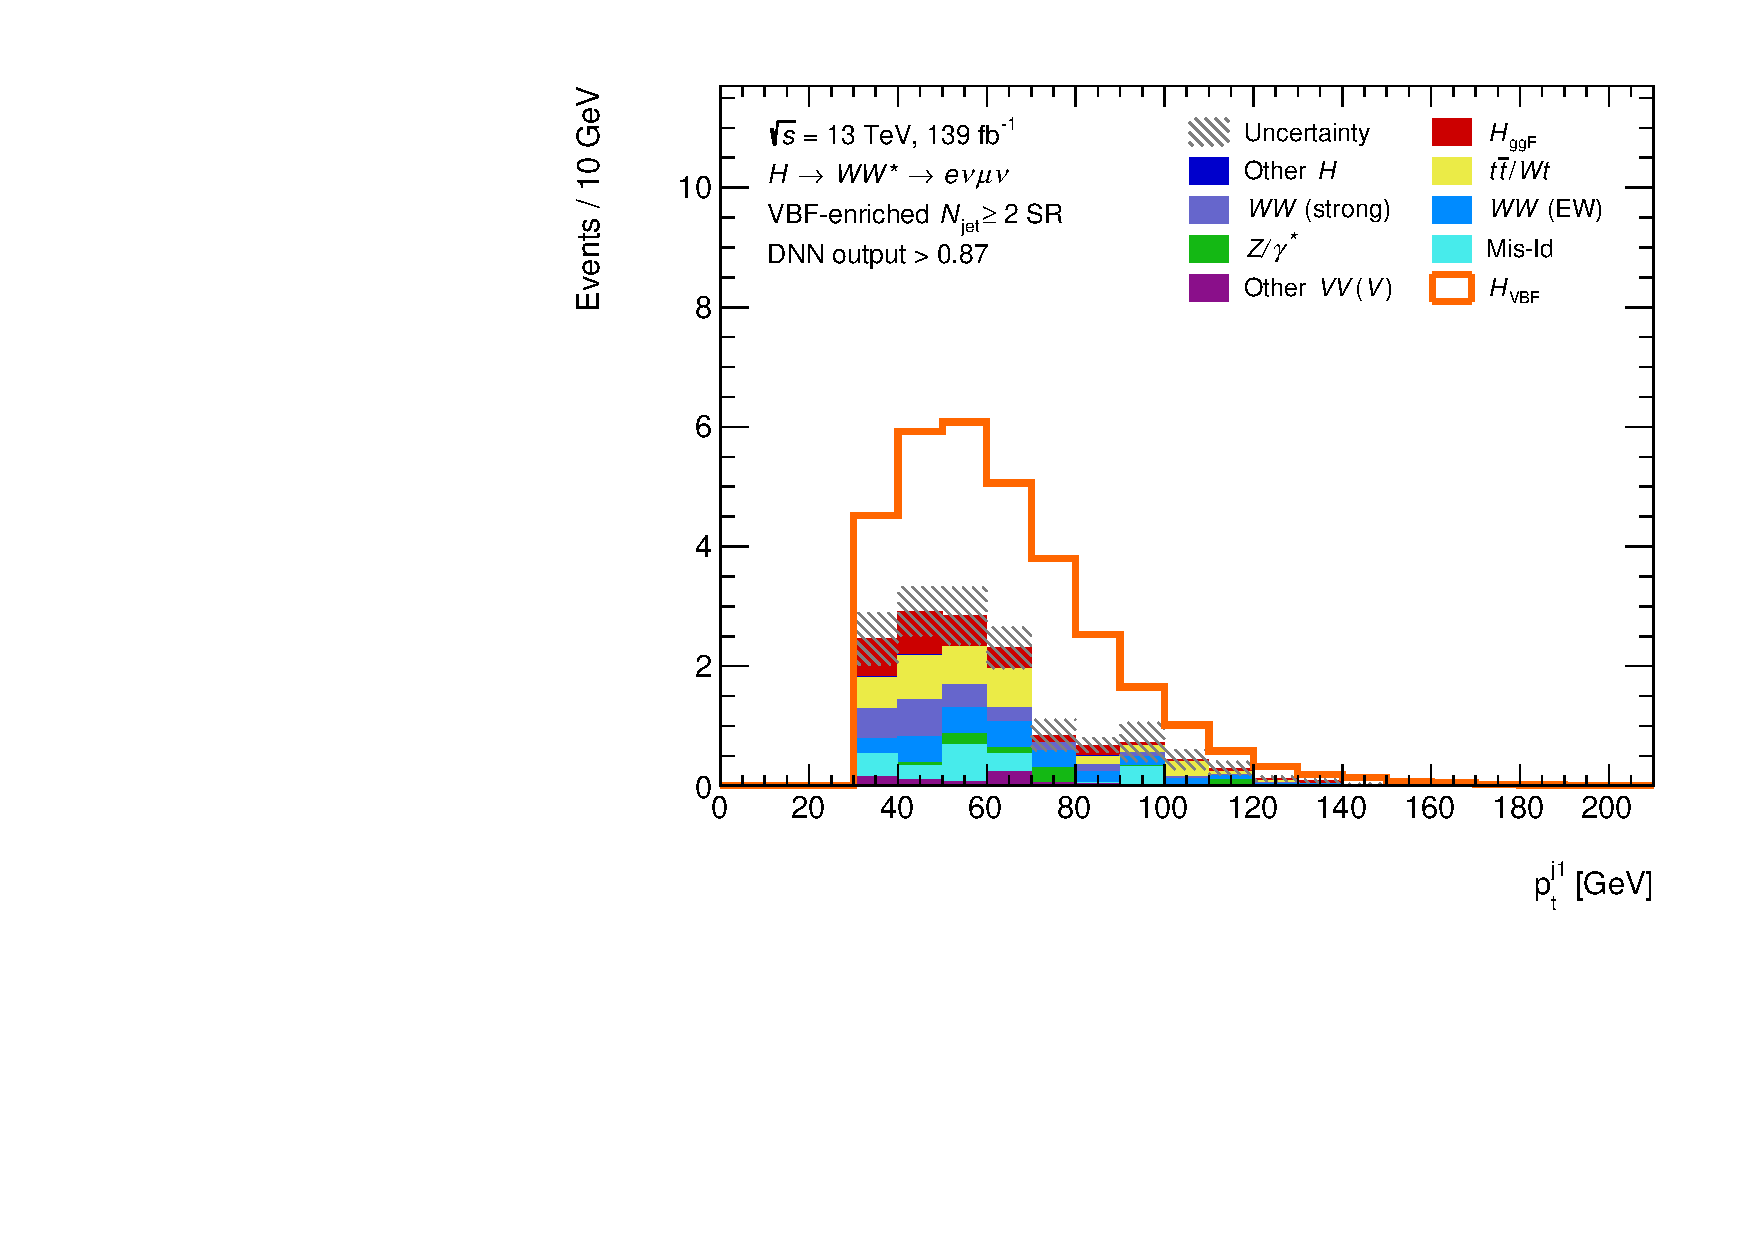
\includegraphics[width=0.32\textwidth]{figures/hww/dnn/blinded/run2-emme-CutVBFSR_DNN87-subleadJetPt-lin.pdf}
    } \\
    \subfloat[$\pTjthree$]{
        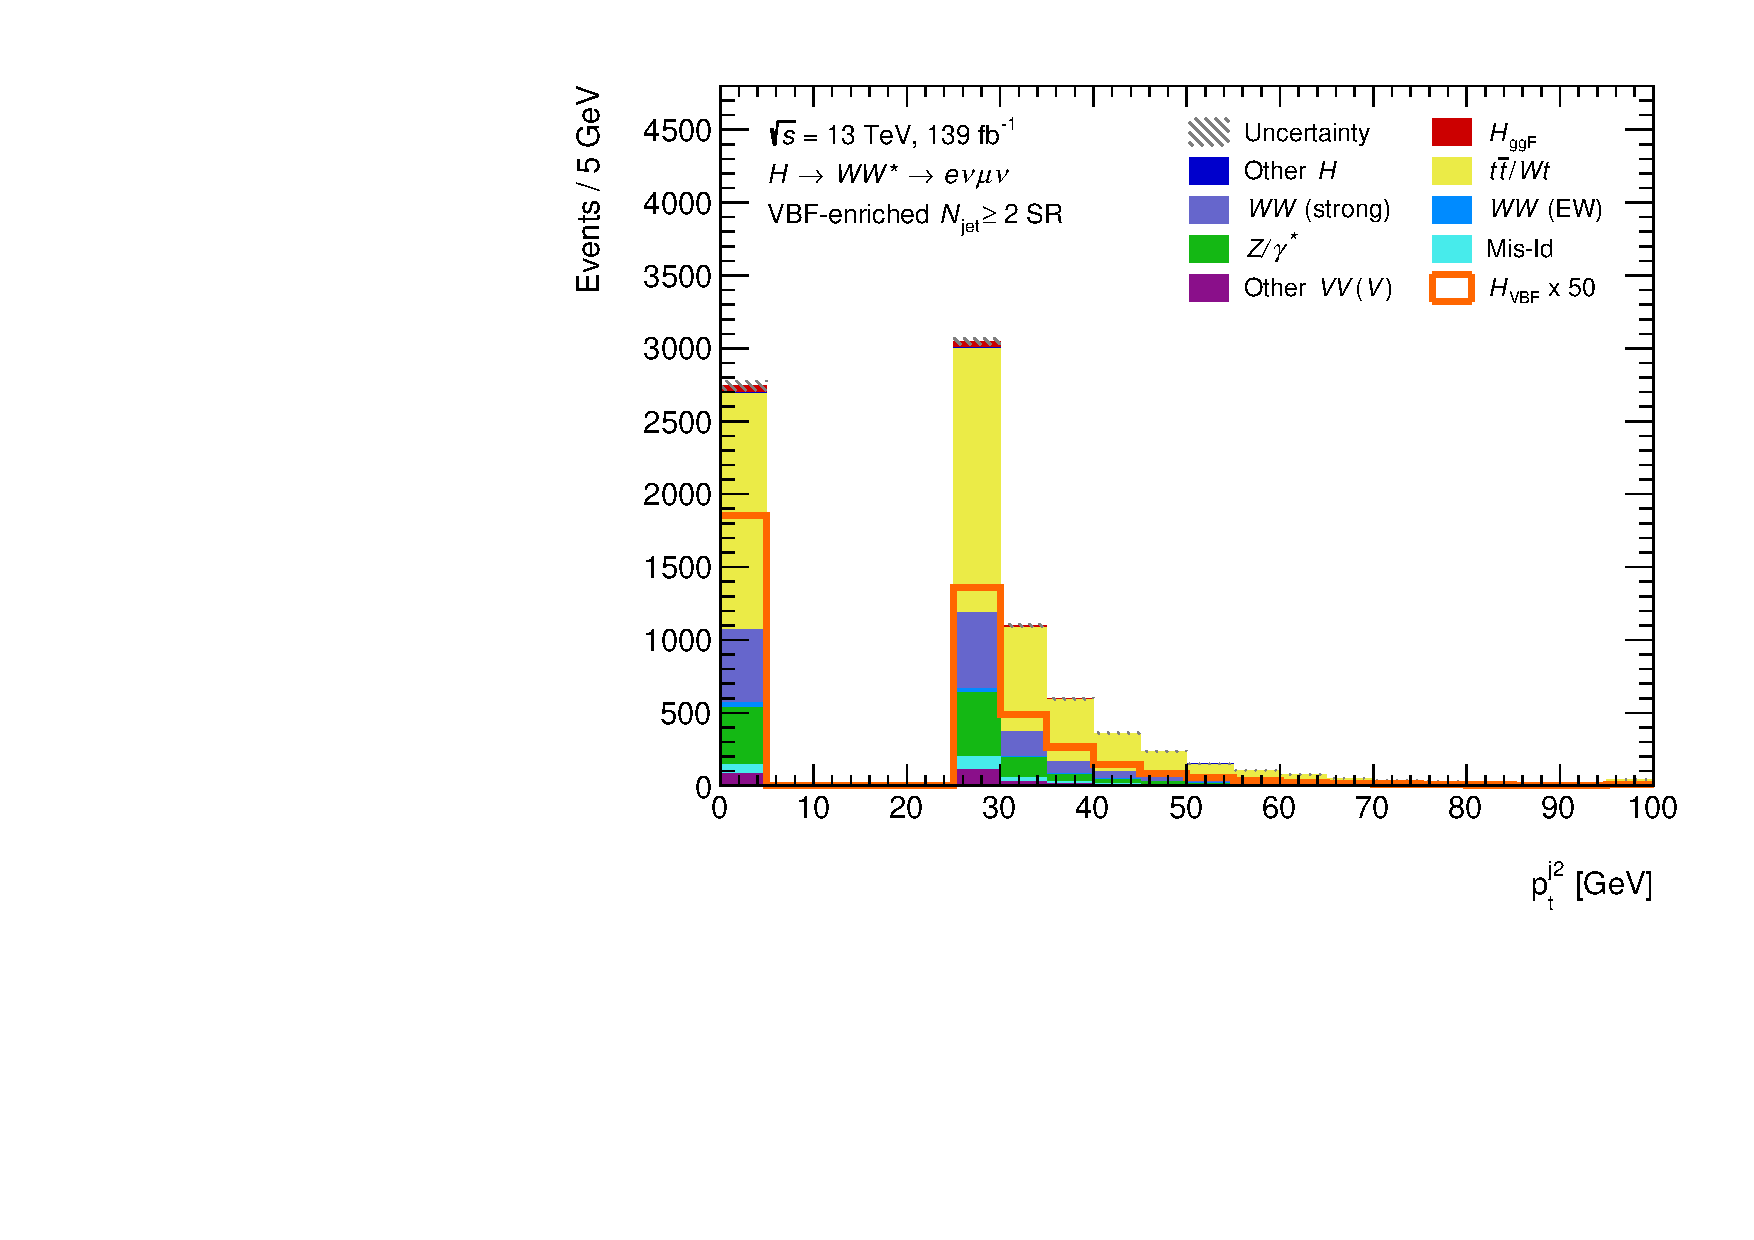
\includegraphics[width=0.32\textwidth]{figures/hww/dnn/blinded/run2-emme-CutVBF_SR-thirdJetPt-lin.pdf} \hfill
        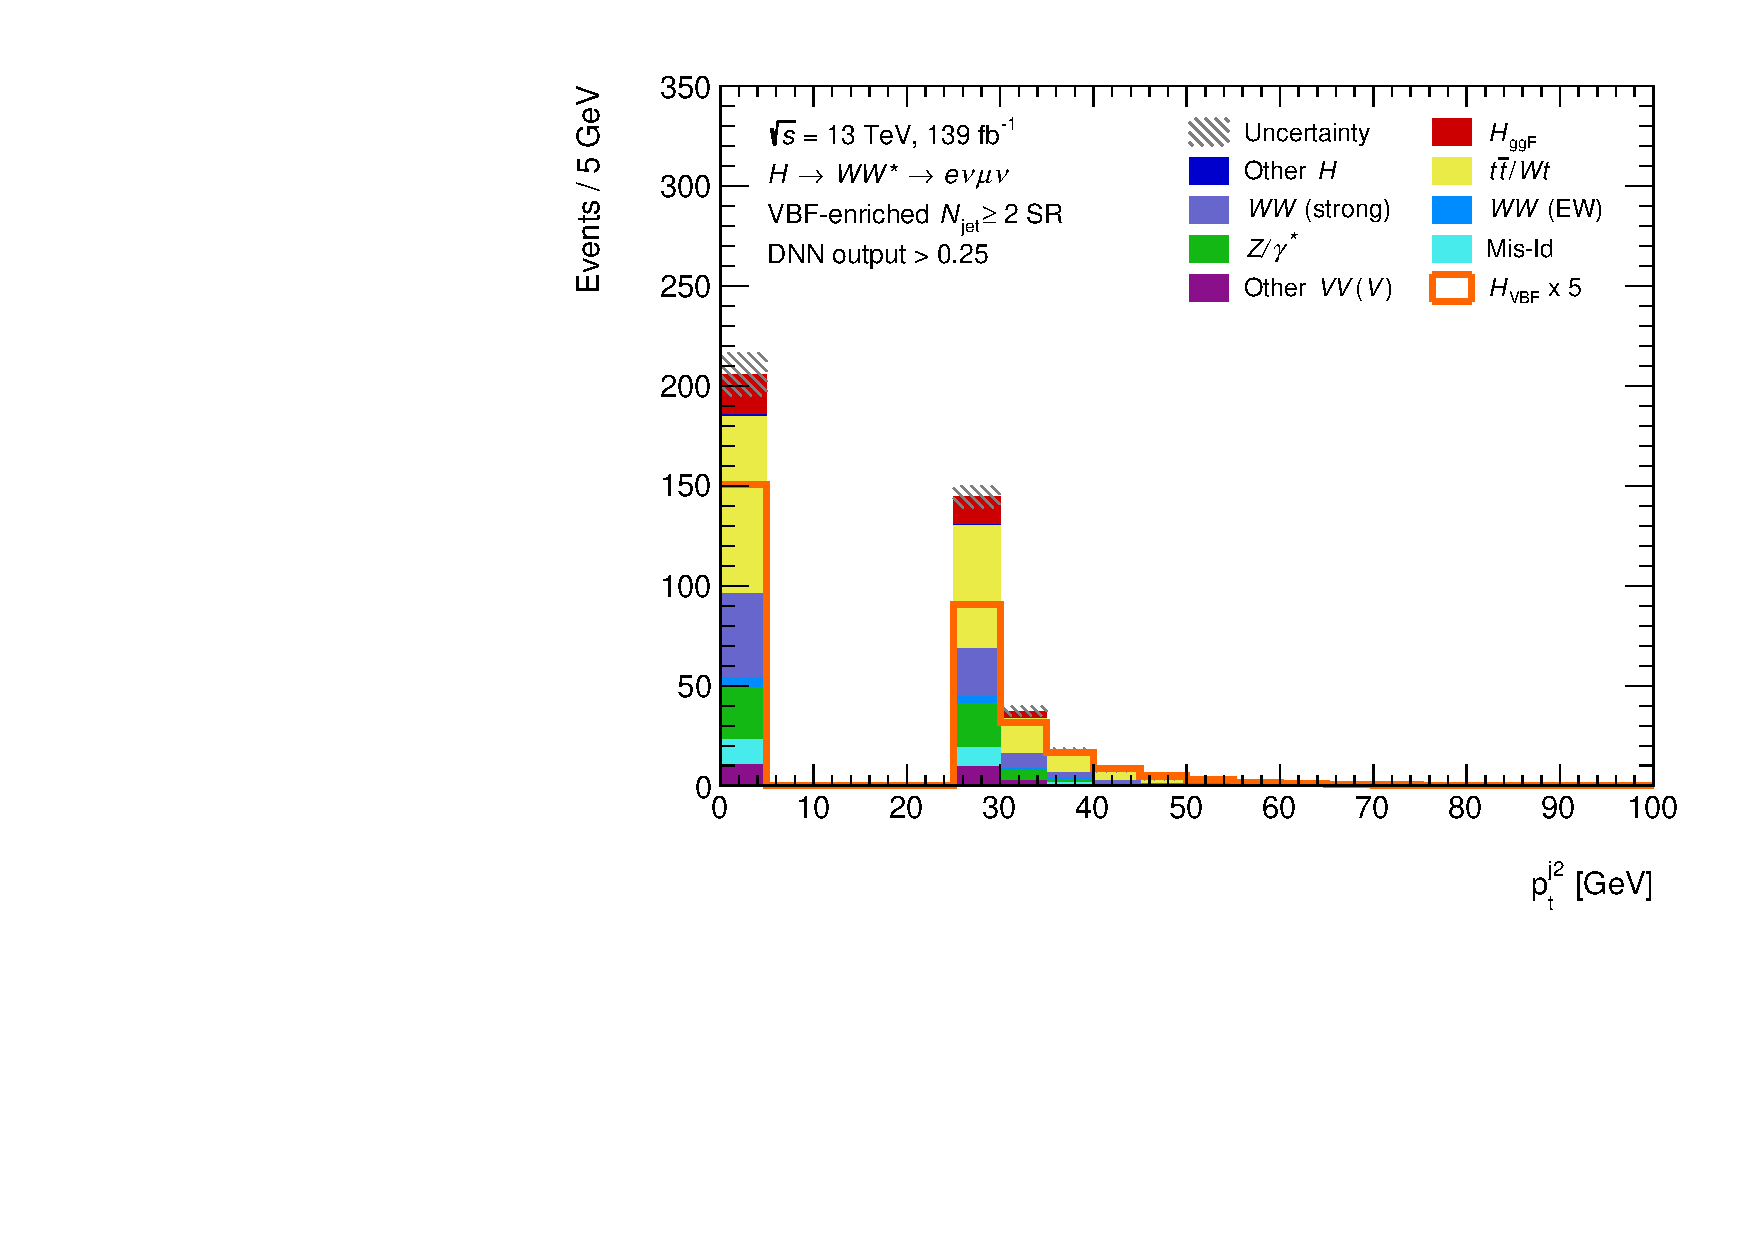
\includegraphics[width=0.32\textwidth]{figures/hww/dnn/blinded/run2-emme-CutVBFSR_DNN25-thirdJetPt-lin.pdf} \hfill
        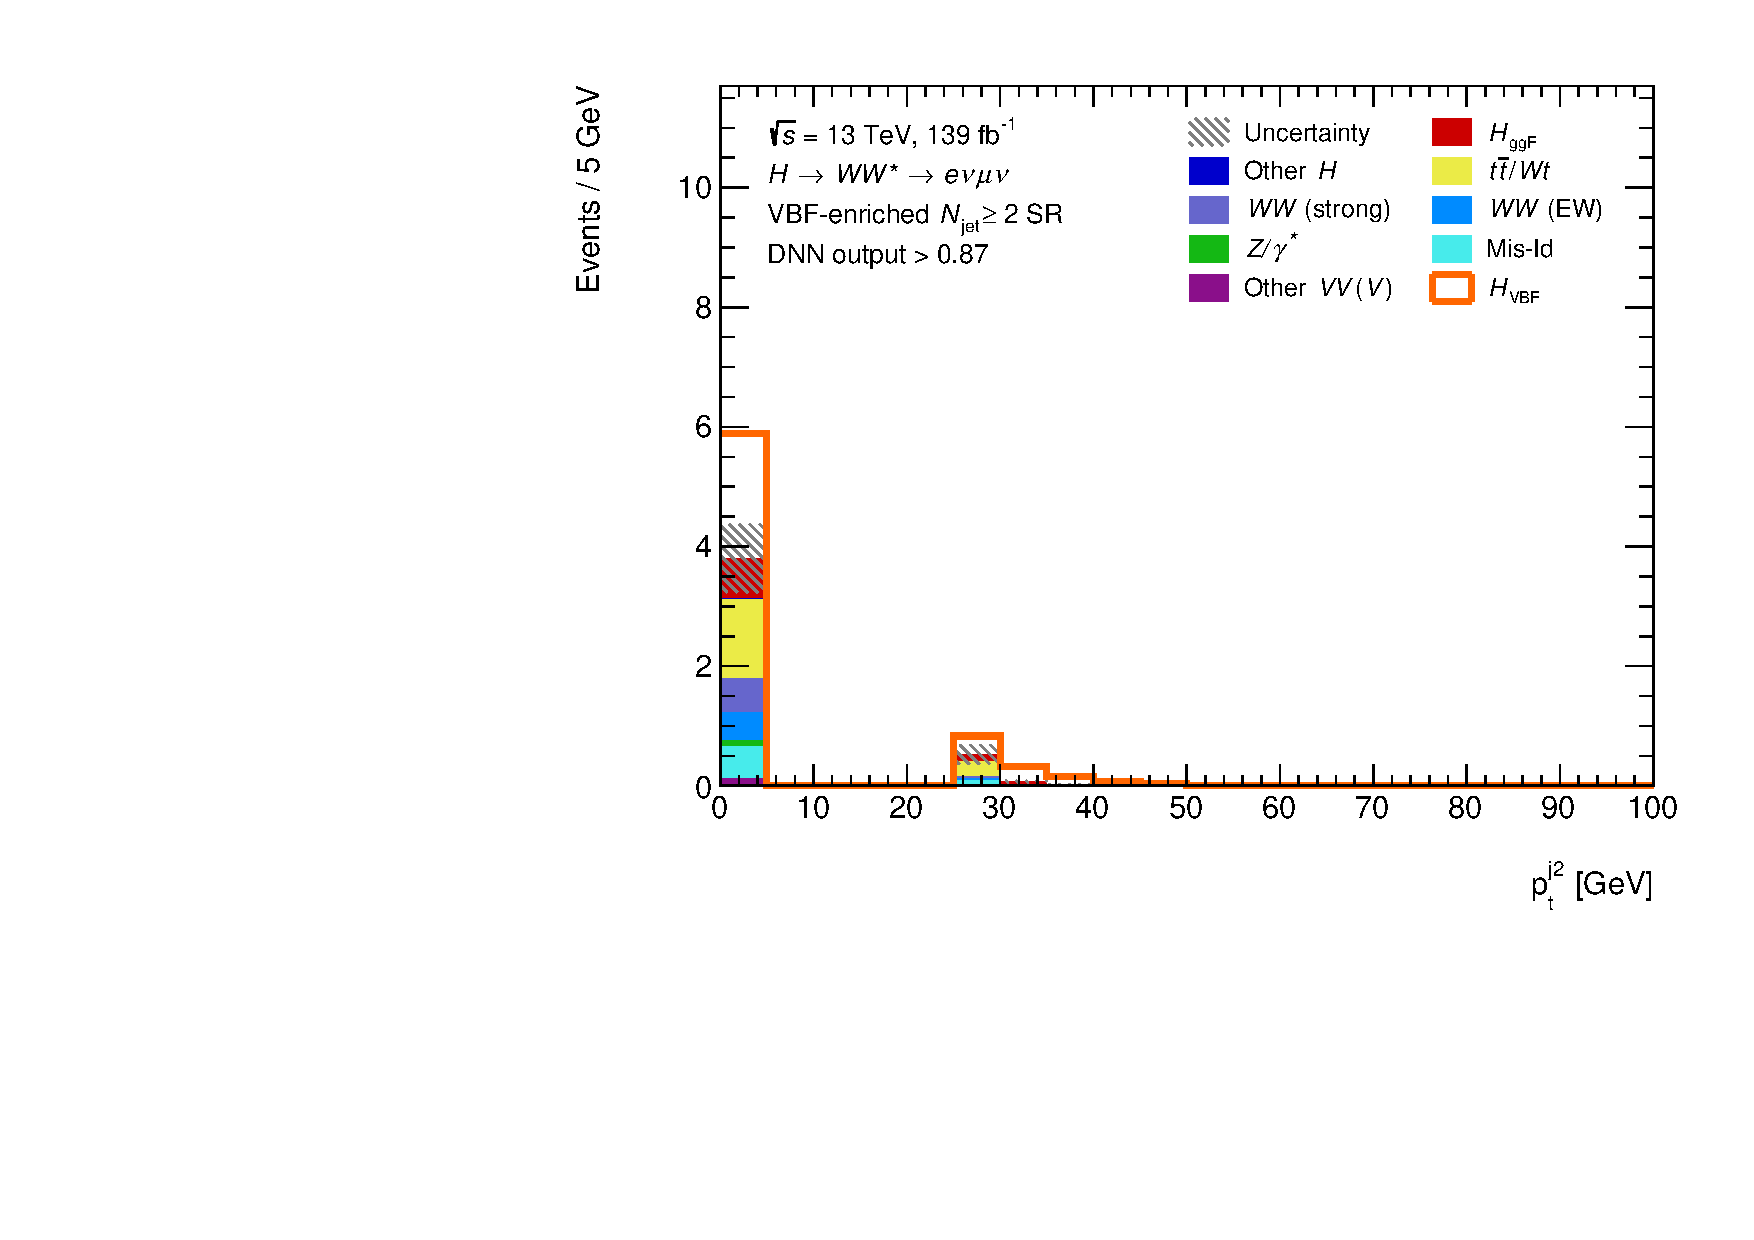
\includegraphics[width=0.32\textwidth]{figures/hww/dnn/blinded/run2-emme-CutVBFSR_DNN87-thirdJetPt-lin.pdf}
    } 
    {\caption{Distributions of $\pTjone$, $\pTjtwo$, and $\pTjthree$ in the VBF signal region.
            Each row shows one variable with different cuts on the DNN output distribution being applied in different columns.
            \label{fig:vbf:blindedSR2} }}
\end{figure}


\begin{figure}[h]
    \centering
    \subfloat[$\mlonejtwo$]{
        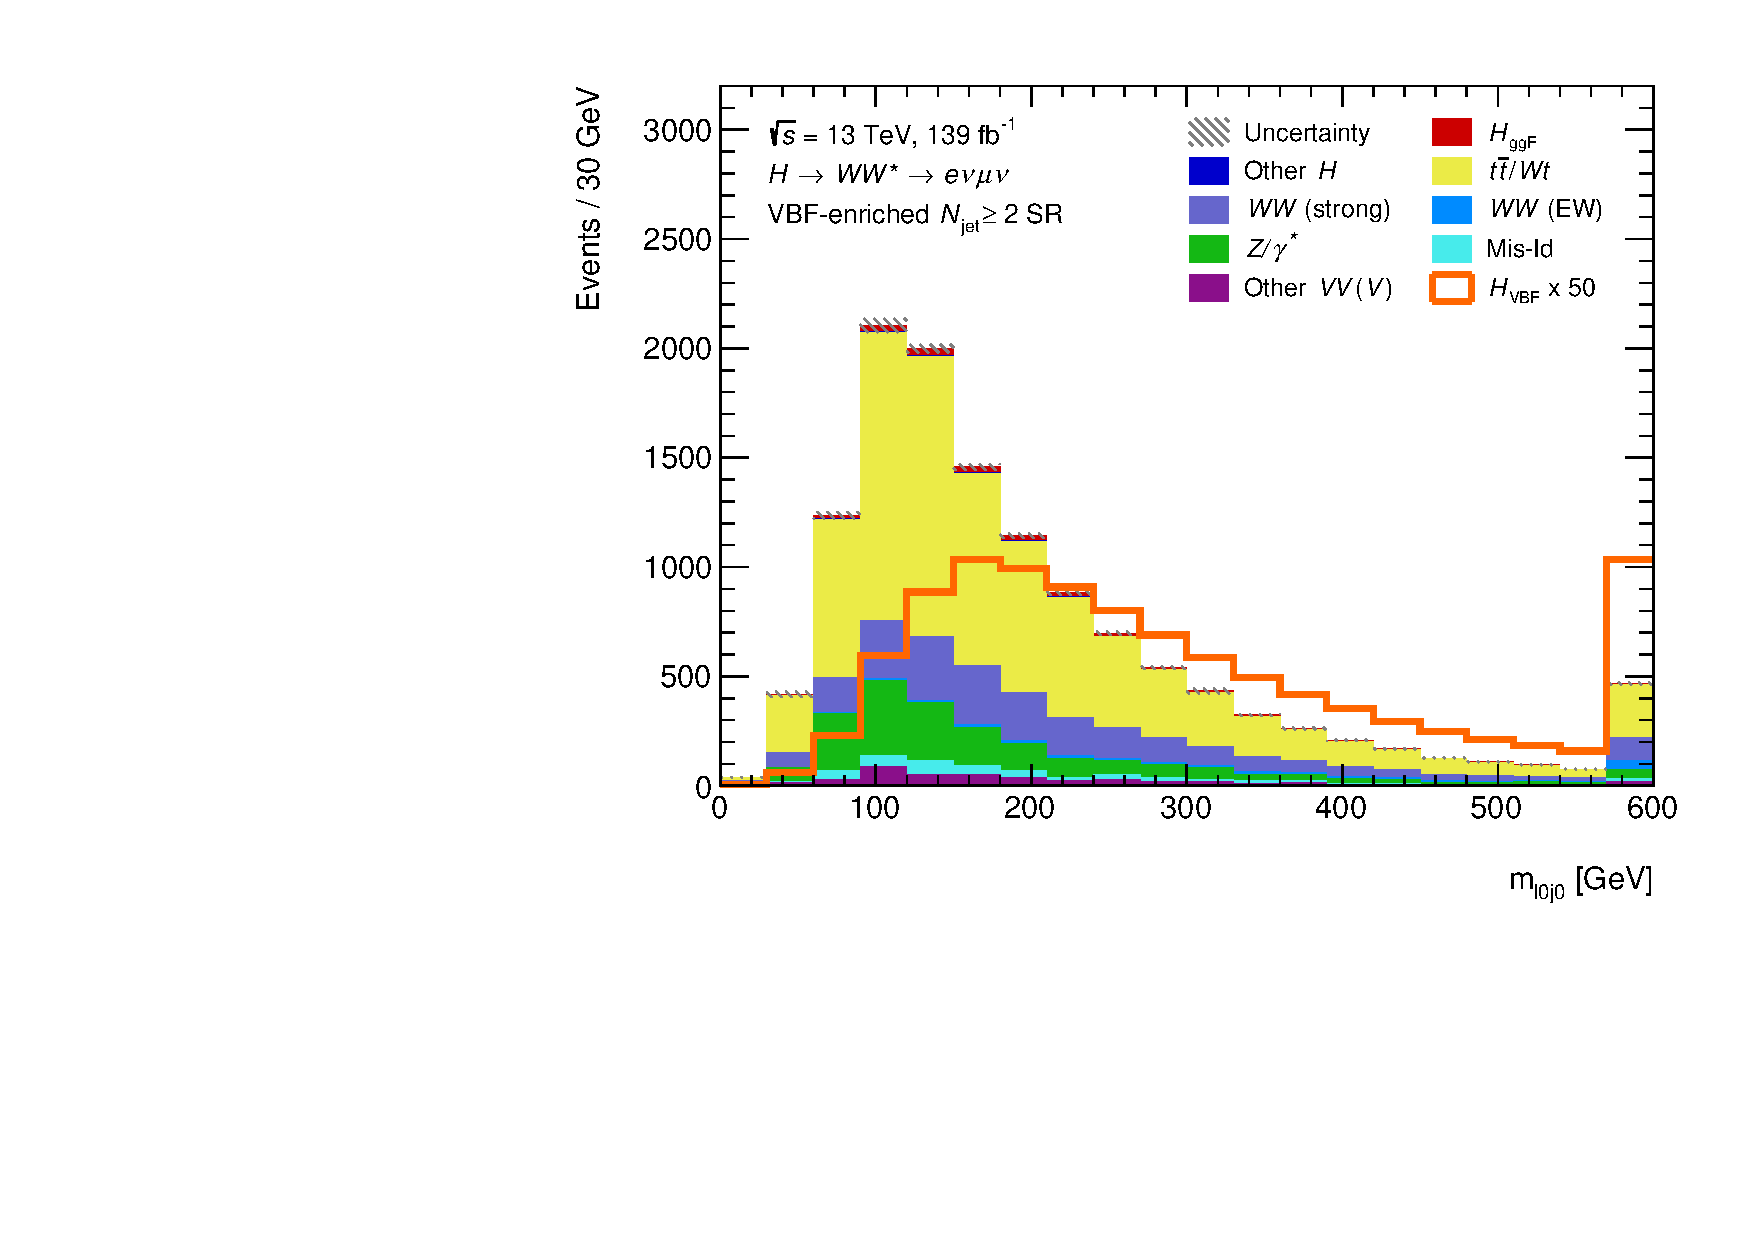
\includegraphics[width=0.32\textwidth]{figures/hww/dnn/blinded/run2-emme-CutVBF_SR-Ml0j0-lin.pdf} \hfill
        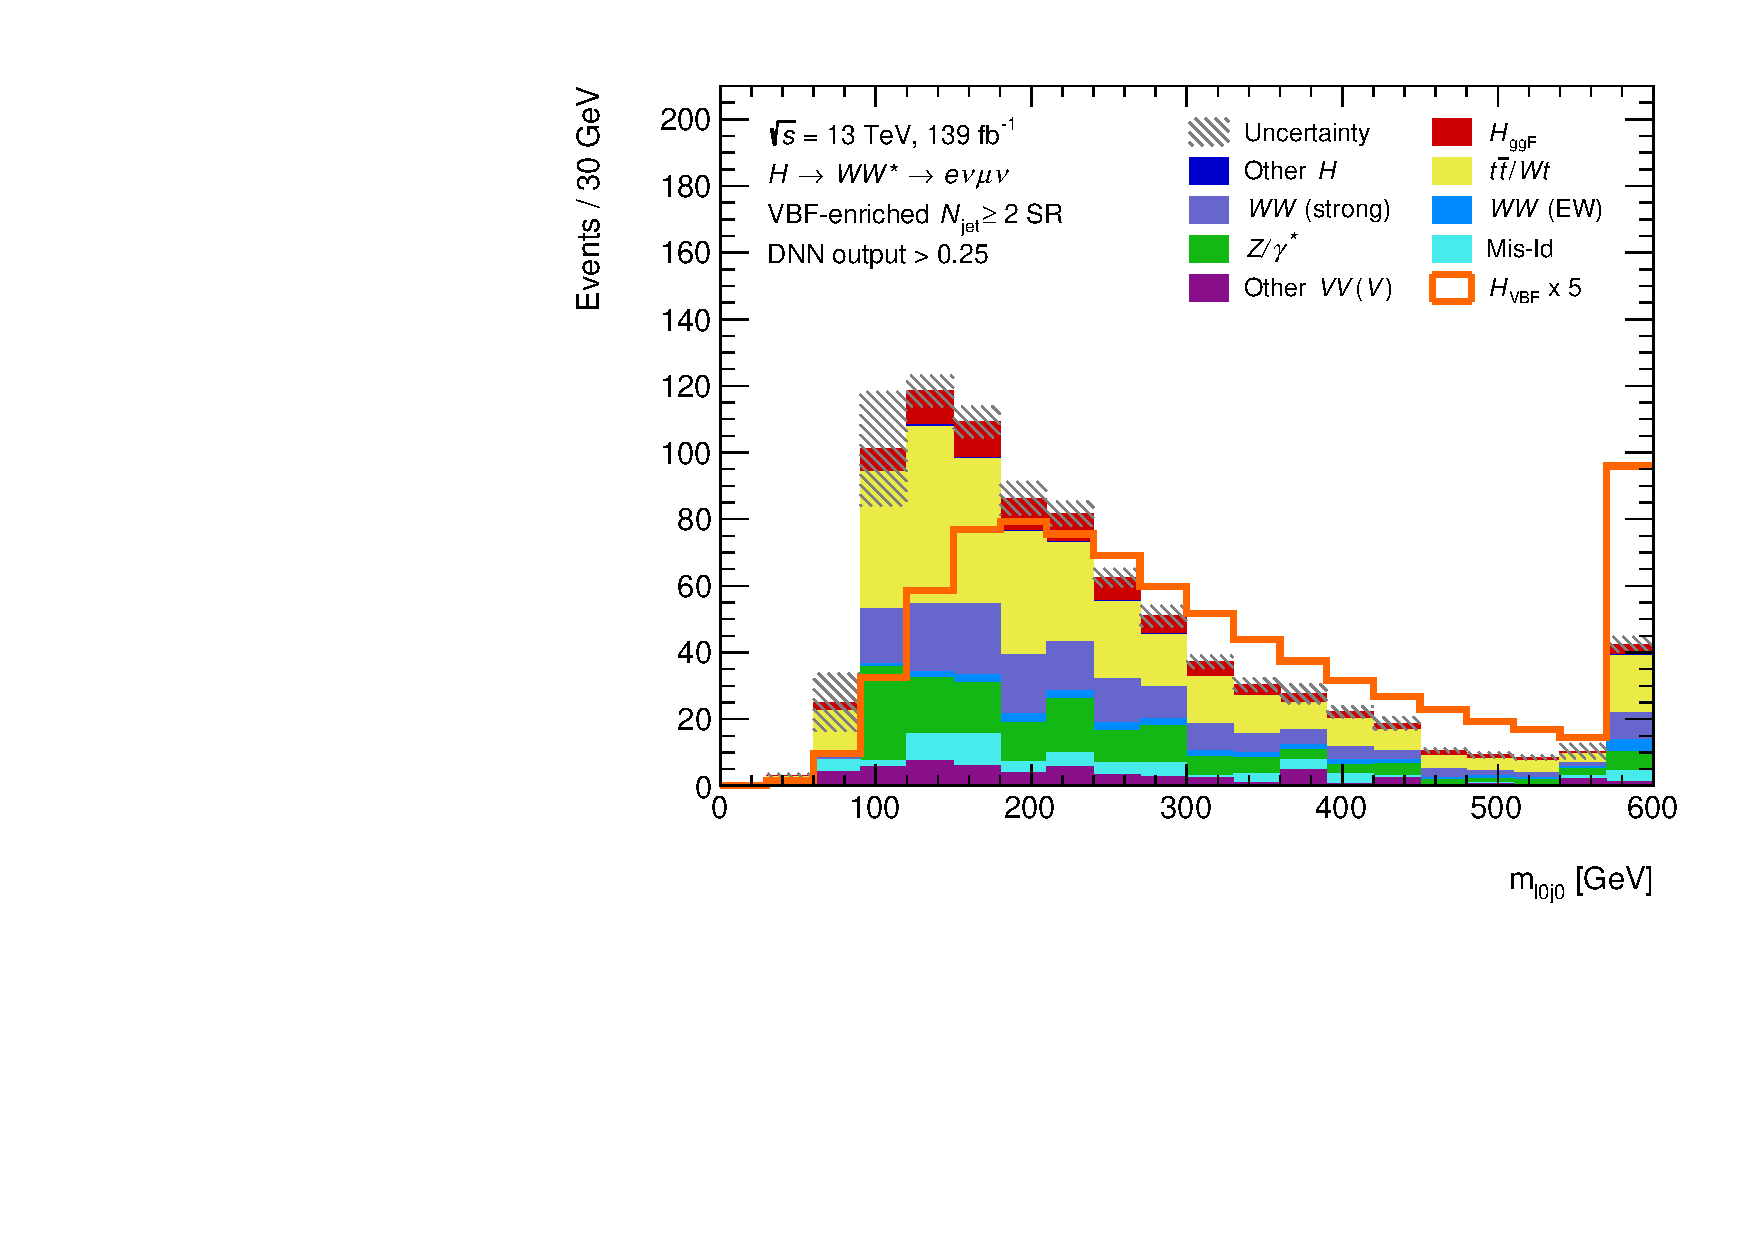
\includegraphics[width=0.32\textwidth]{figures/hww/dnn/blinded/run2-emme-CutVBFSR_DNN25-Ml0j0-lin.pdf} \hfill
        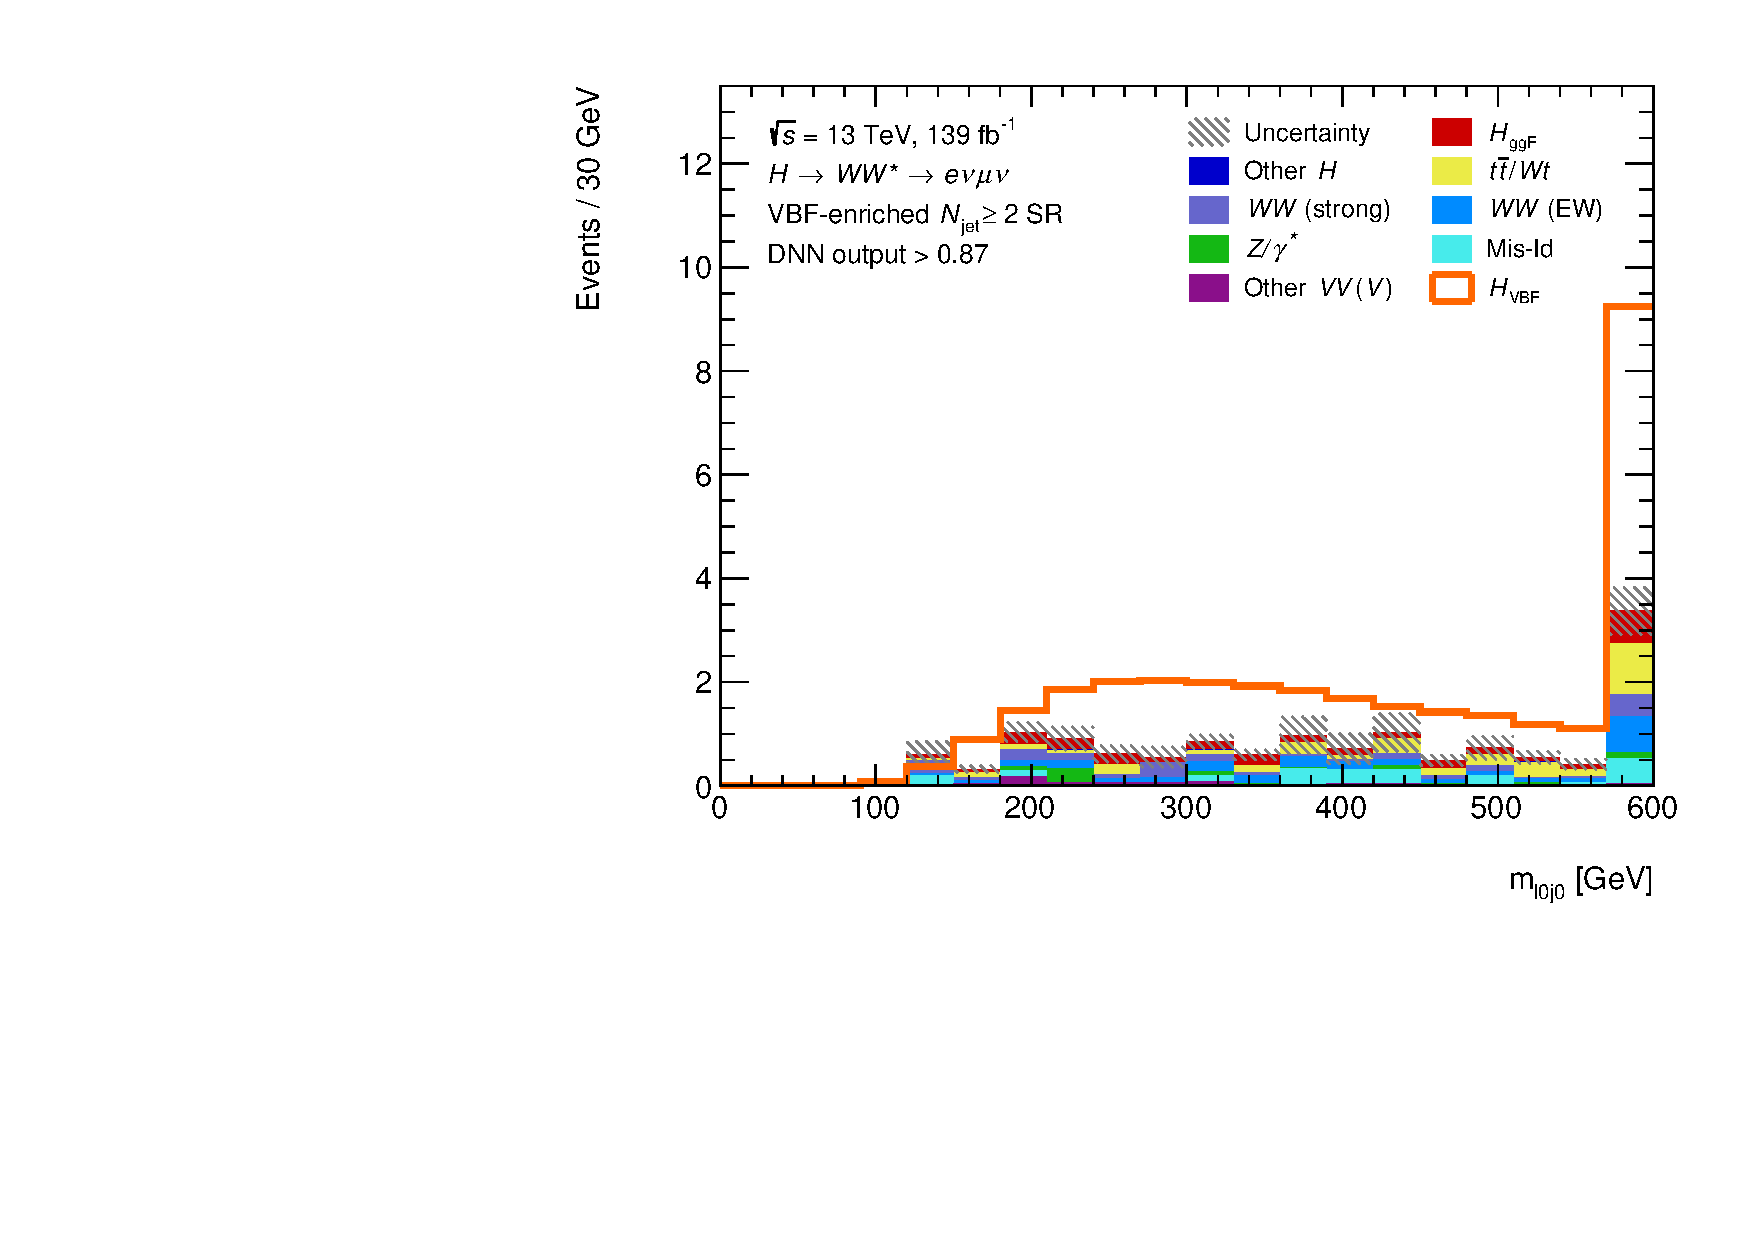
\includegraphics[width=0.32\textwidth]{figures/hww/dnn/blinded/run2-emme-CutVBFSR_DNN87-Ml0j0-lin.pdf}
    } \\
    \subfloat[$\mltwojone$]{
        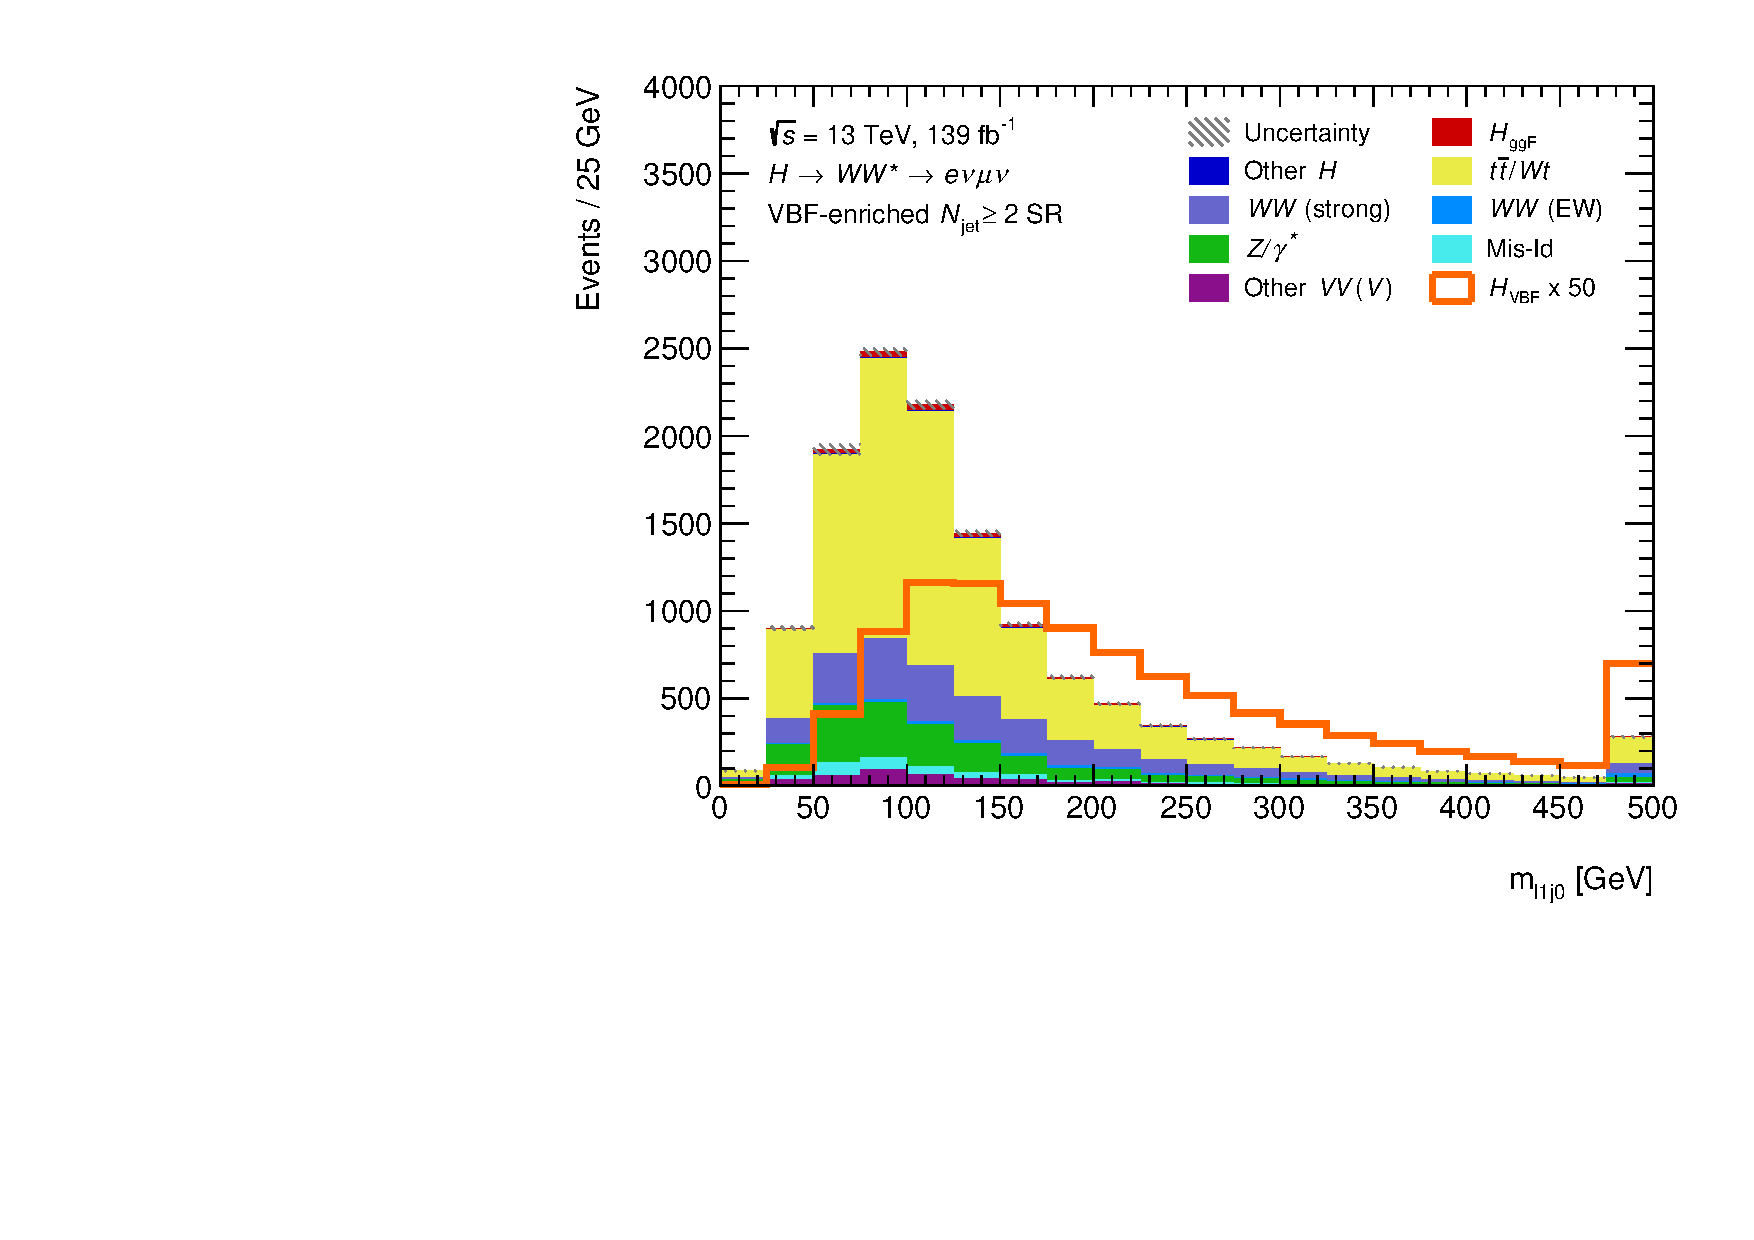
\includegraphics[width=0.32\textwidth]{figures/hww/dnn/blinded/run2-emme-CutVBF_SR-Ml1j0-lin.pdf} \hfill
        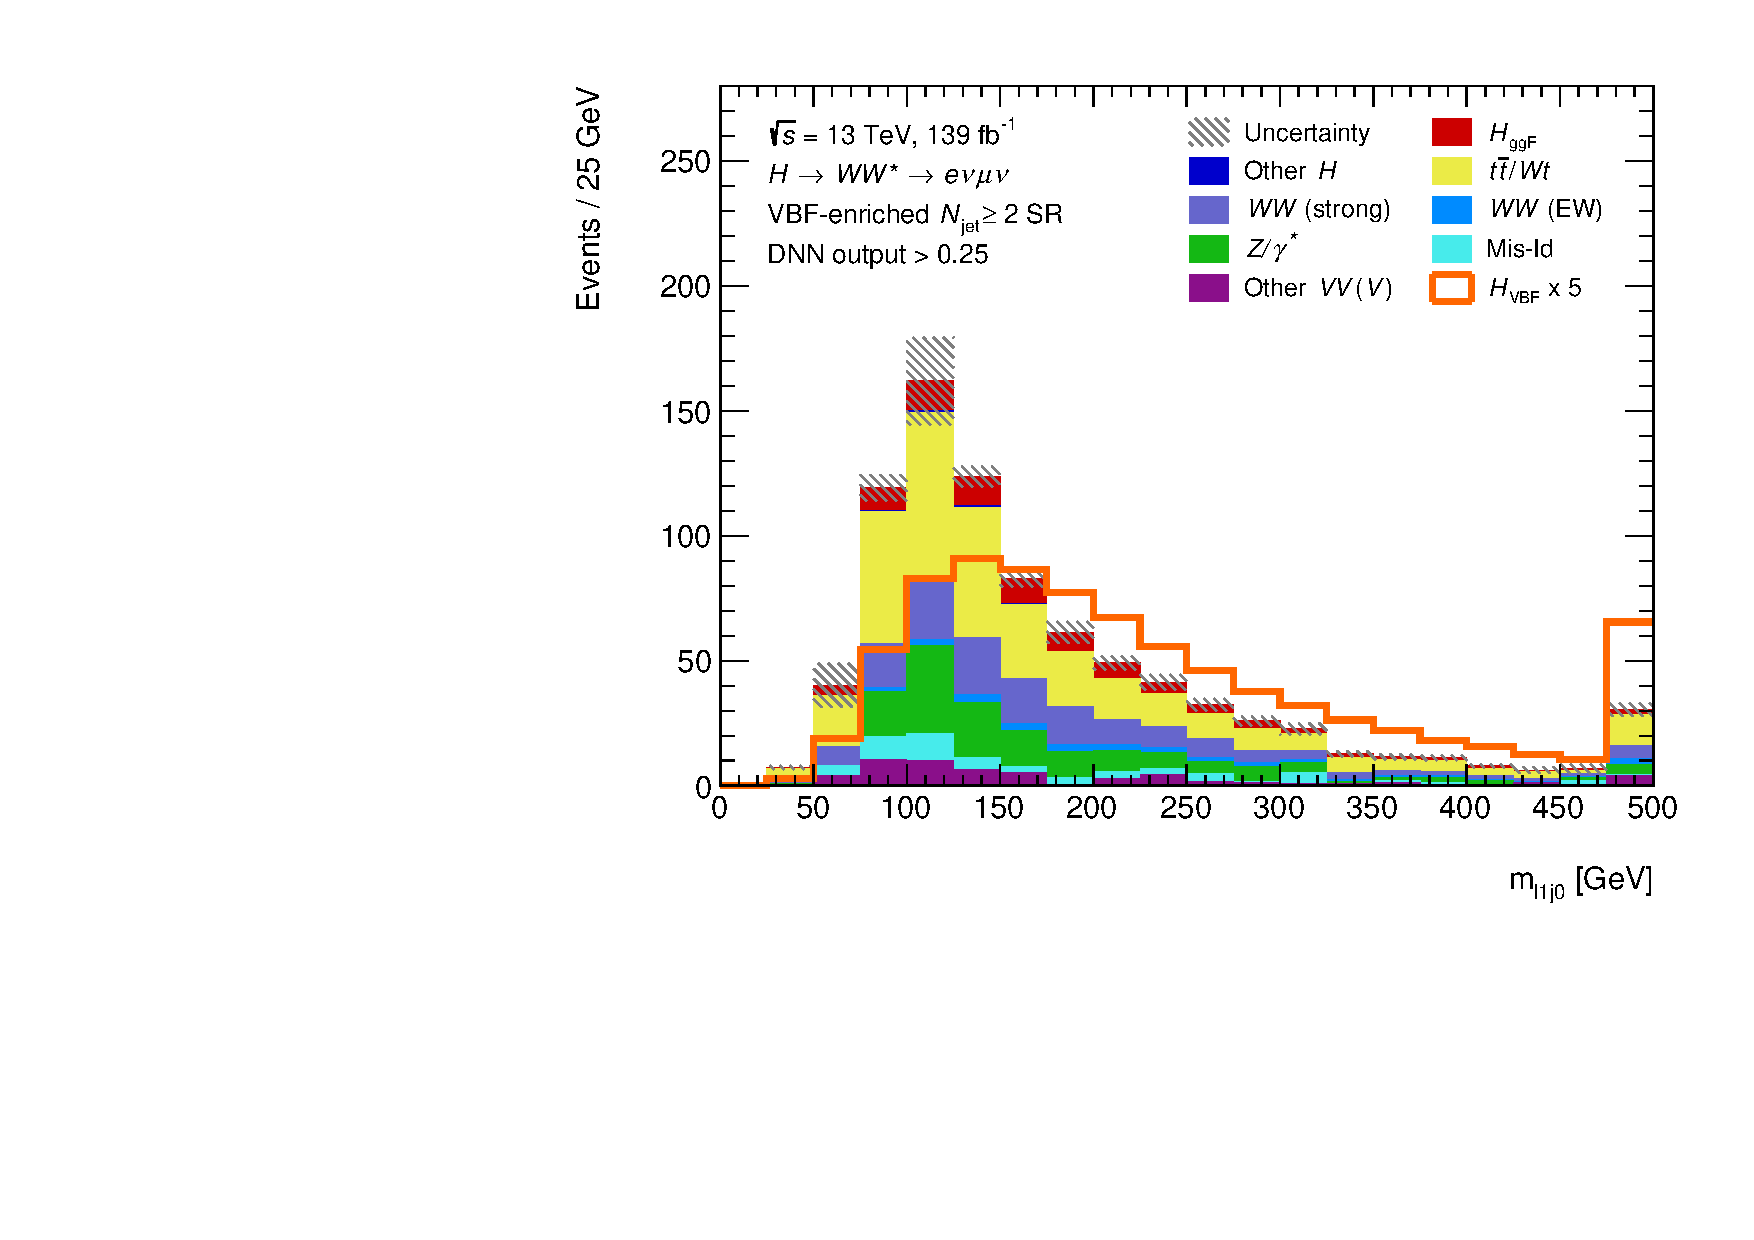
\includegraphics[width=0.32\textwidth]{figures/hww/dnn/blinded/run2-emme-CutVBFSR_DNN25-Ml1j0-lin.pdf} \hfill
        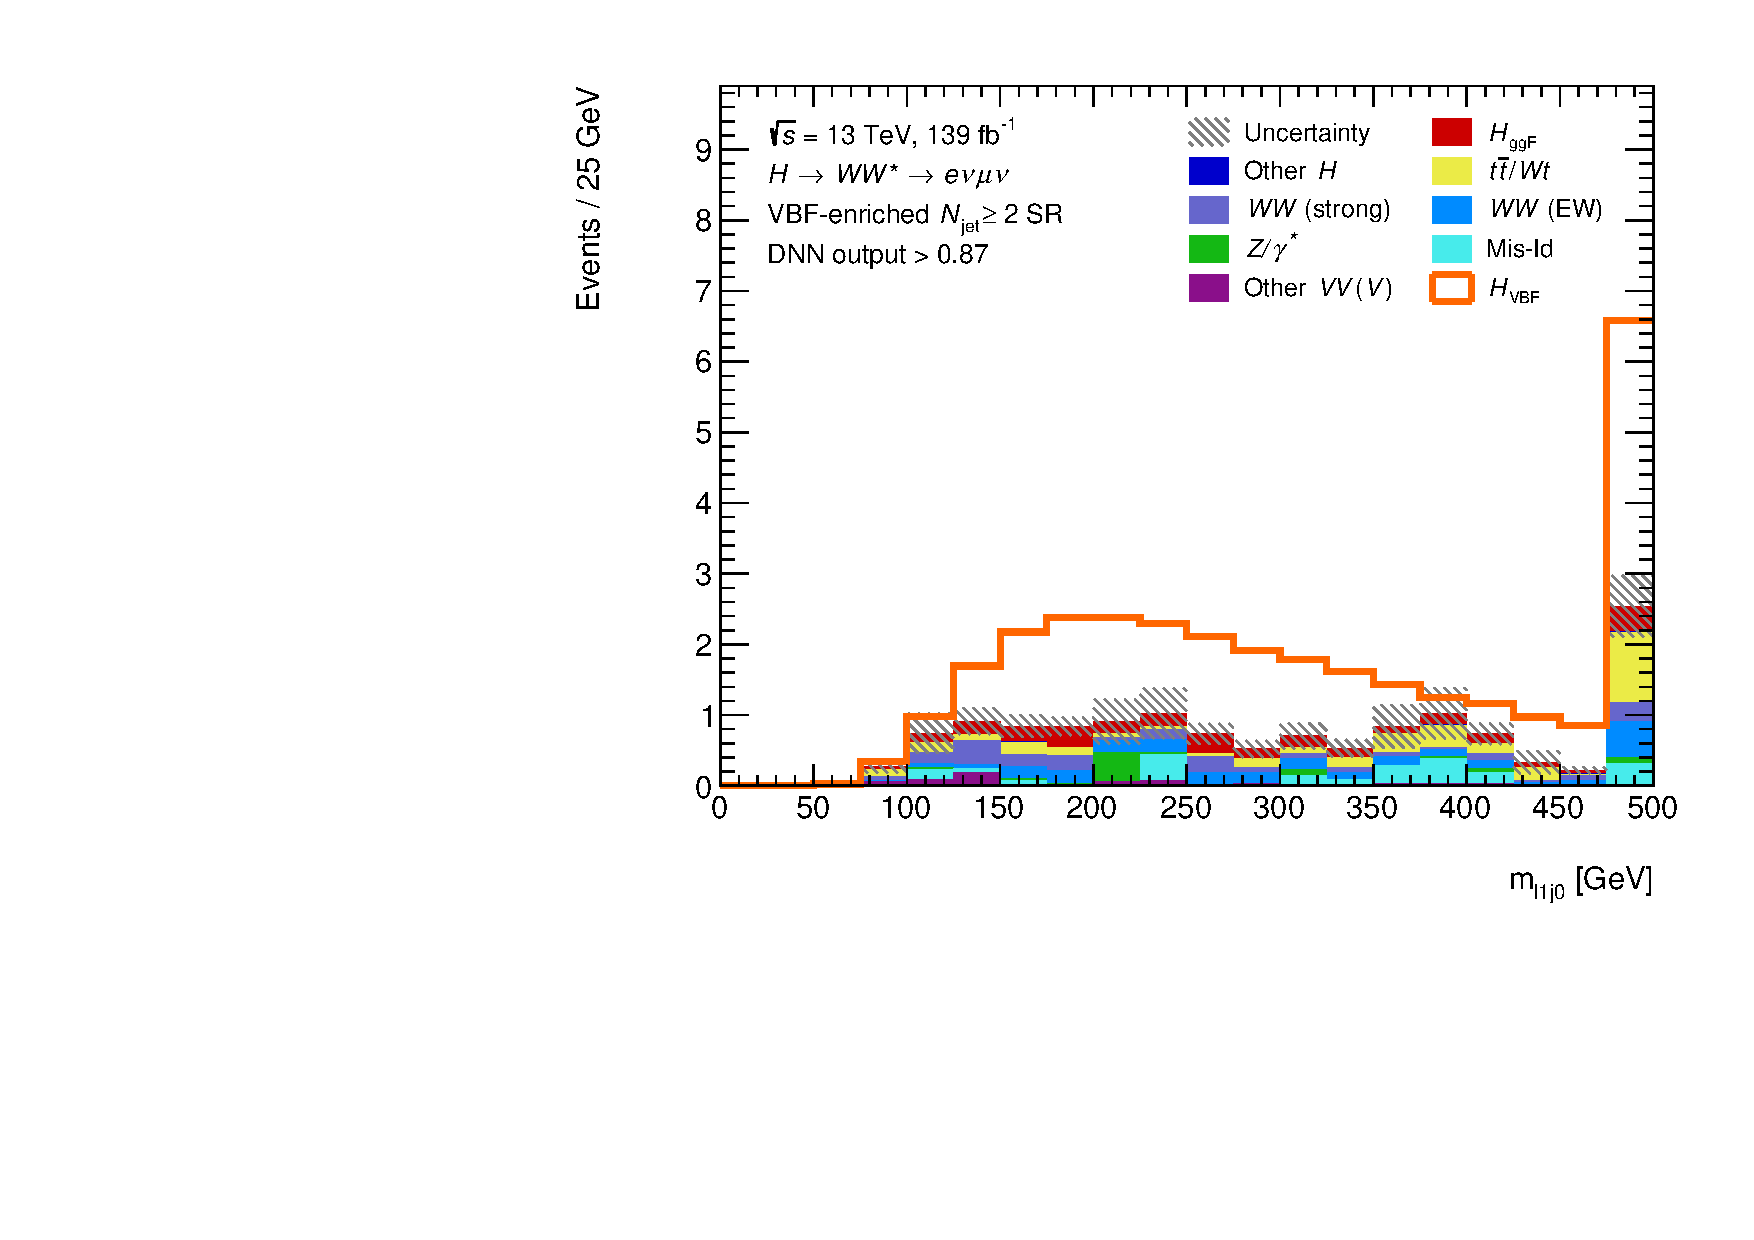
\includegraphics[width=0.32\textwidth]{figures/hww/dnn/blinded/run2-emme-CutVBFSR_DNN87-Ml1j0-lin.pdf}
    } \\
    \subfloat[$\mlonejtwo$]{
        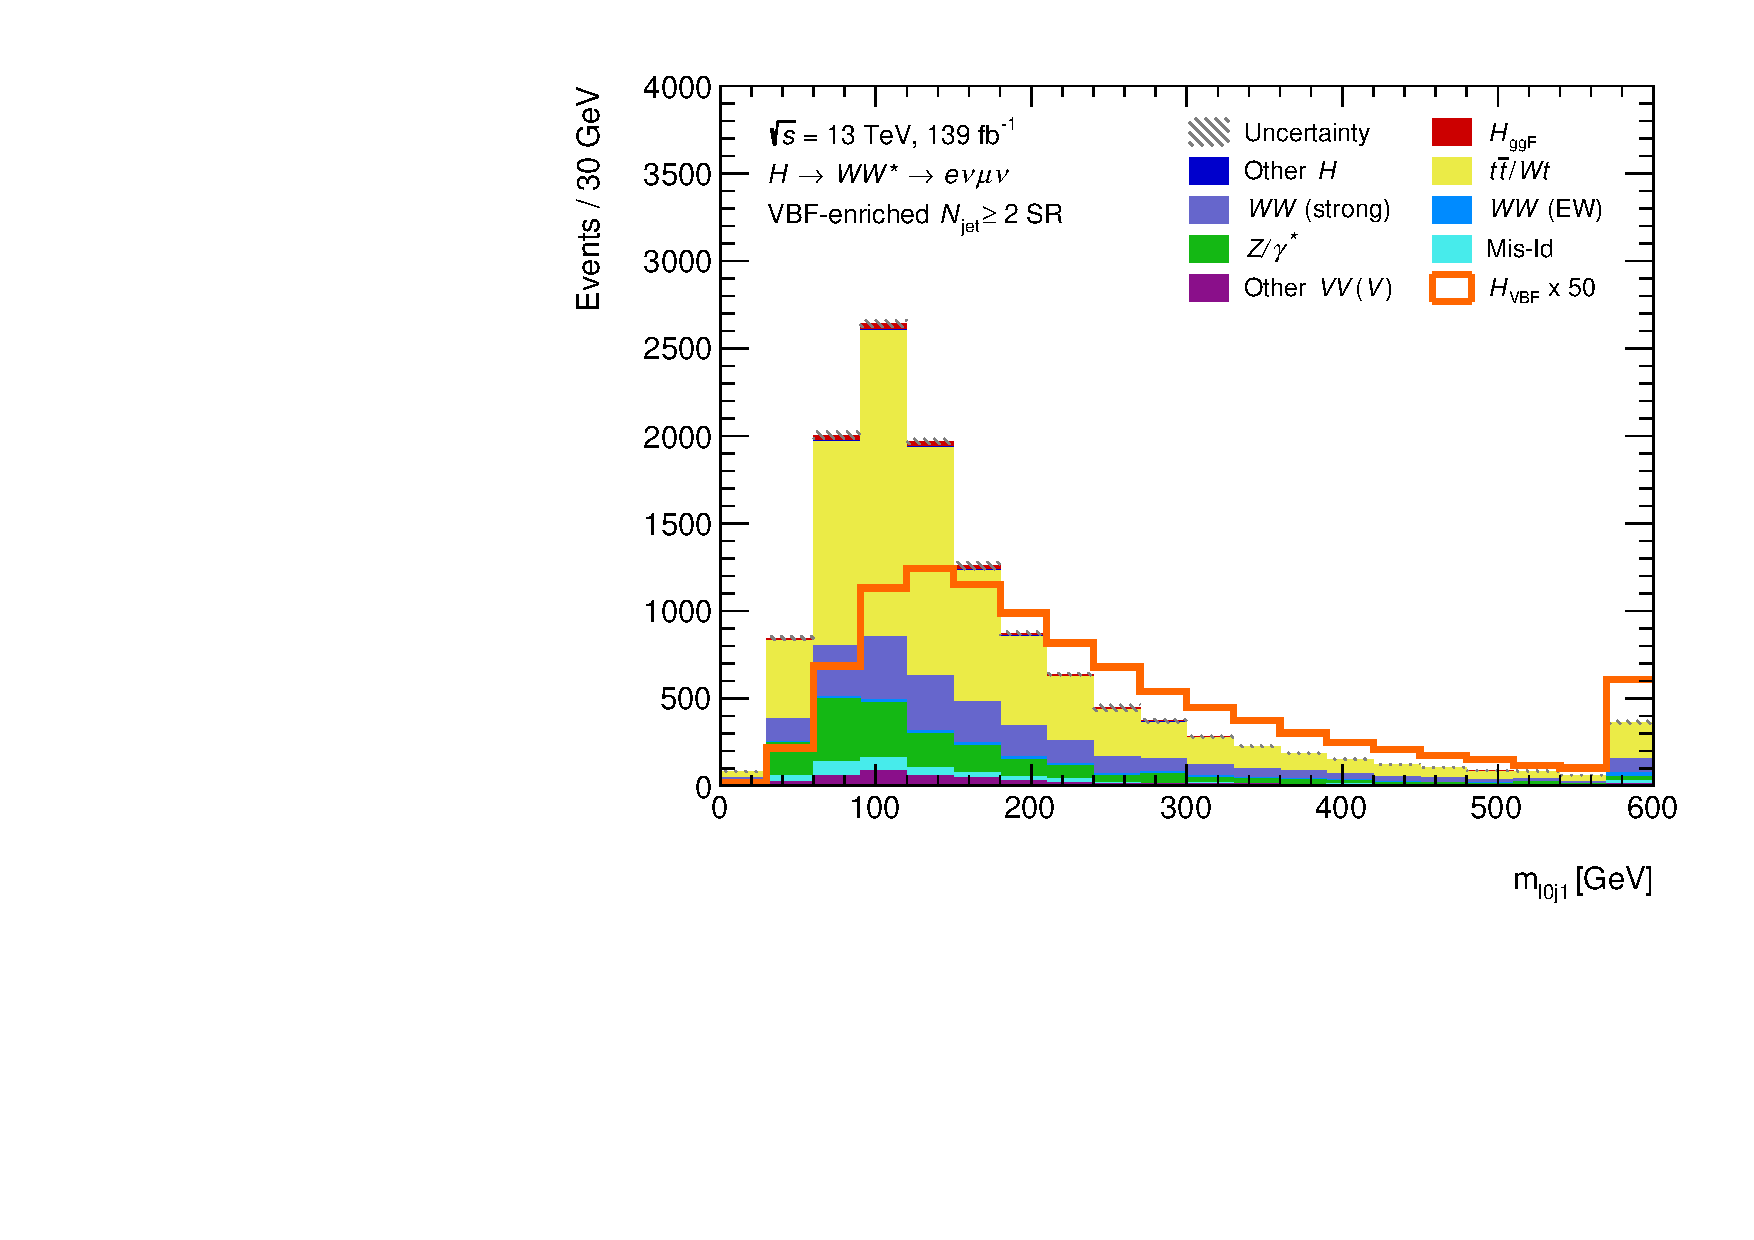
\includegraphics[width=0.32\textwidth]{figures/hww/dnn/blinded/run2-emme-CutVBF_SR-Ml0j1-lin.pdf} \hfill
        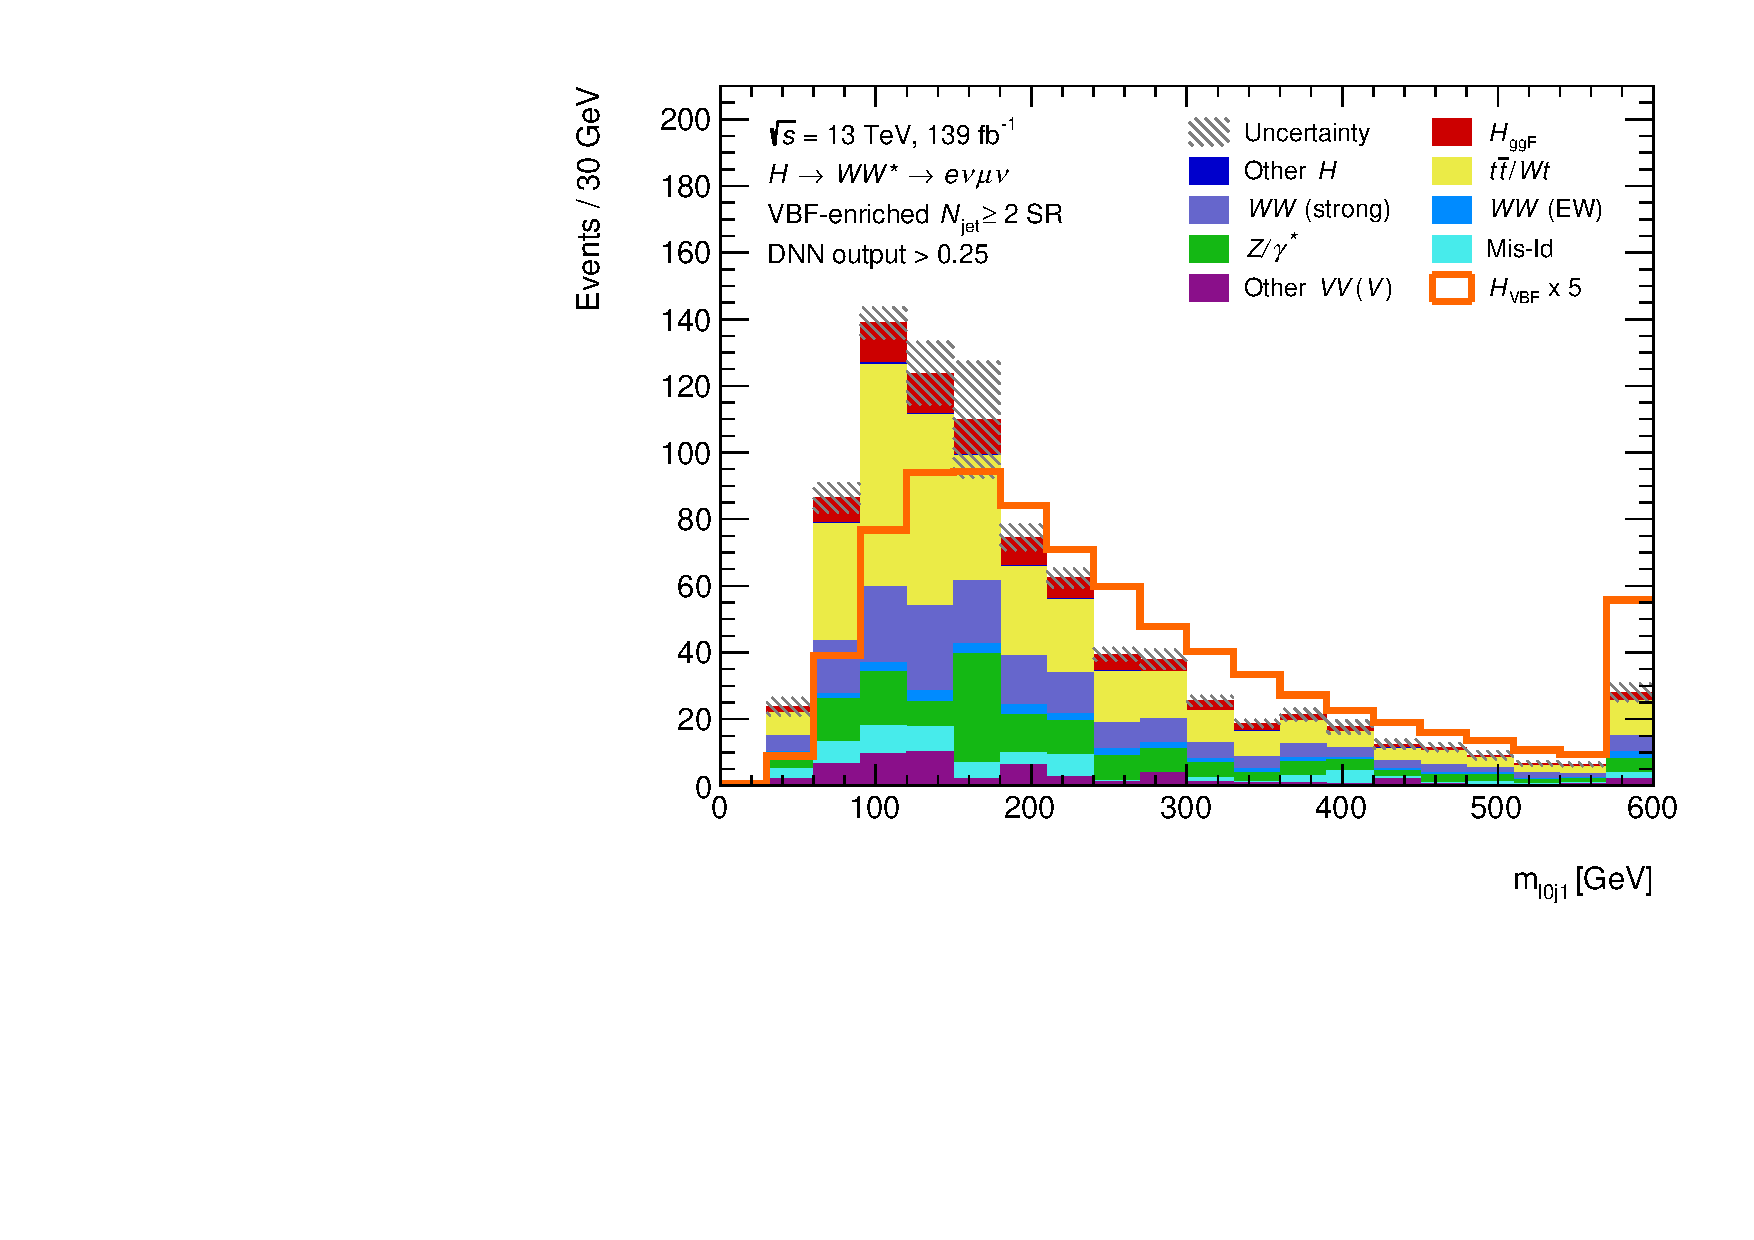
\includegraphics[width=0.32\textwidth]{figures/hww/dnn/blinded/run2-emme-CutVBFSR_DNN25-Ml0j1-lin.pdf} \hfill
        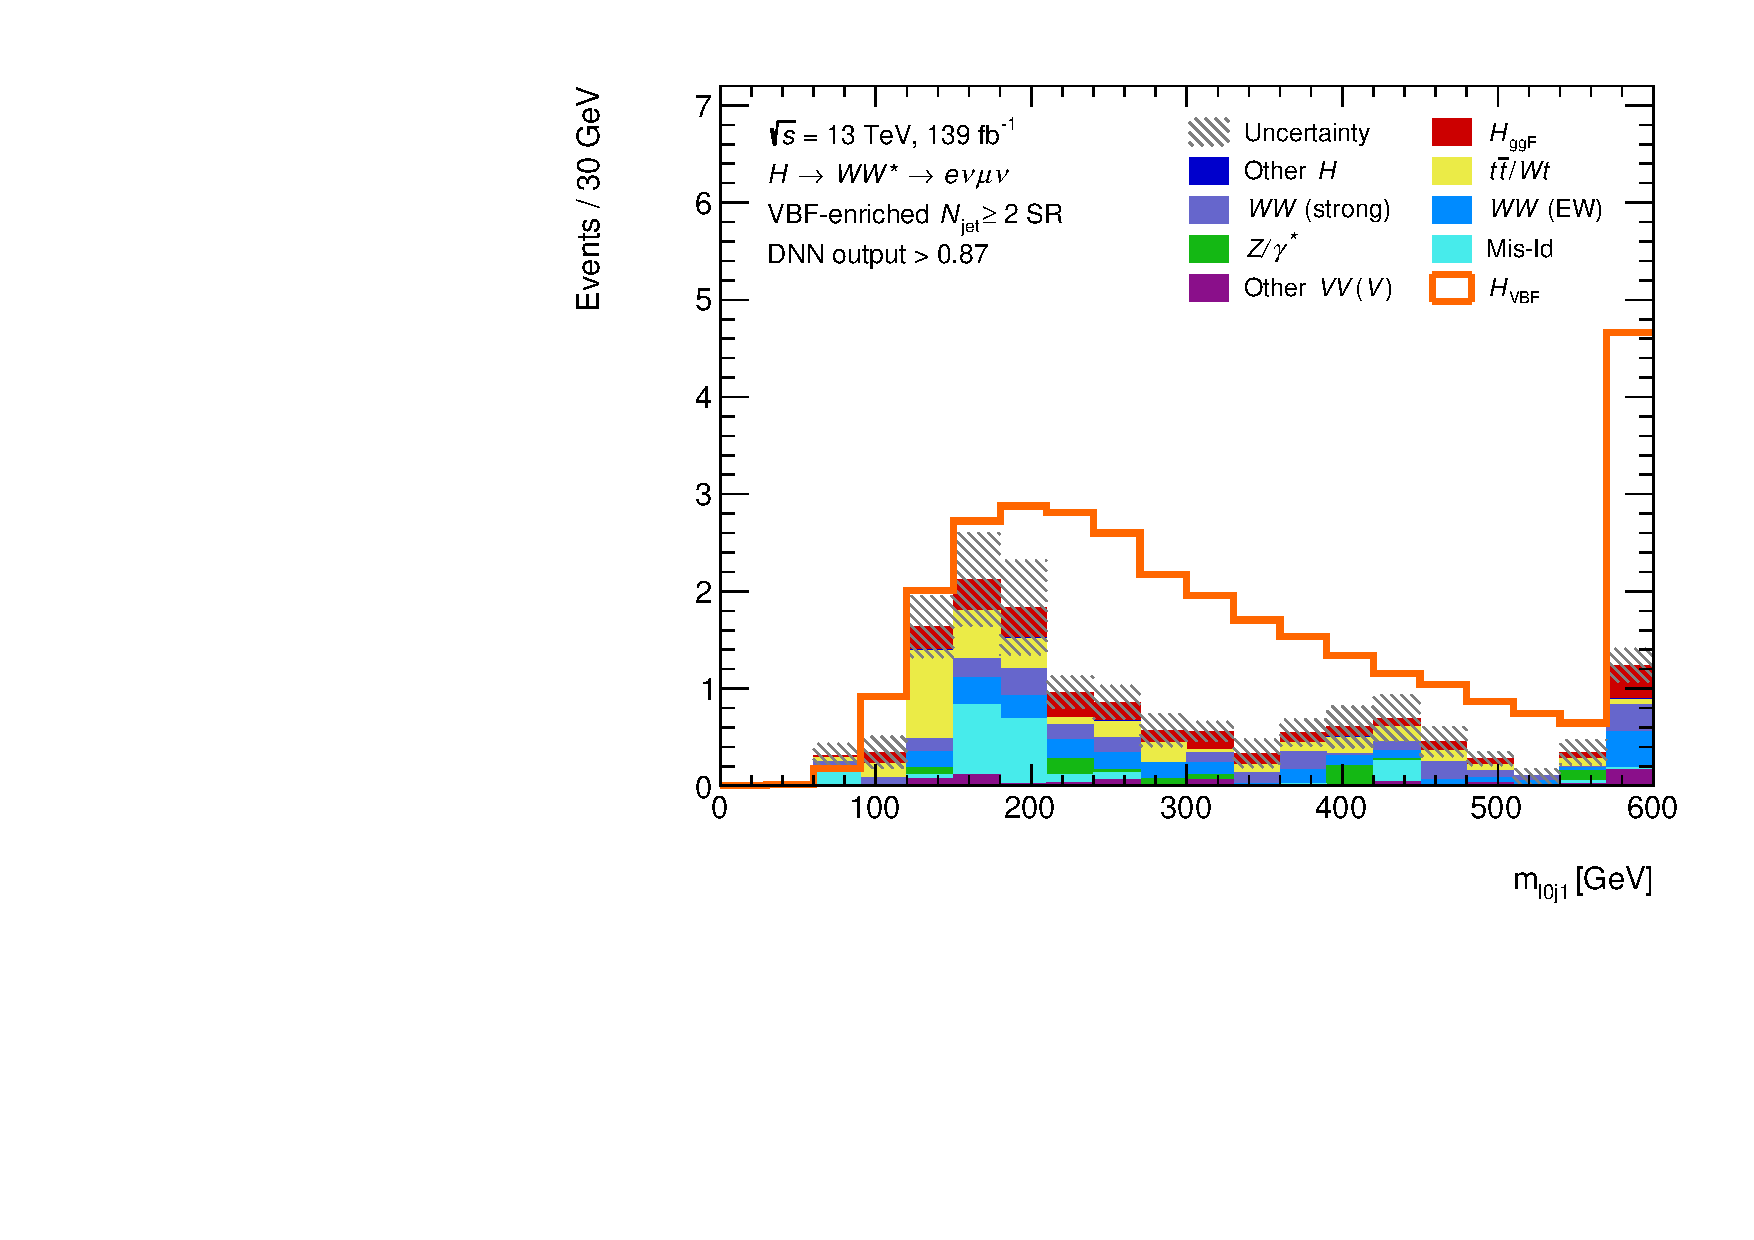
\includegraphics[width=0.32\textwidth]{figures/hww/dnn/blinded/run2-emme-CutVBFSR_DNN87-Ml0j1-lin.pdf}
    } \\
    \subfloat[$\mltwojtwo$]{
        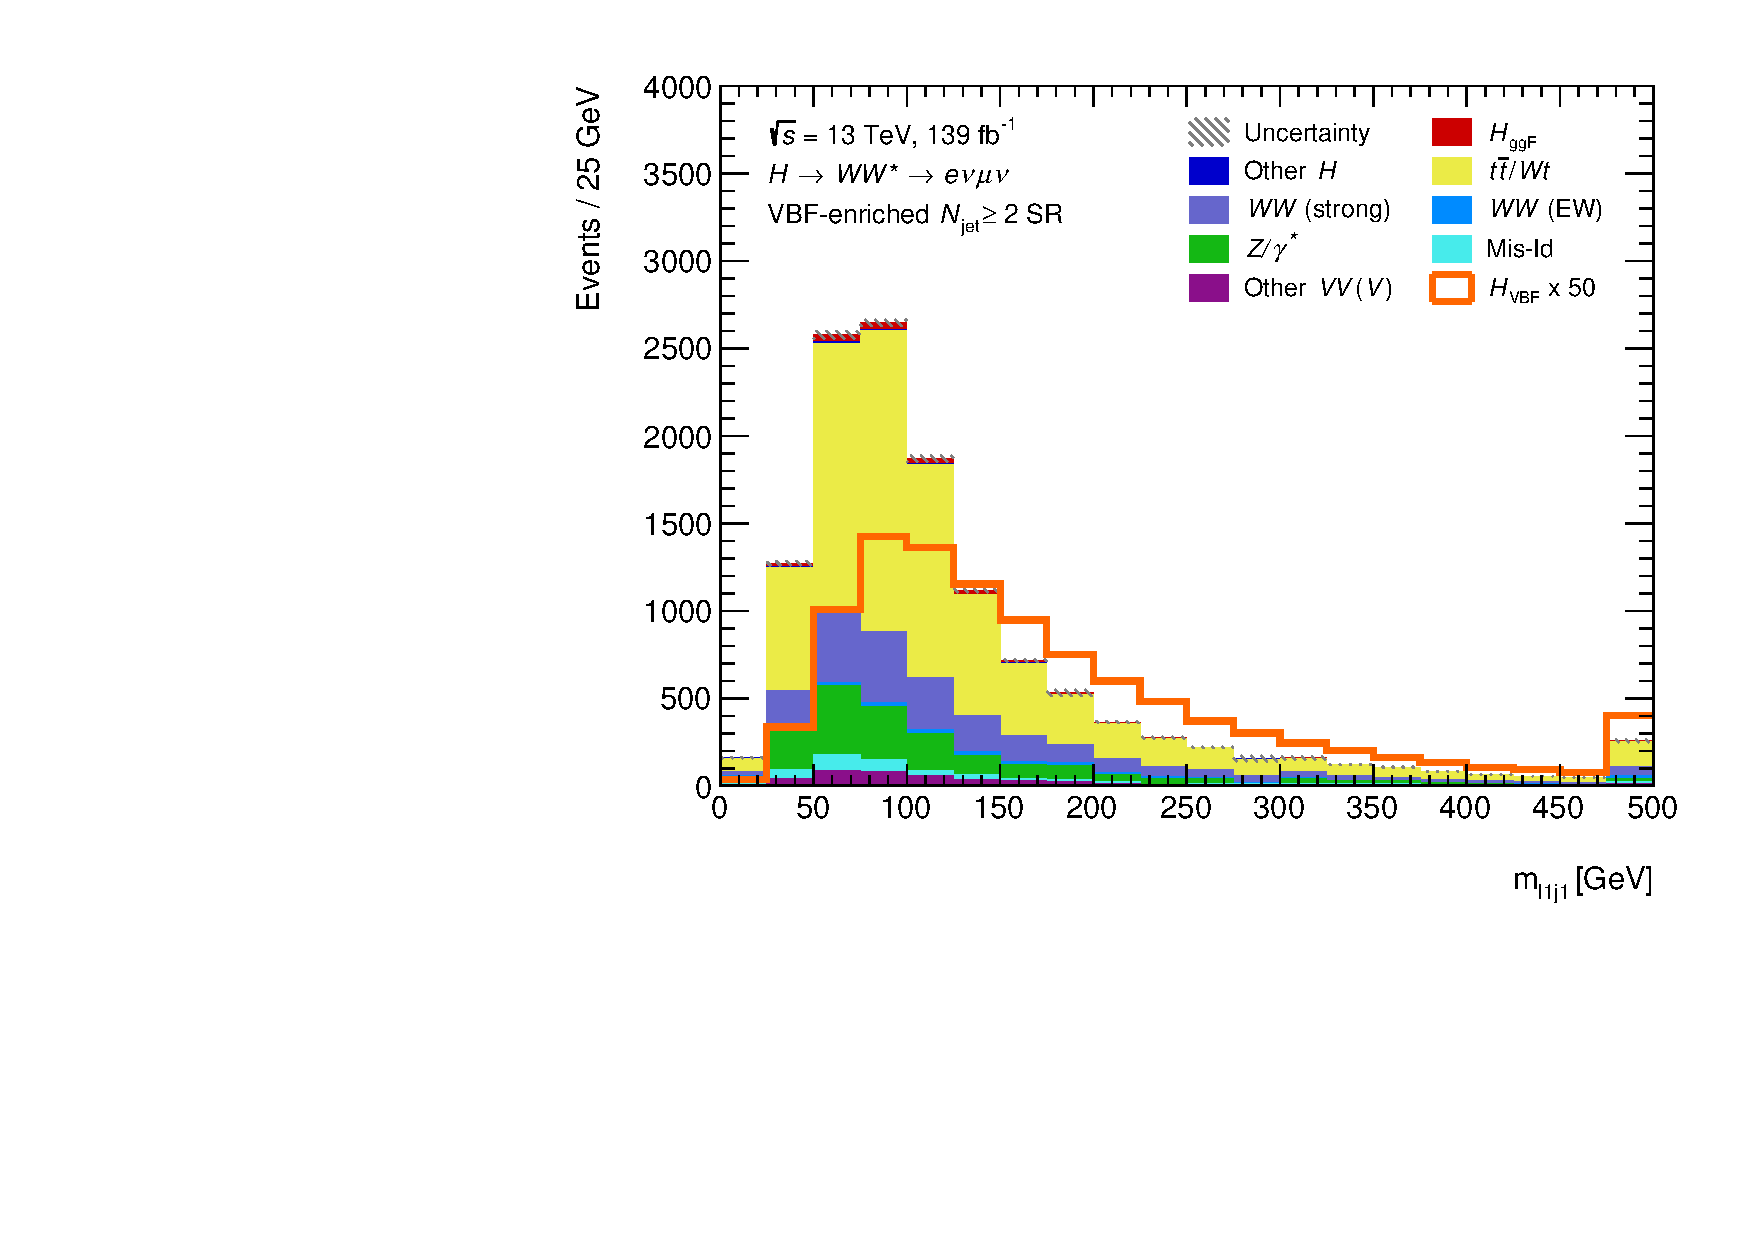
\includegraphics[width=0.32\textwidth]{figures/hww/dnn/blinded/run2-emme-CutVBF_SR-Ml1j1-lin.pdf} \hfill
        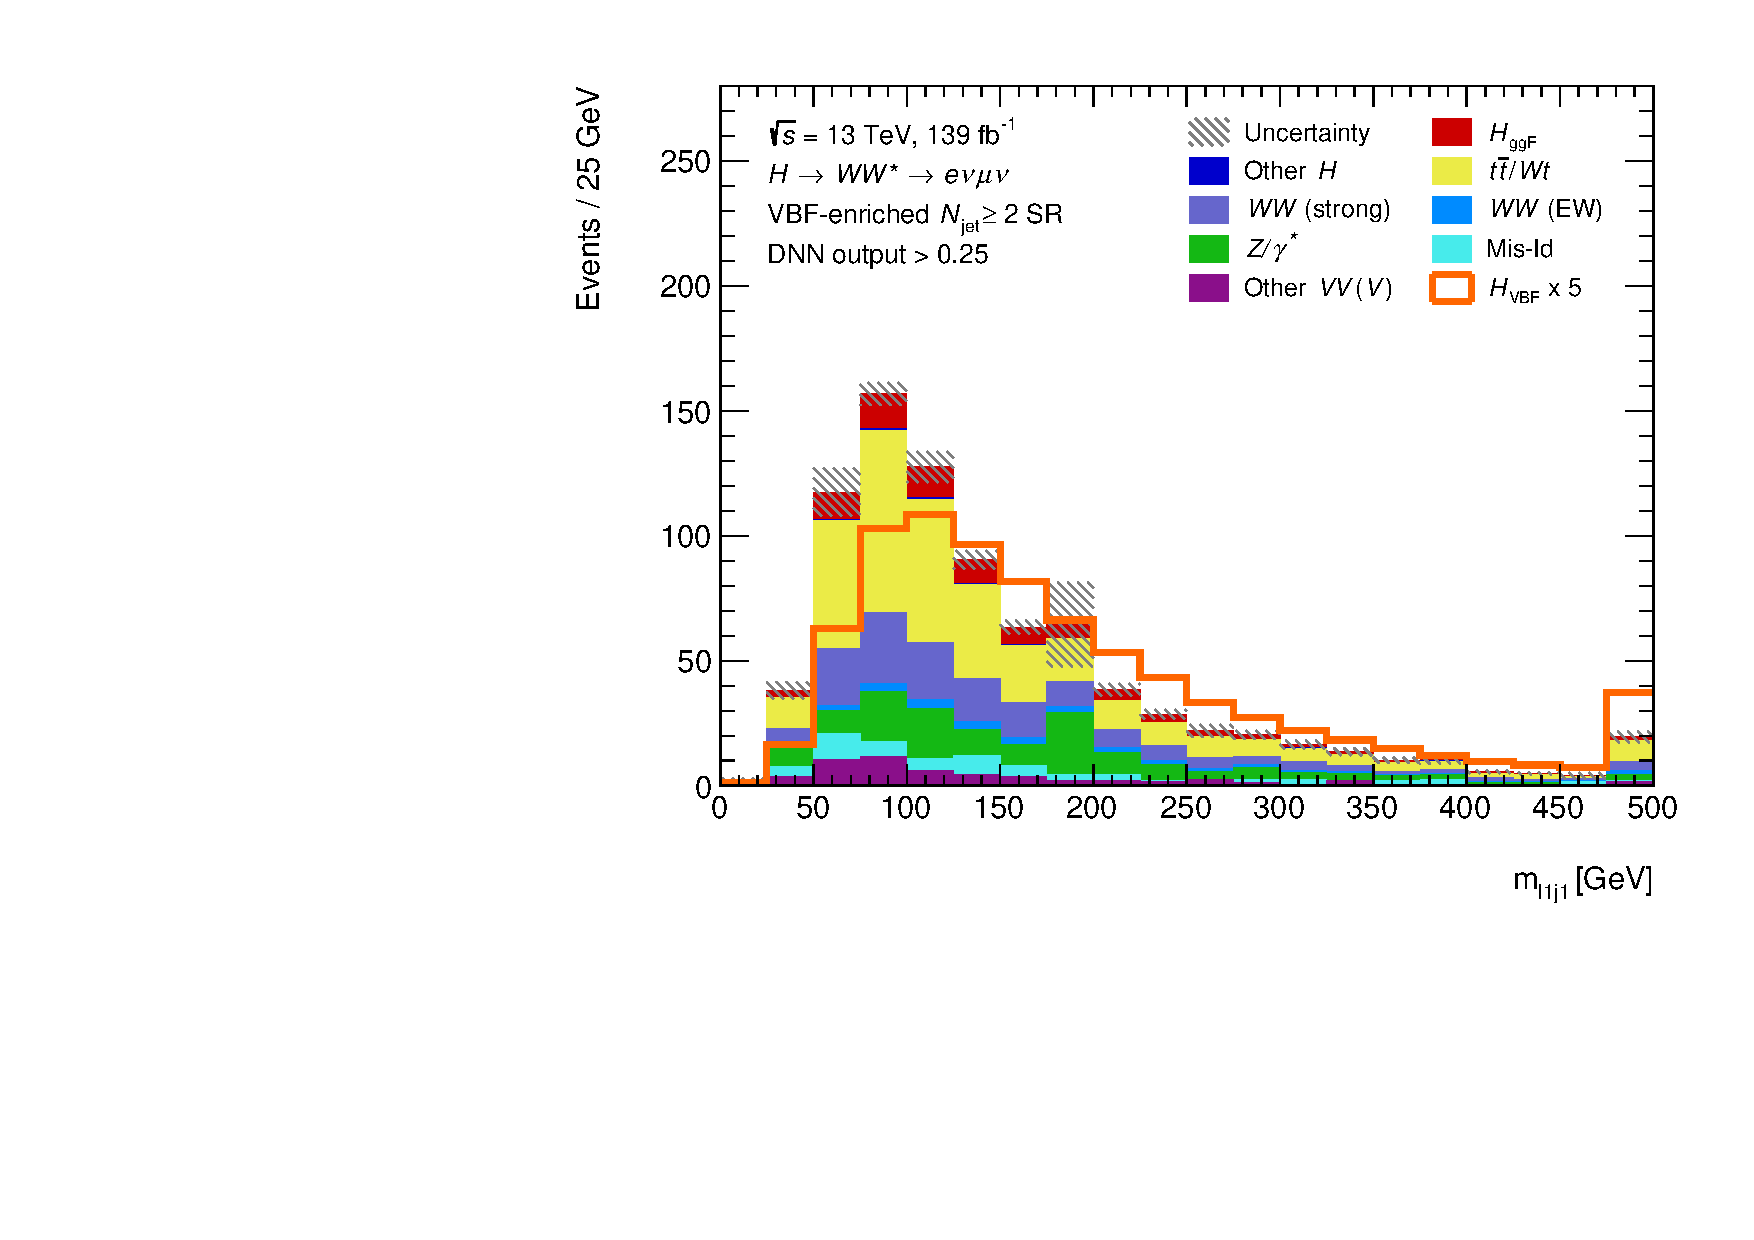
\includegraphics[width=0.32\textwidth]{figures/hww/dnn/blinded/run2-emme-CutVBFSR_DNN25-Ml1j1-lin.pdf} \hfill
        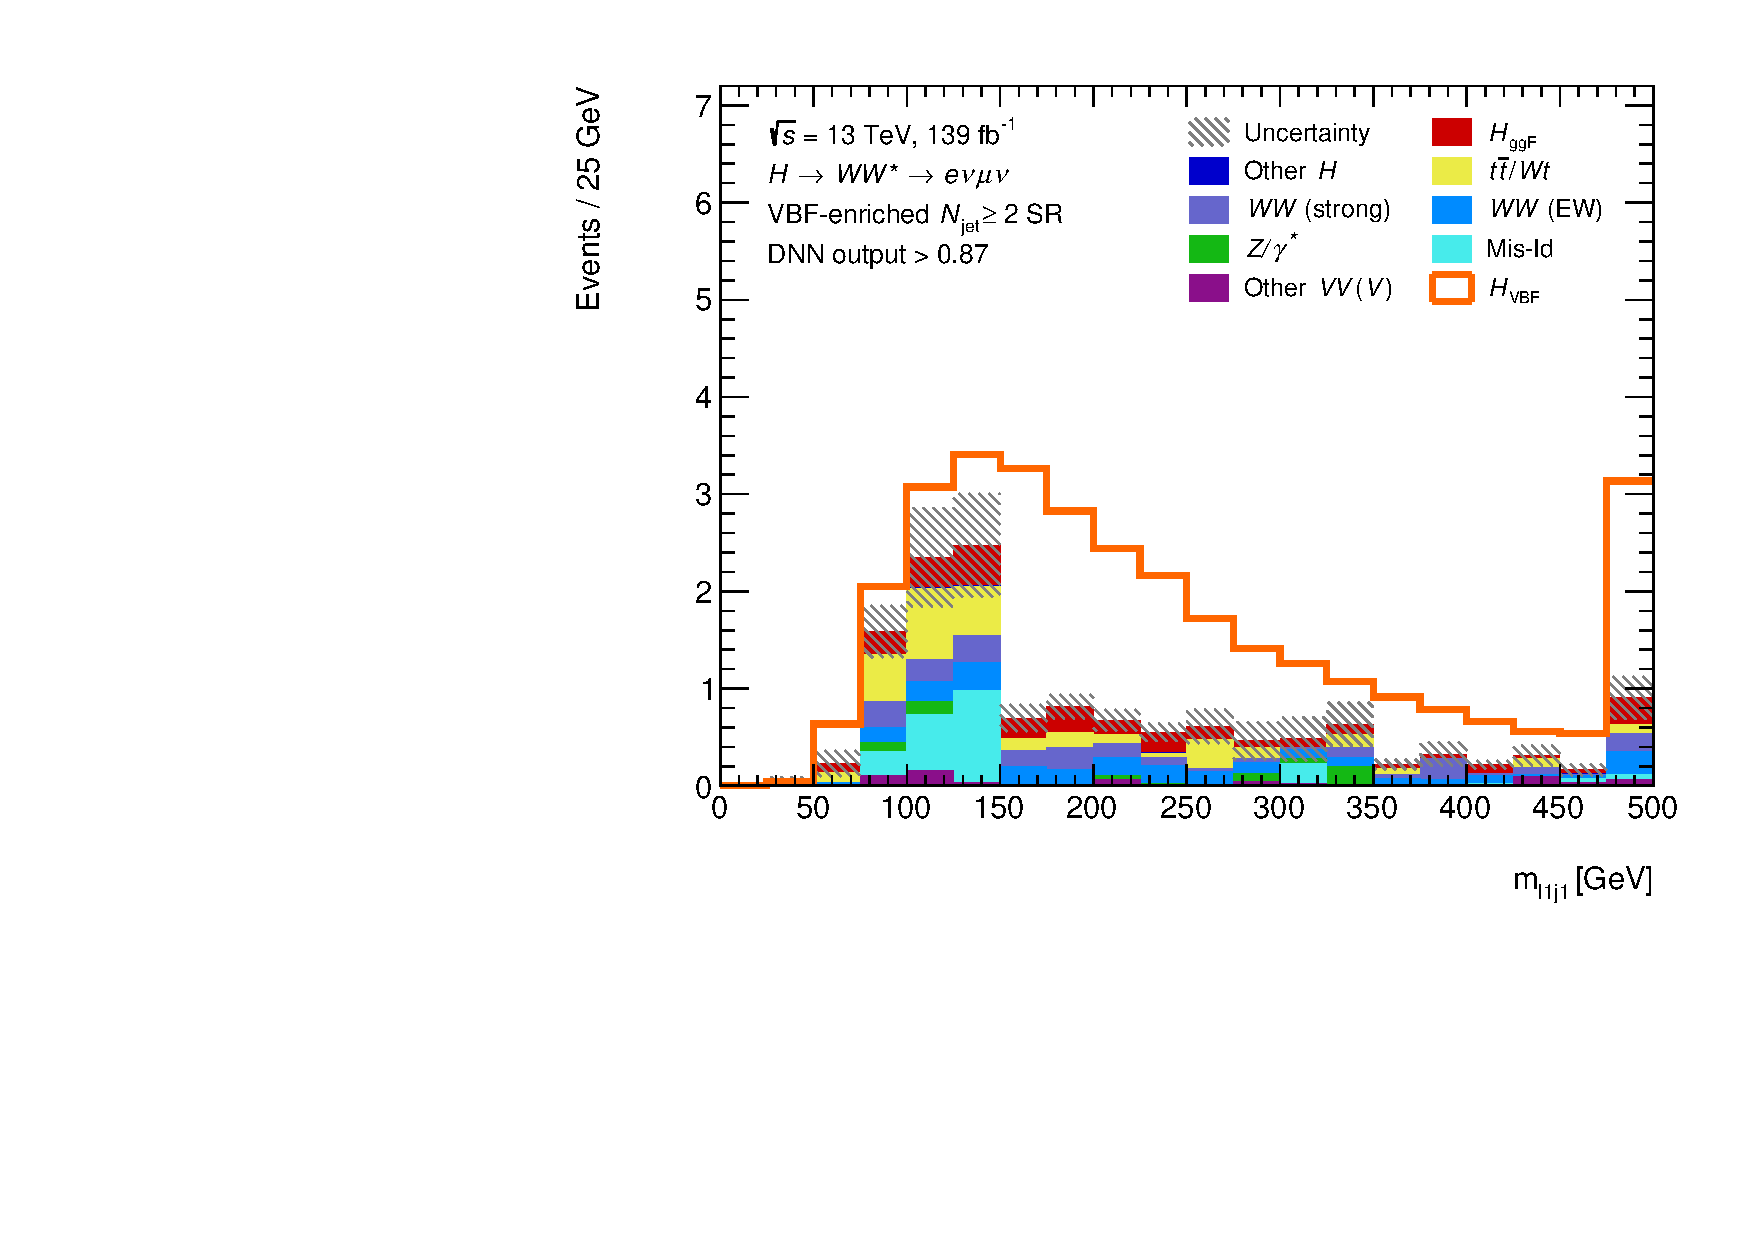
\includegraphics[width=0.32\textwidth]{figures/hww/dnn/blinded/run2-emme-CutVBFSR_DNN87-Ml1j1-lin.pdf}
    } 
    {\caption{Distributions of $\mlonejone$, $\mltwojone$, $\mlonejtwo$, and $\mltwojtwo$ in the VBF signal region.
            Each row shows one variable with different cuts on the DNN output distribution being applied in different columns.
            \label{fig:vbf:blindedSR3} }}
\end{figure}

\captionsetup[subfloat]{captionskip=3pt} % space between subfloat caption and image